% Automatically generated figure inventory for task6.

\begin{figure}[H]
\centering
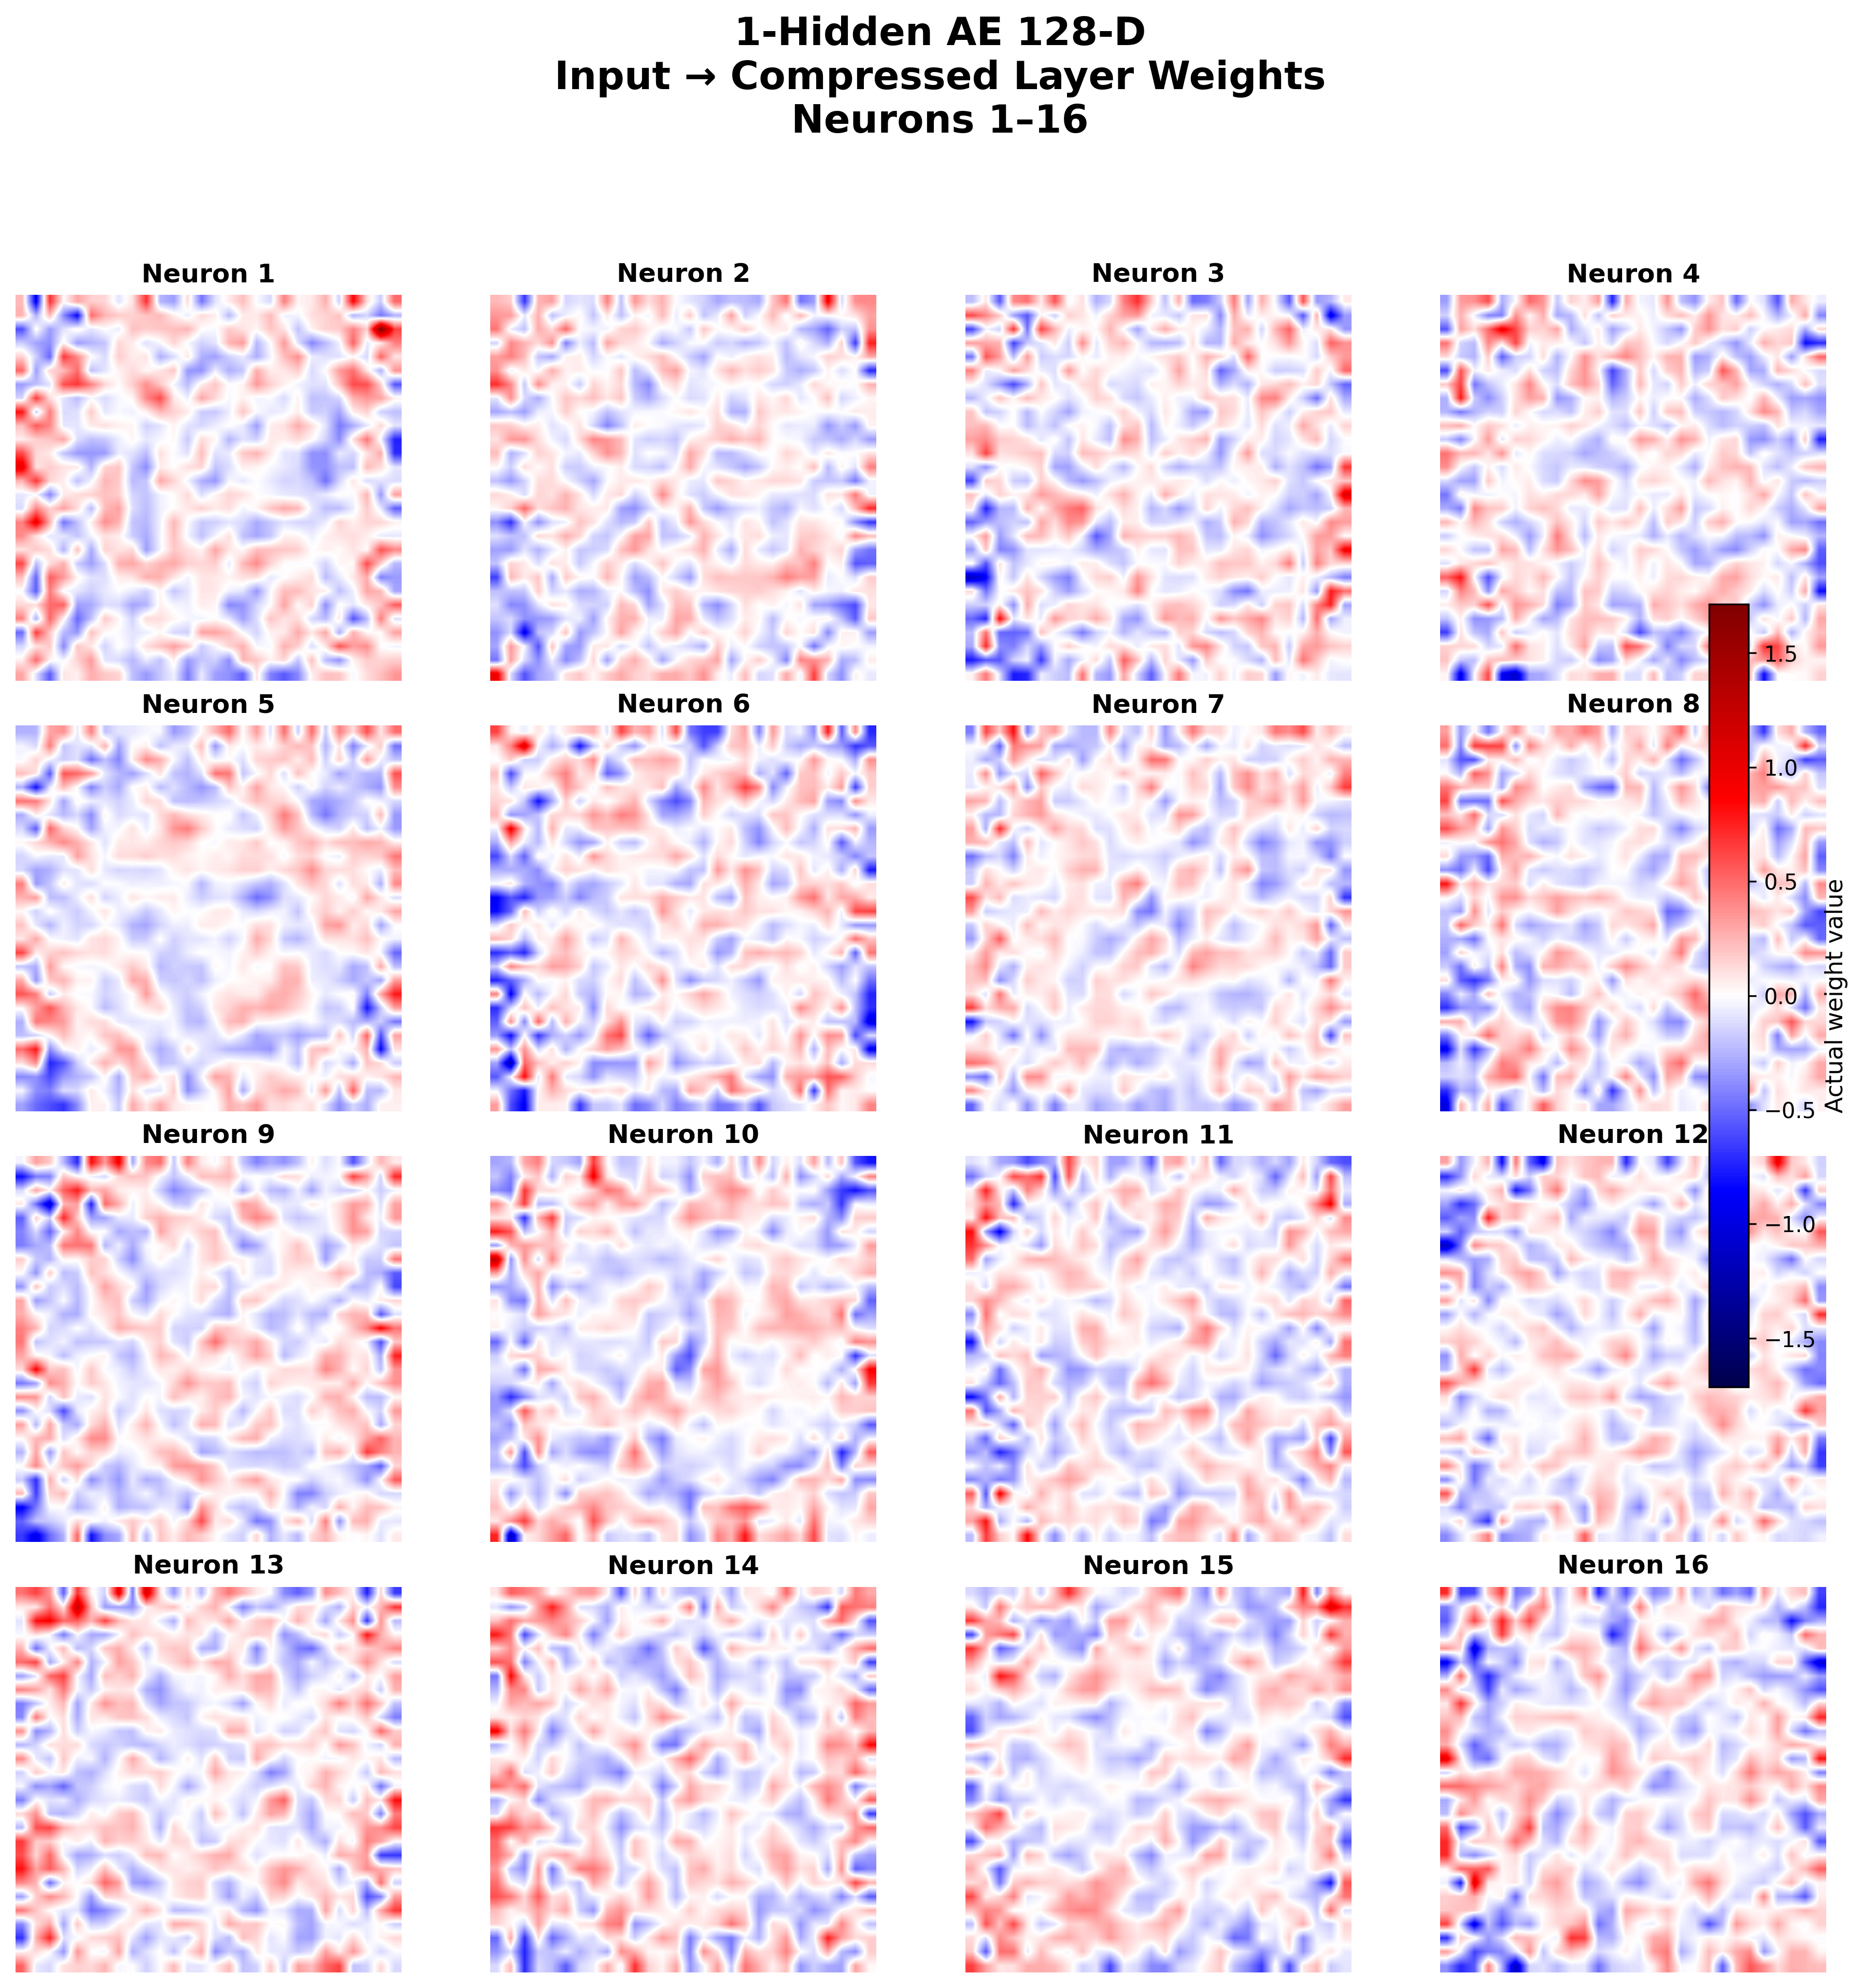
\includegraphics[width=0.99\linewidth,height=0.72\textheight,keepaspectratio]{figures/task6/1_hidden_ae/neurons_001_016.png}
\caption{Input-to-bottleneck weight visualization for neurons 1--16.}
\label{fig:task6_1}
\end{figure}

\begin{figure}[H]
\centering
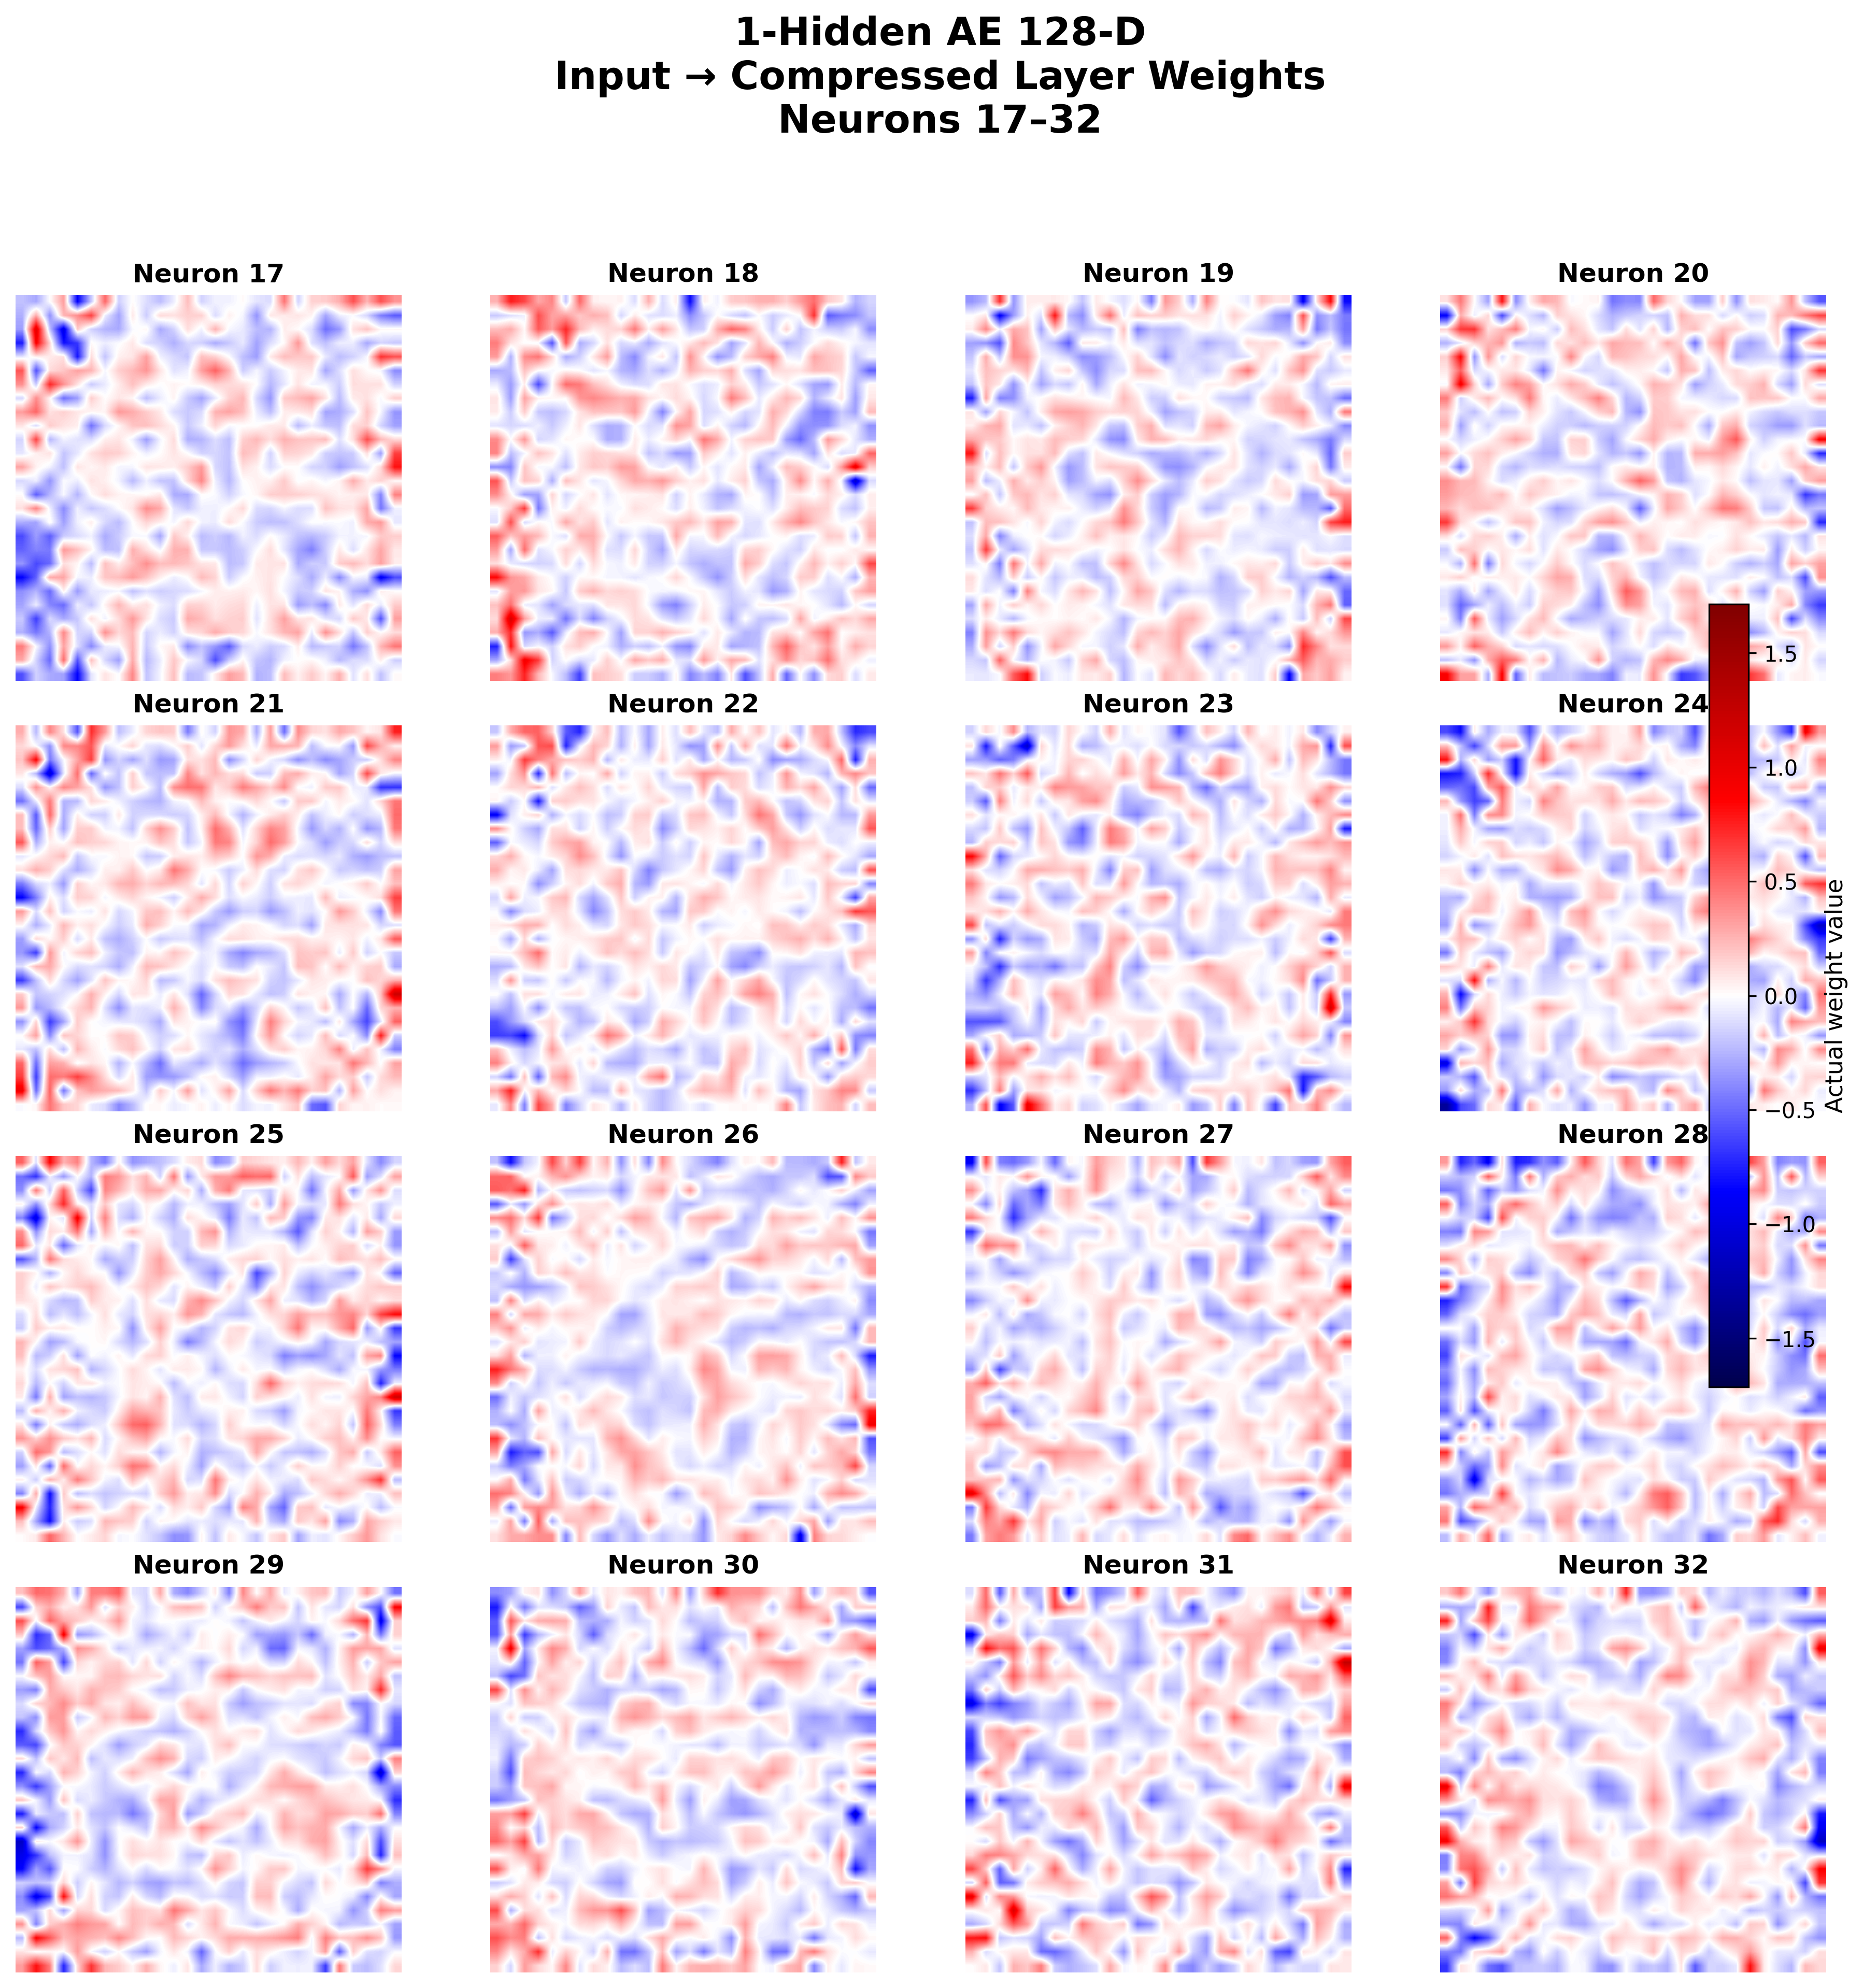
\includegraphics[width=0.99\linewidth,height=0.72\textheight,keepaspectratio]{figures/task6/1_hidden_ae/neurons_017_032.png}
\caption{Input-to-bottleneck weight visualization for neurons 17--32.}
\label{fig:task6_2}
\end{figure}

\begin{figure}[H]
\centering
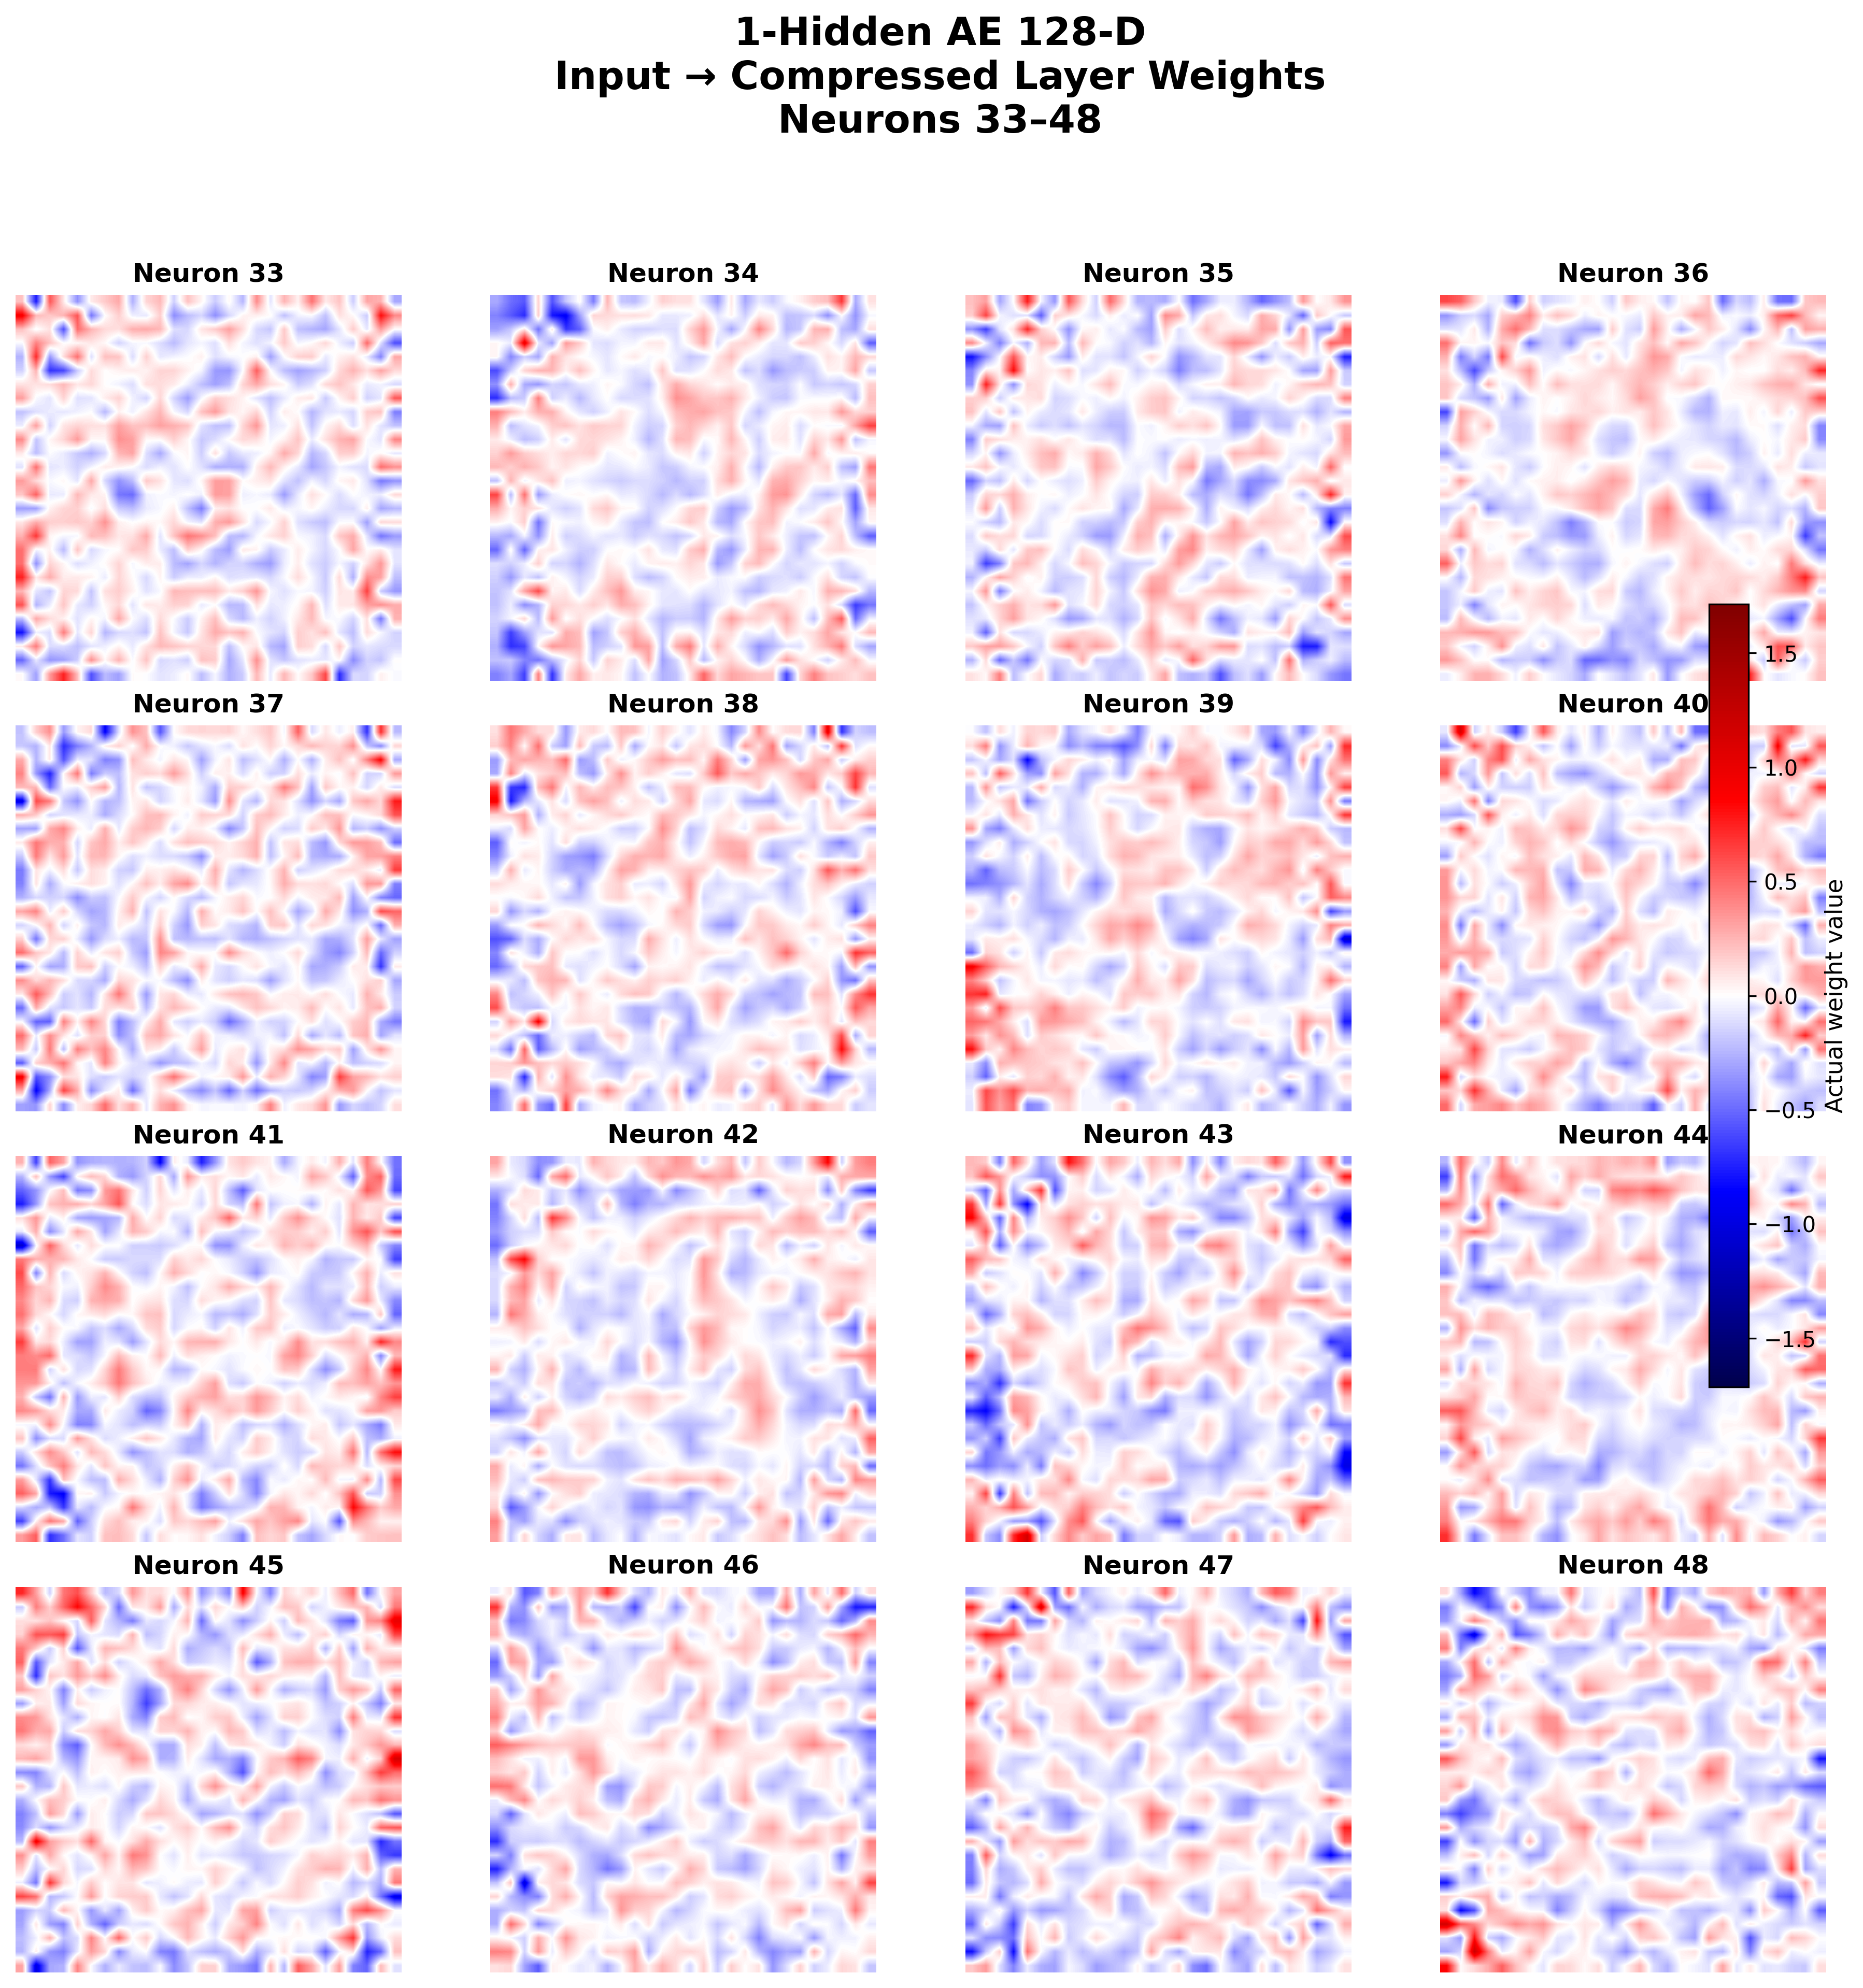
\includegraphics[width=0.99\linewidth,height=0.72\textheight,keepaspectratio]{figures/task6/1_hidden_ae/neurons_033_048.png}
\caption{Input-to-bottleneck weight visualization for neurons 33--48.}
\label{fig:task6_3}
\end{figure}

\begin{figure}[H]
\centering
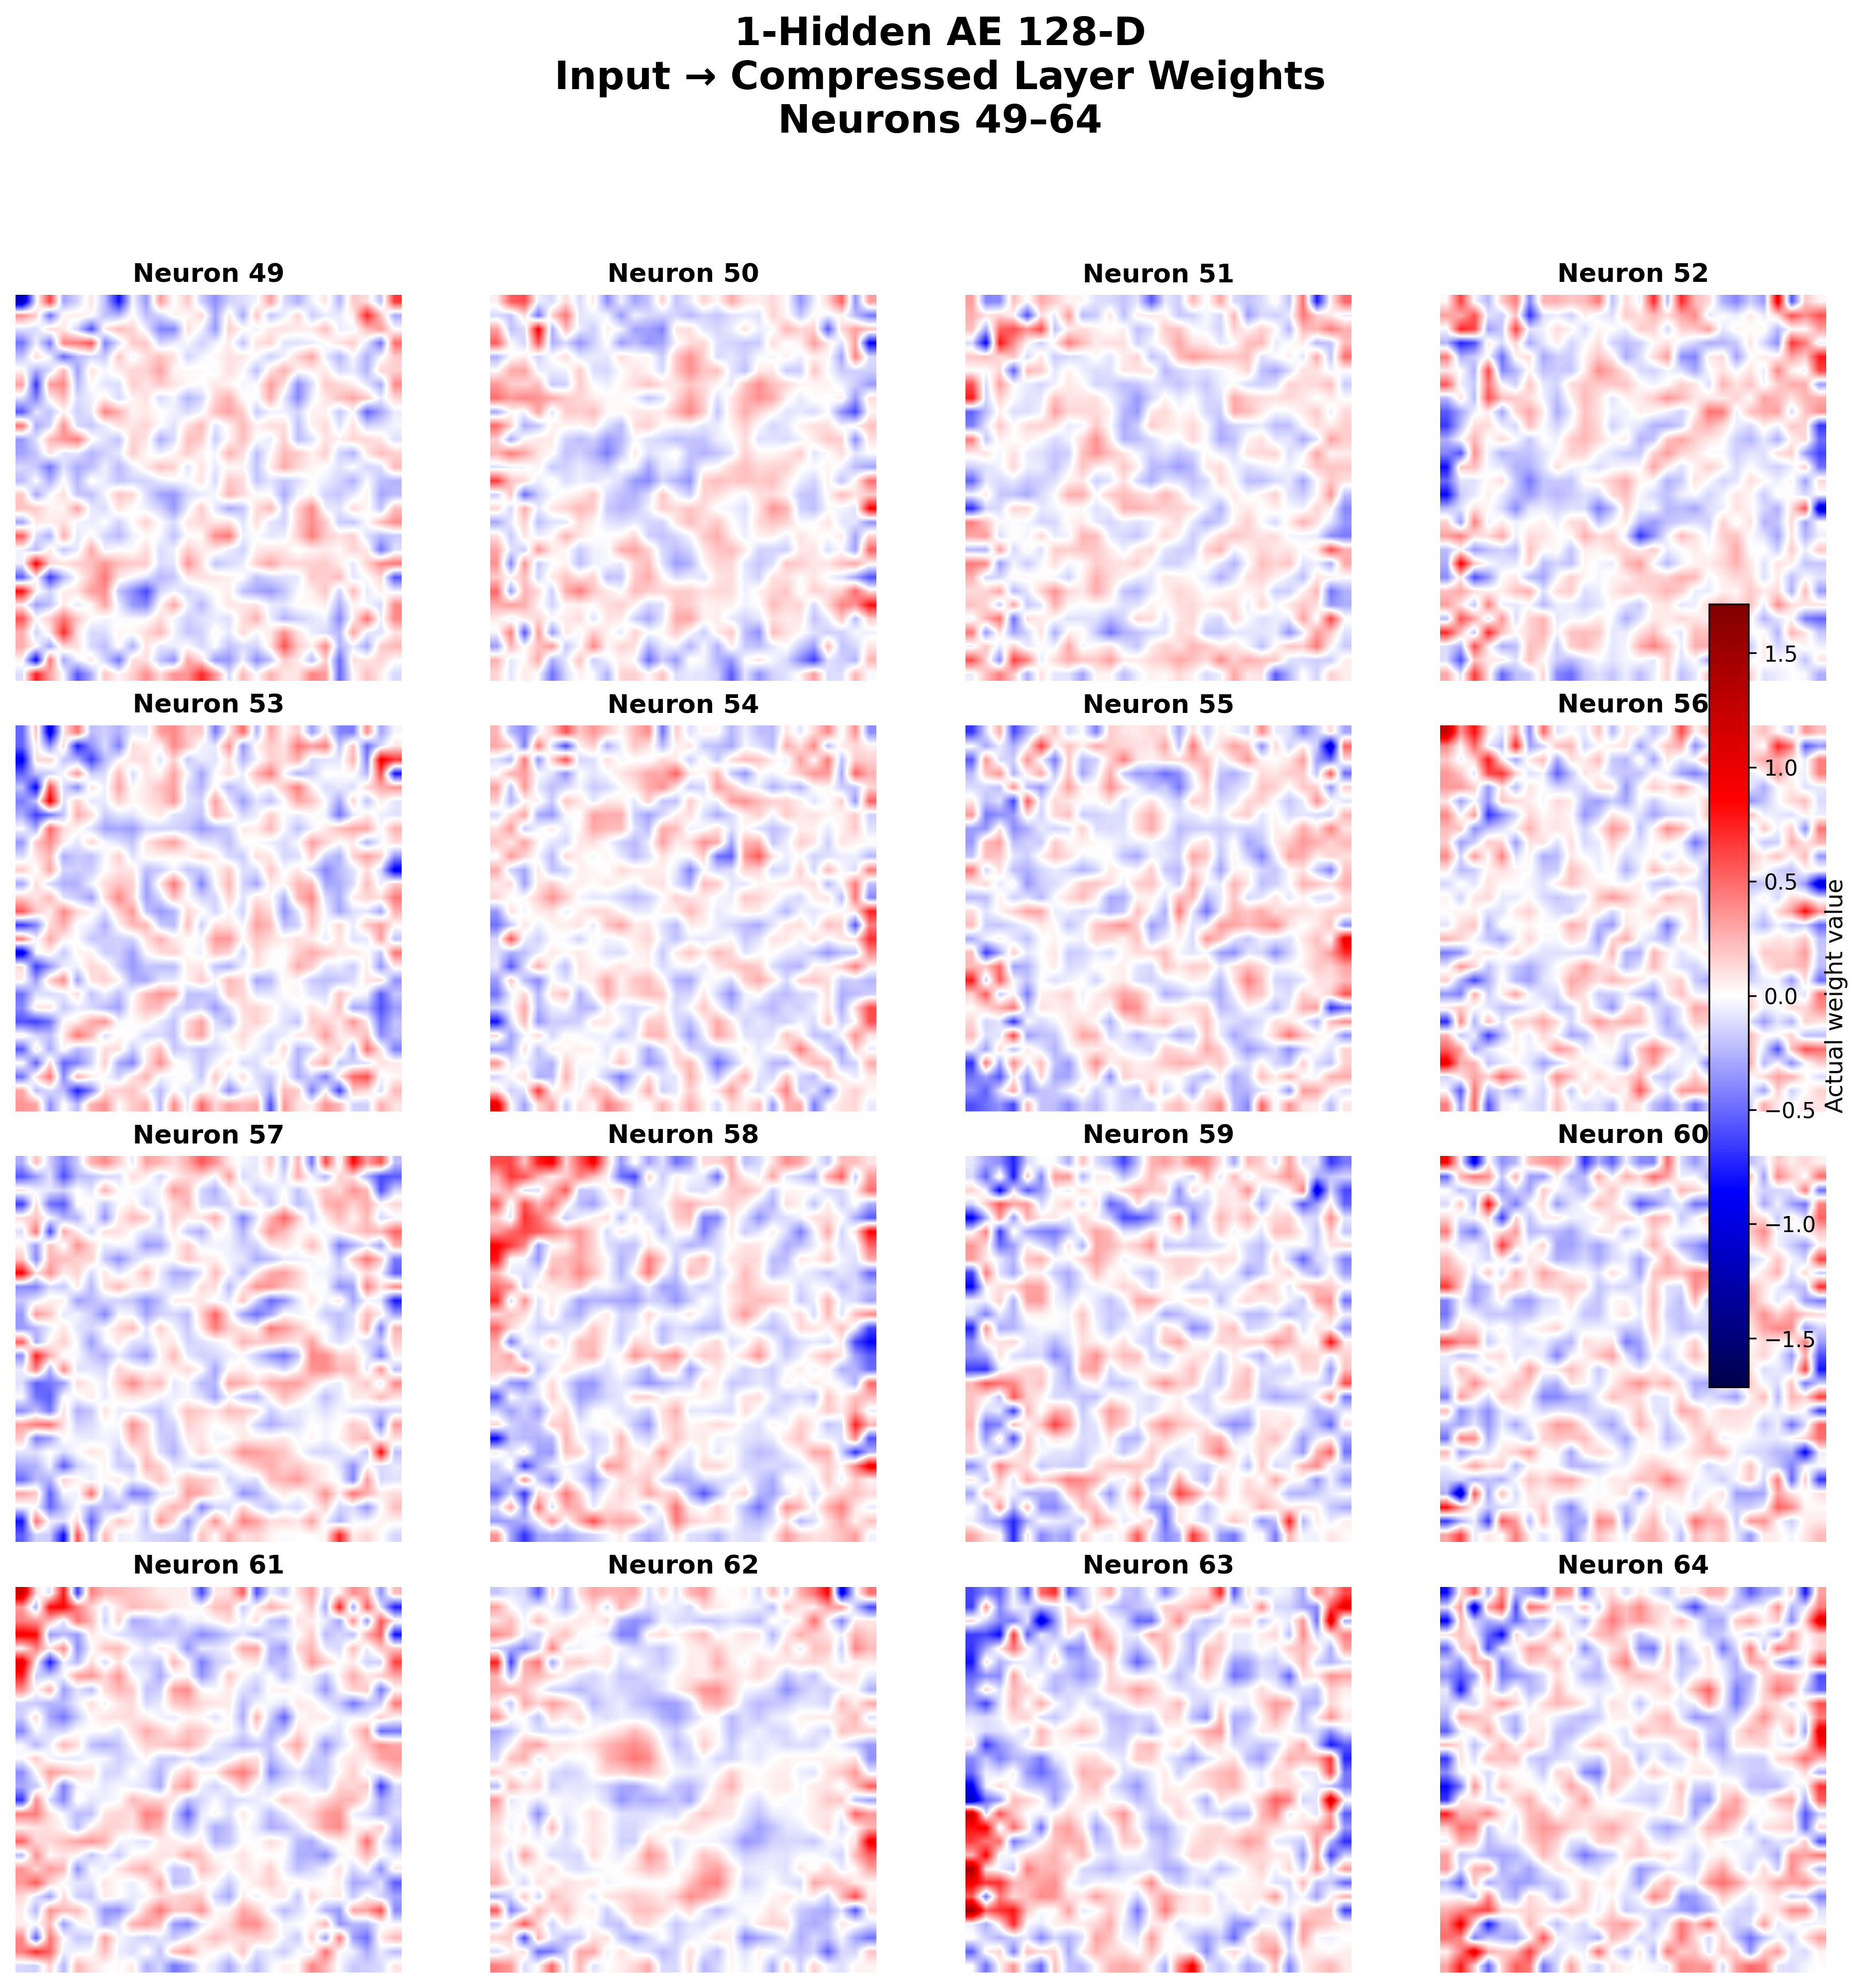
\includegraphics[width=0.99\linewidth,height=0.72\textheight,keepaspectratio]{figures/task6/1_hidden_ae/neurons_049_064.png}
\caption{Input-to-bottleneck weight visualization for neurons 49--64.}
\label{fig:task6_4}
\end{figure}

\begin{figure}[H]
\centering
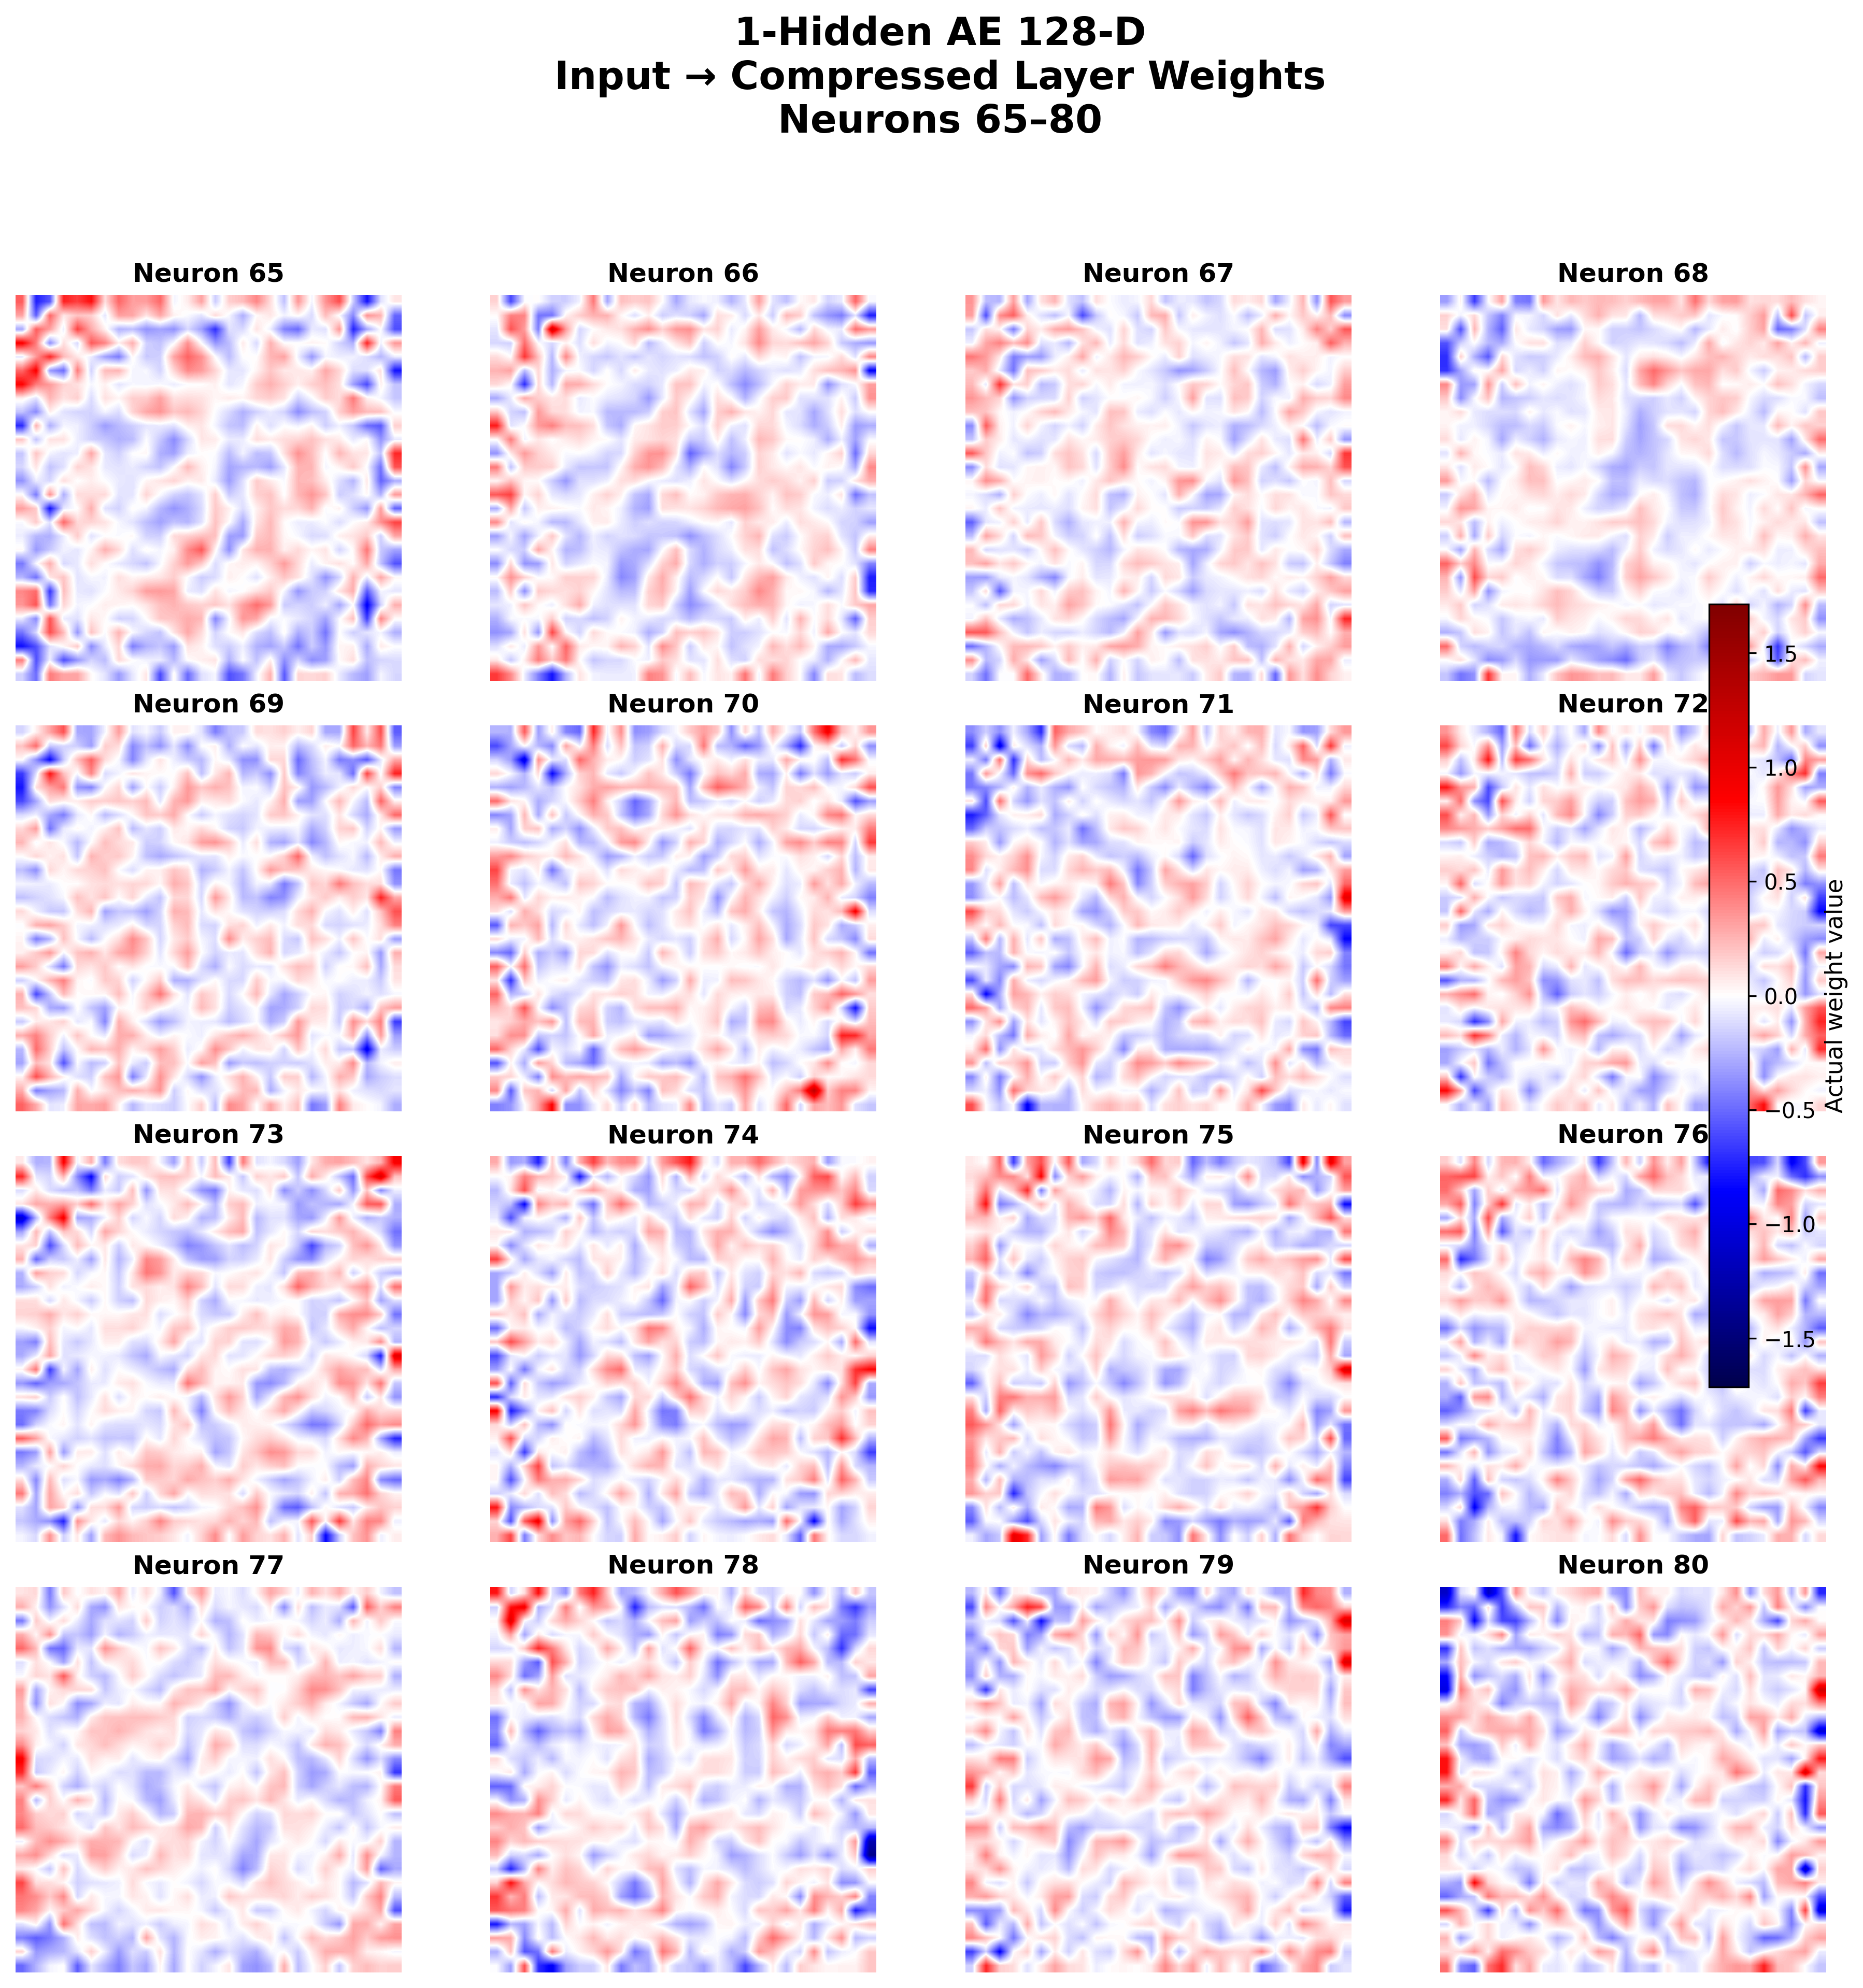
\includegraphics[width=0.99\linewidth,height=0.72\textheight,keepaspectratio]{figures/task6/1_hidden_ae/neurons_065_080.png}
\caption{Input-to-bottleneck weight visualization for neurons 65--80.}
\label{fig:task6_5}
\end{figure}

\begin{figure}[H]
\centering
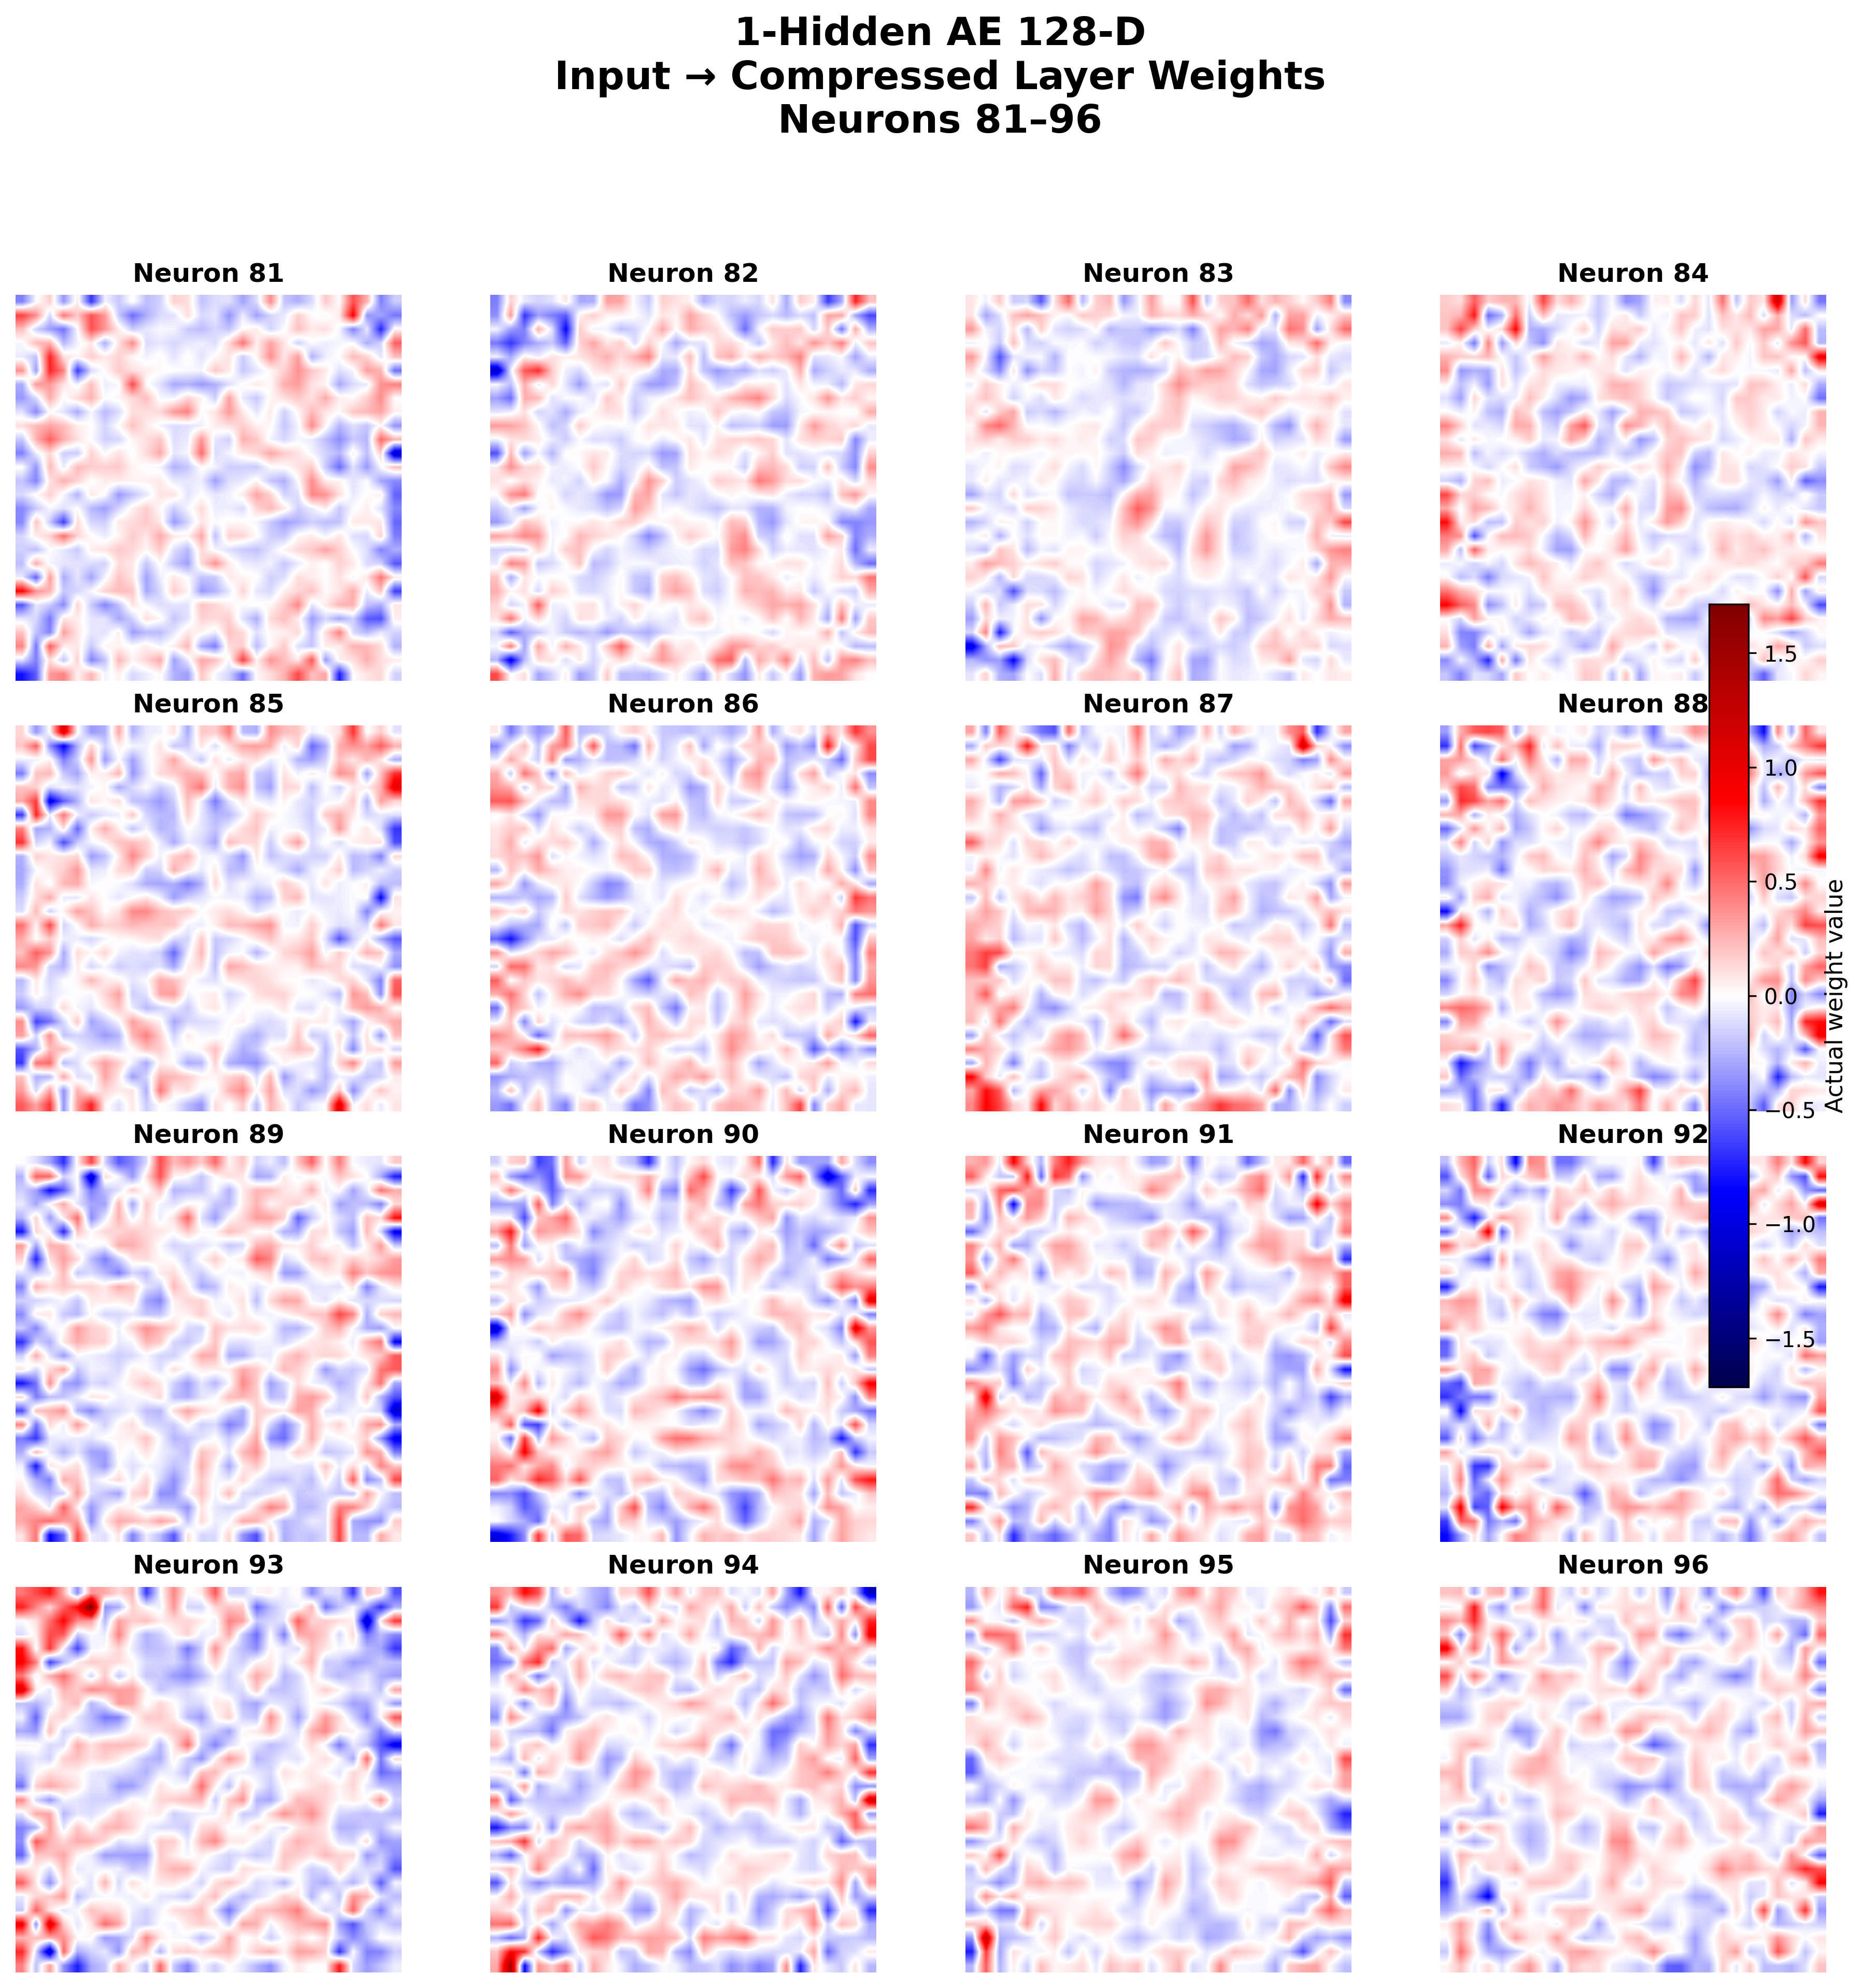
\includegraphics[width=0.99\linewidth,height=0.72\textheight,keepaspectratio]{figures/task6/1_hidden_ae/neurons_081_096.png}
\caption{Input-to-bottleneck weight visualization for neurons 81--96.}
\label{fig:task6_6}
\end{figure}

\begin{figure}[H]
\centering
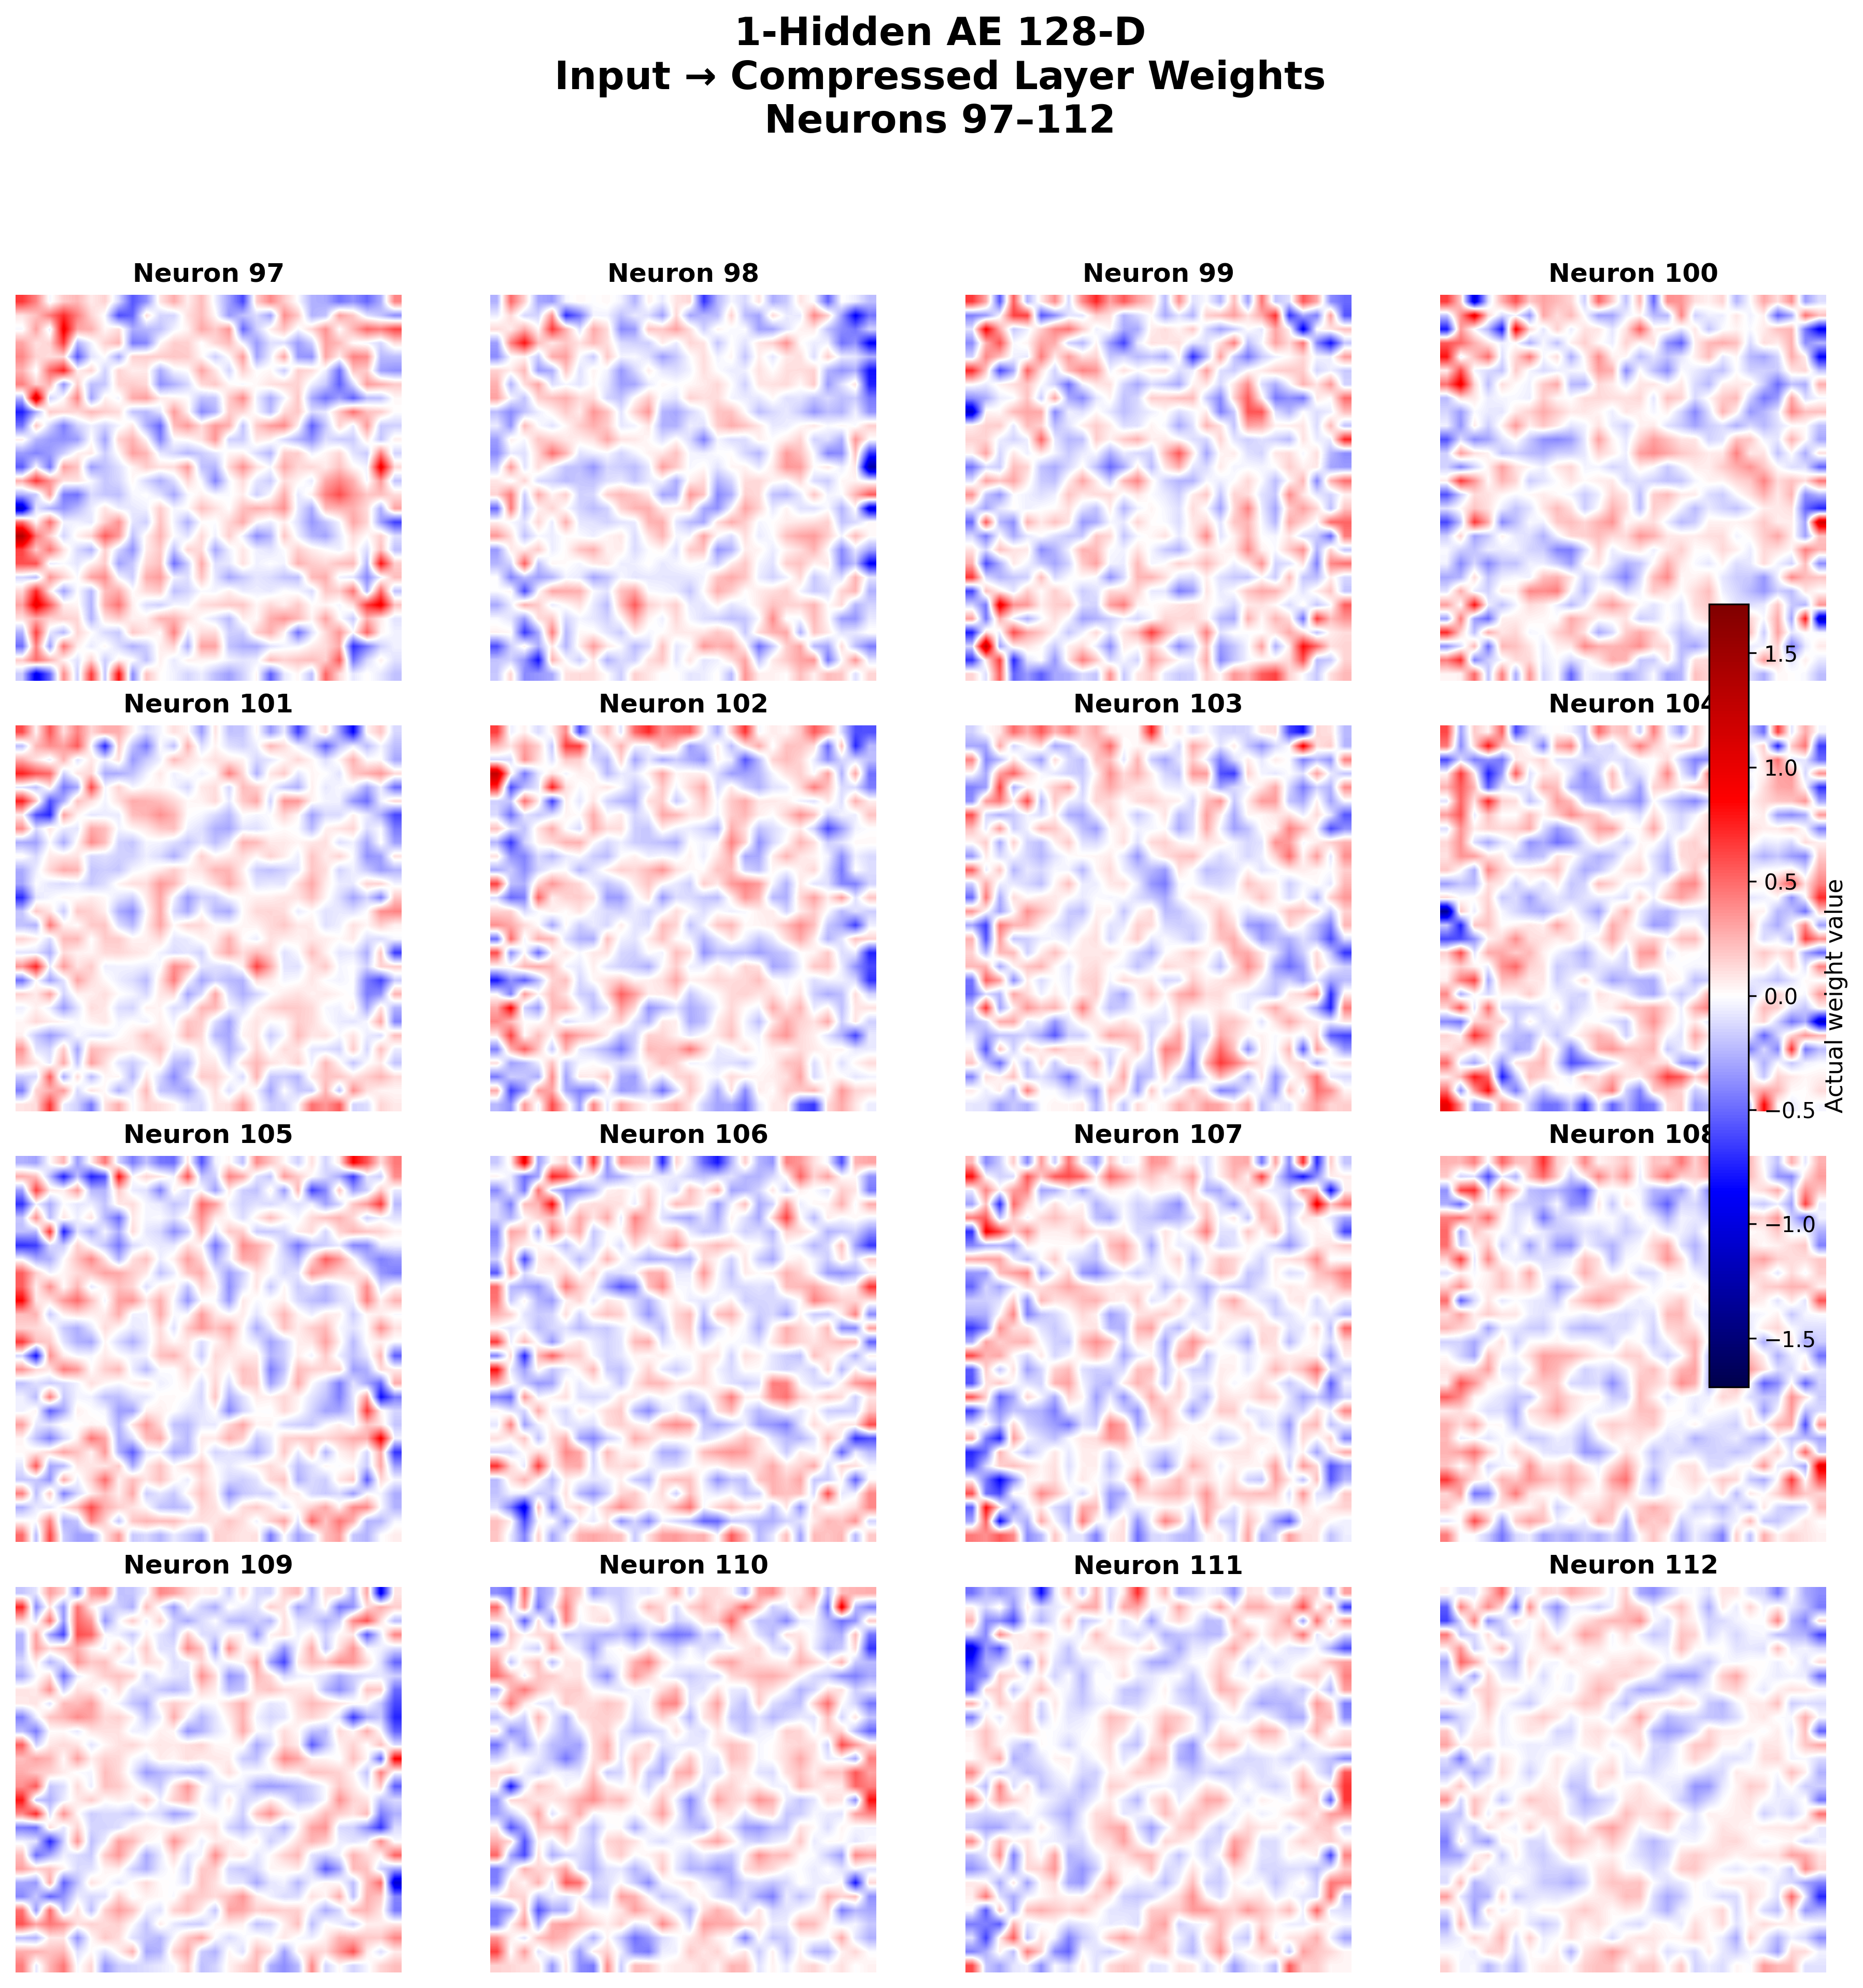
\includegraphics[width=0.99\linewidth,height=0.72\textheight,keepaspectratio]{figures/task6/1_hidden_ae/neurons_097_112.png}
\caption{Input-to-bottleneck weight visualization for neurons 97--112.}
\label{fig:task6_7}
\end{figure}

\begin{figure}[H]
\centering
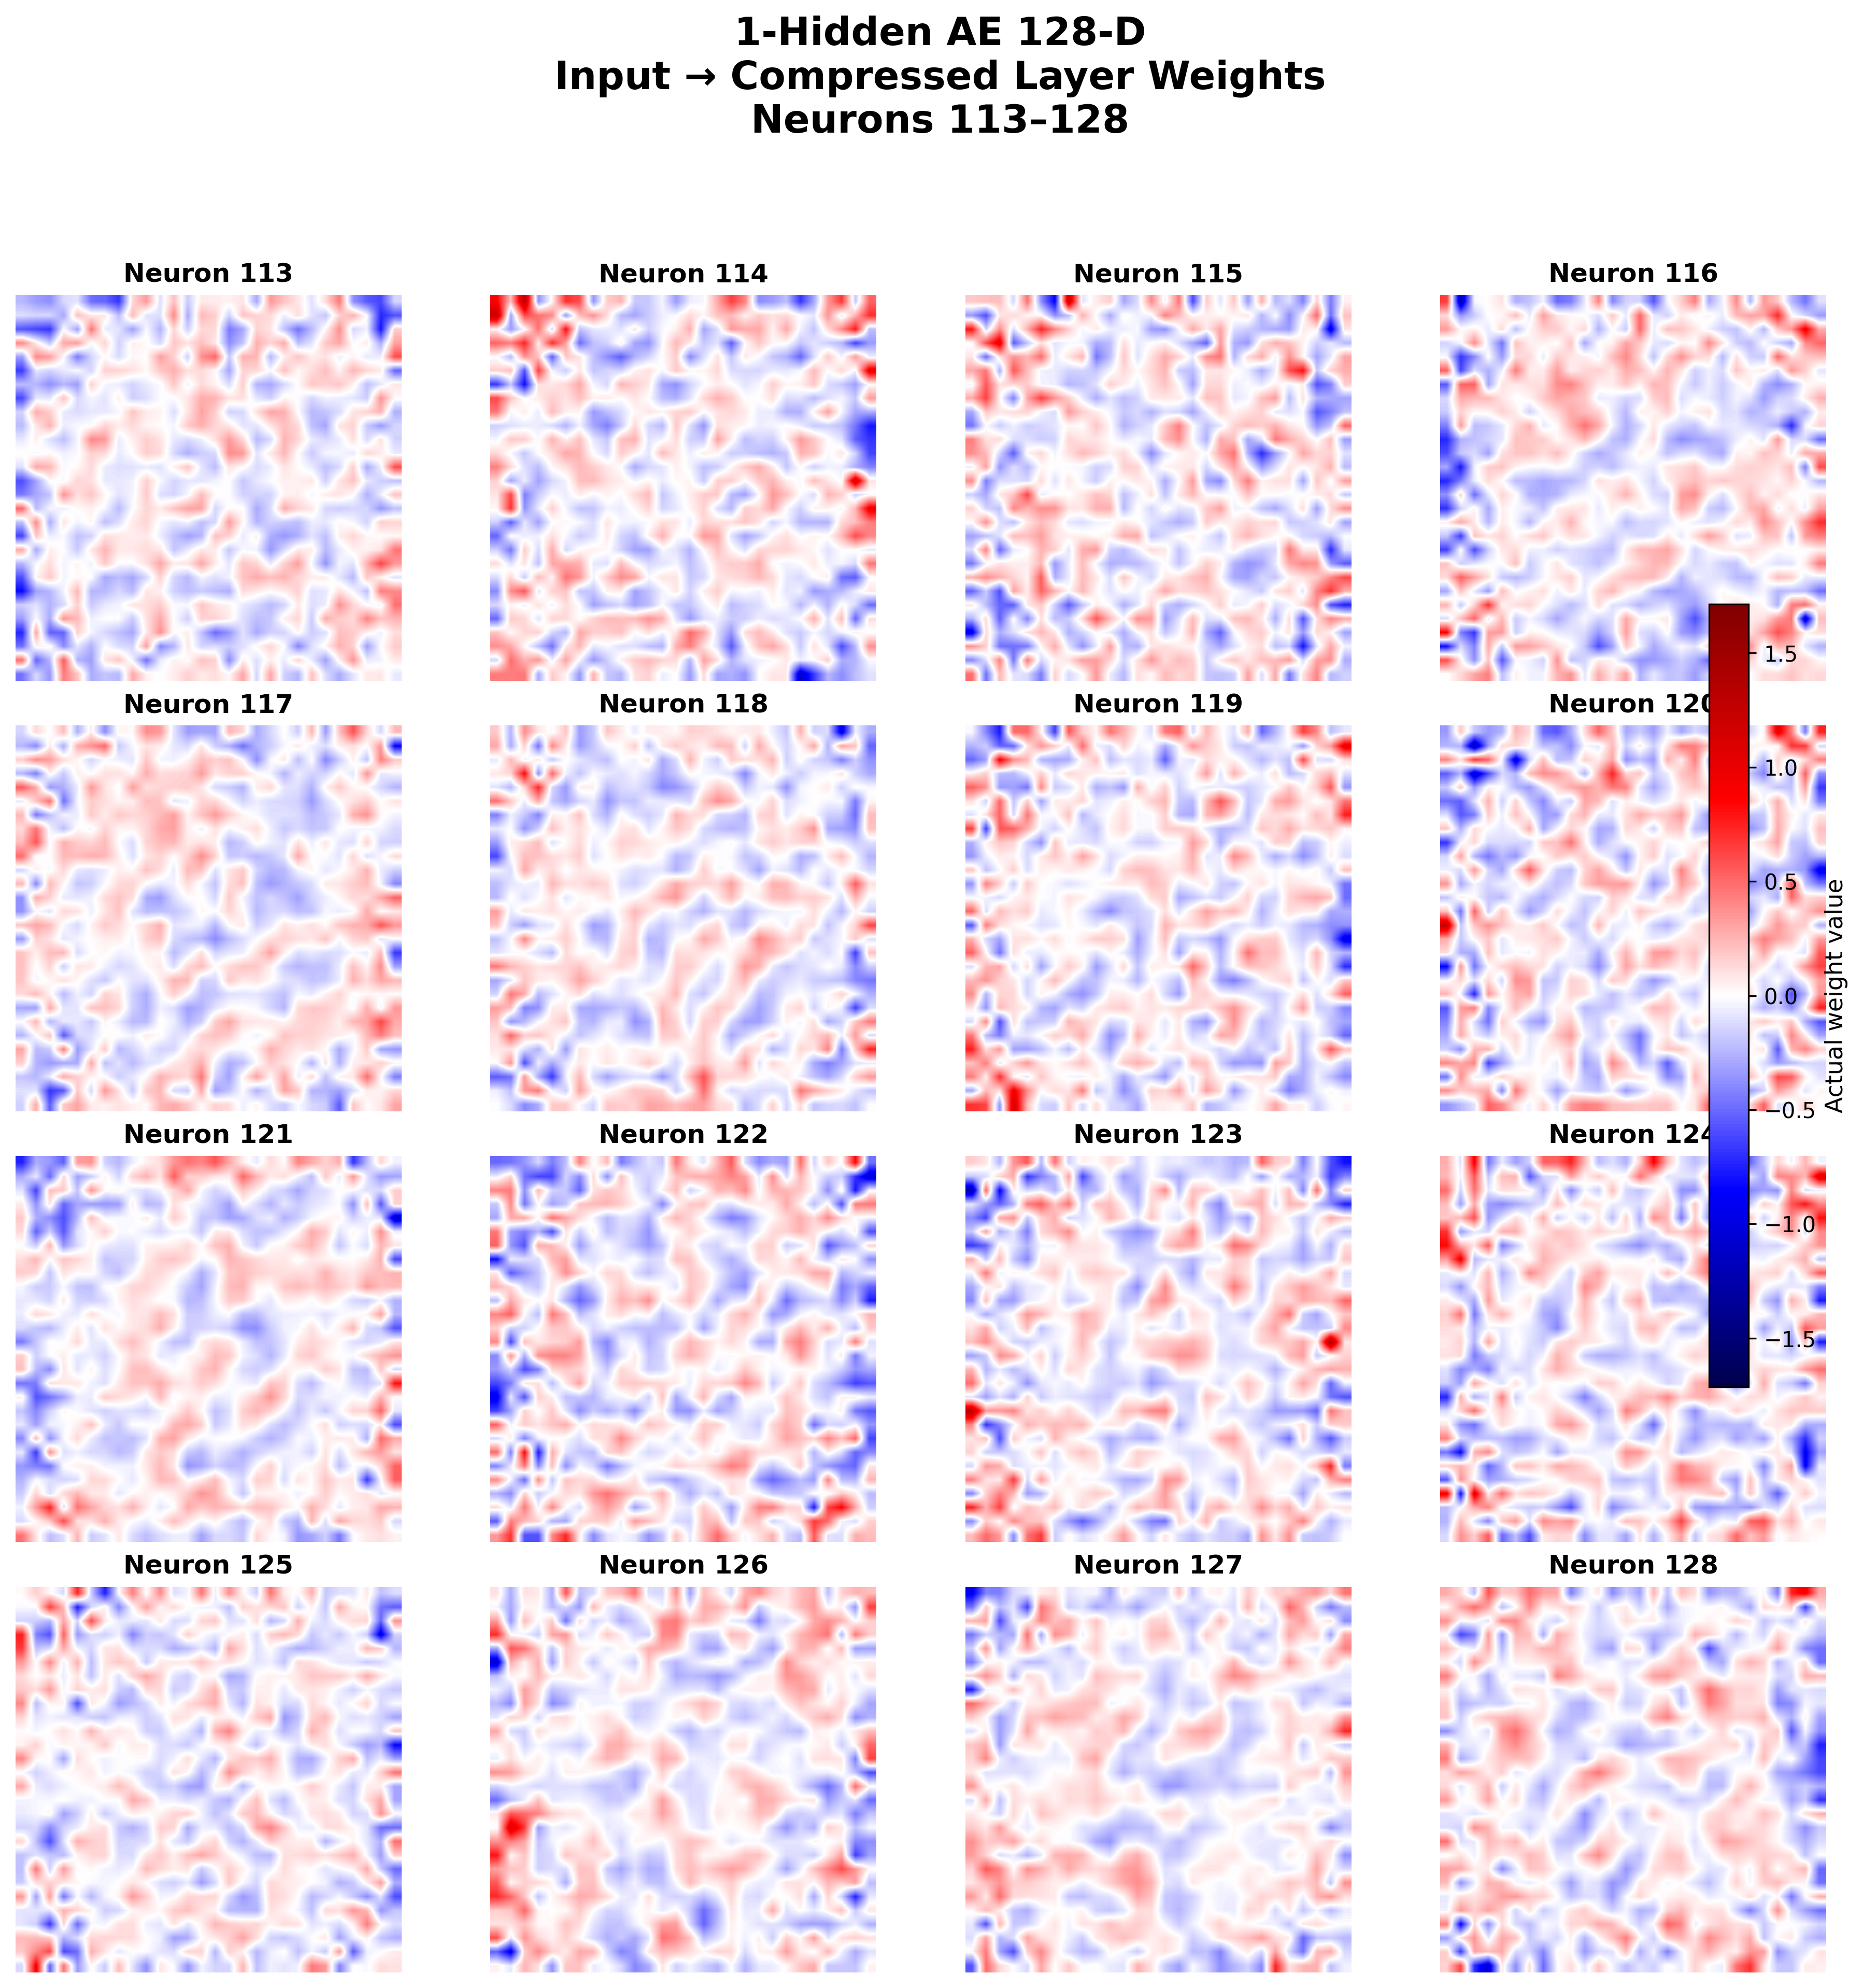
\includegraphics[width=0.99\linewidth,height=0.72\textheight,keepaspectratio]{figures/task6/1_hidden_ae/neurons_113_128.png}
\caption{Input-to-bottleneck weight visualization for neurons 113--128.}
\label{fig:task6_8}
\end{figure}

\begin{figure}[H]
\centering
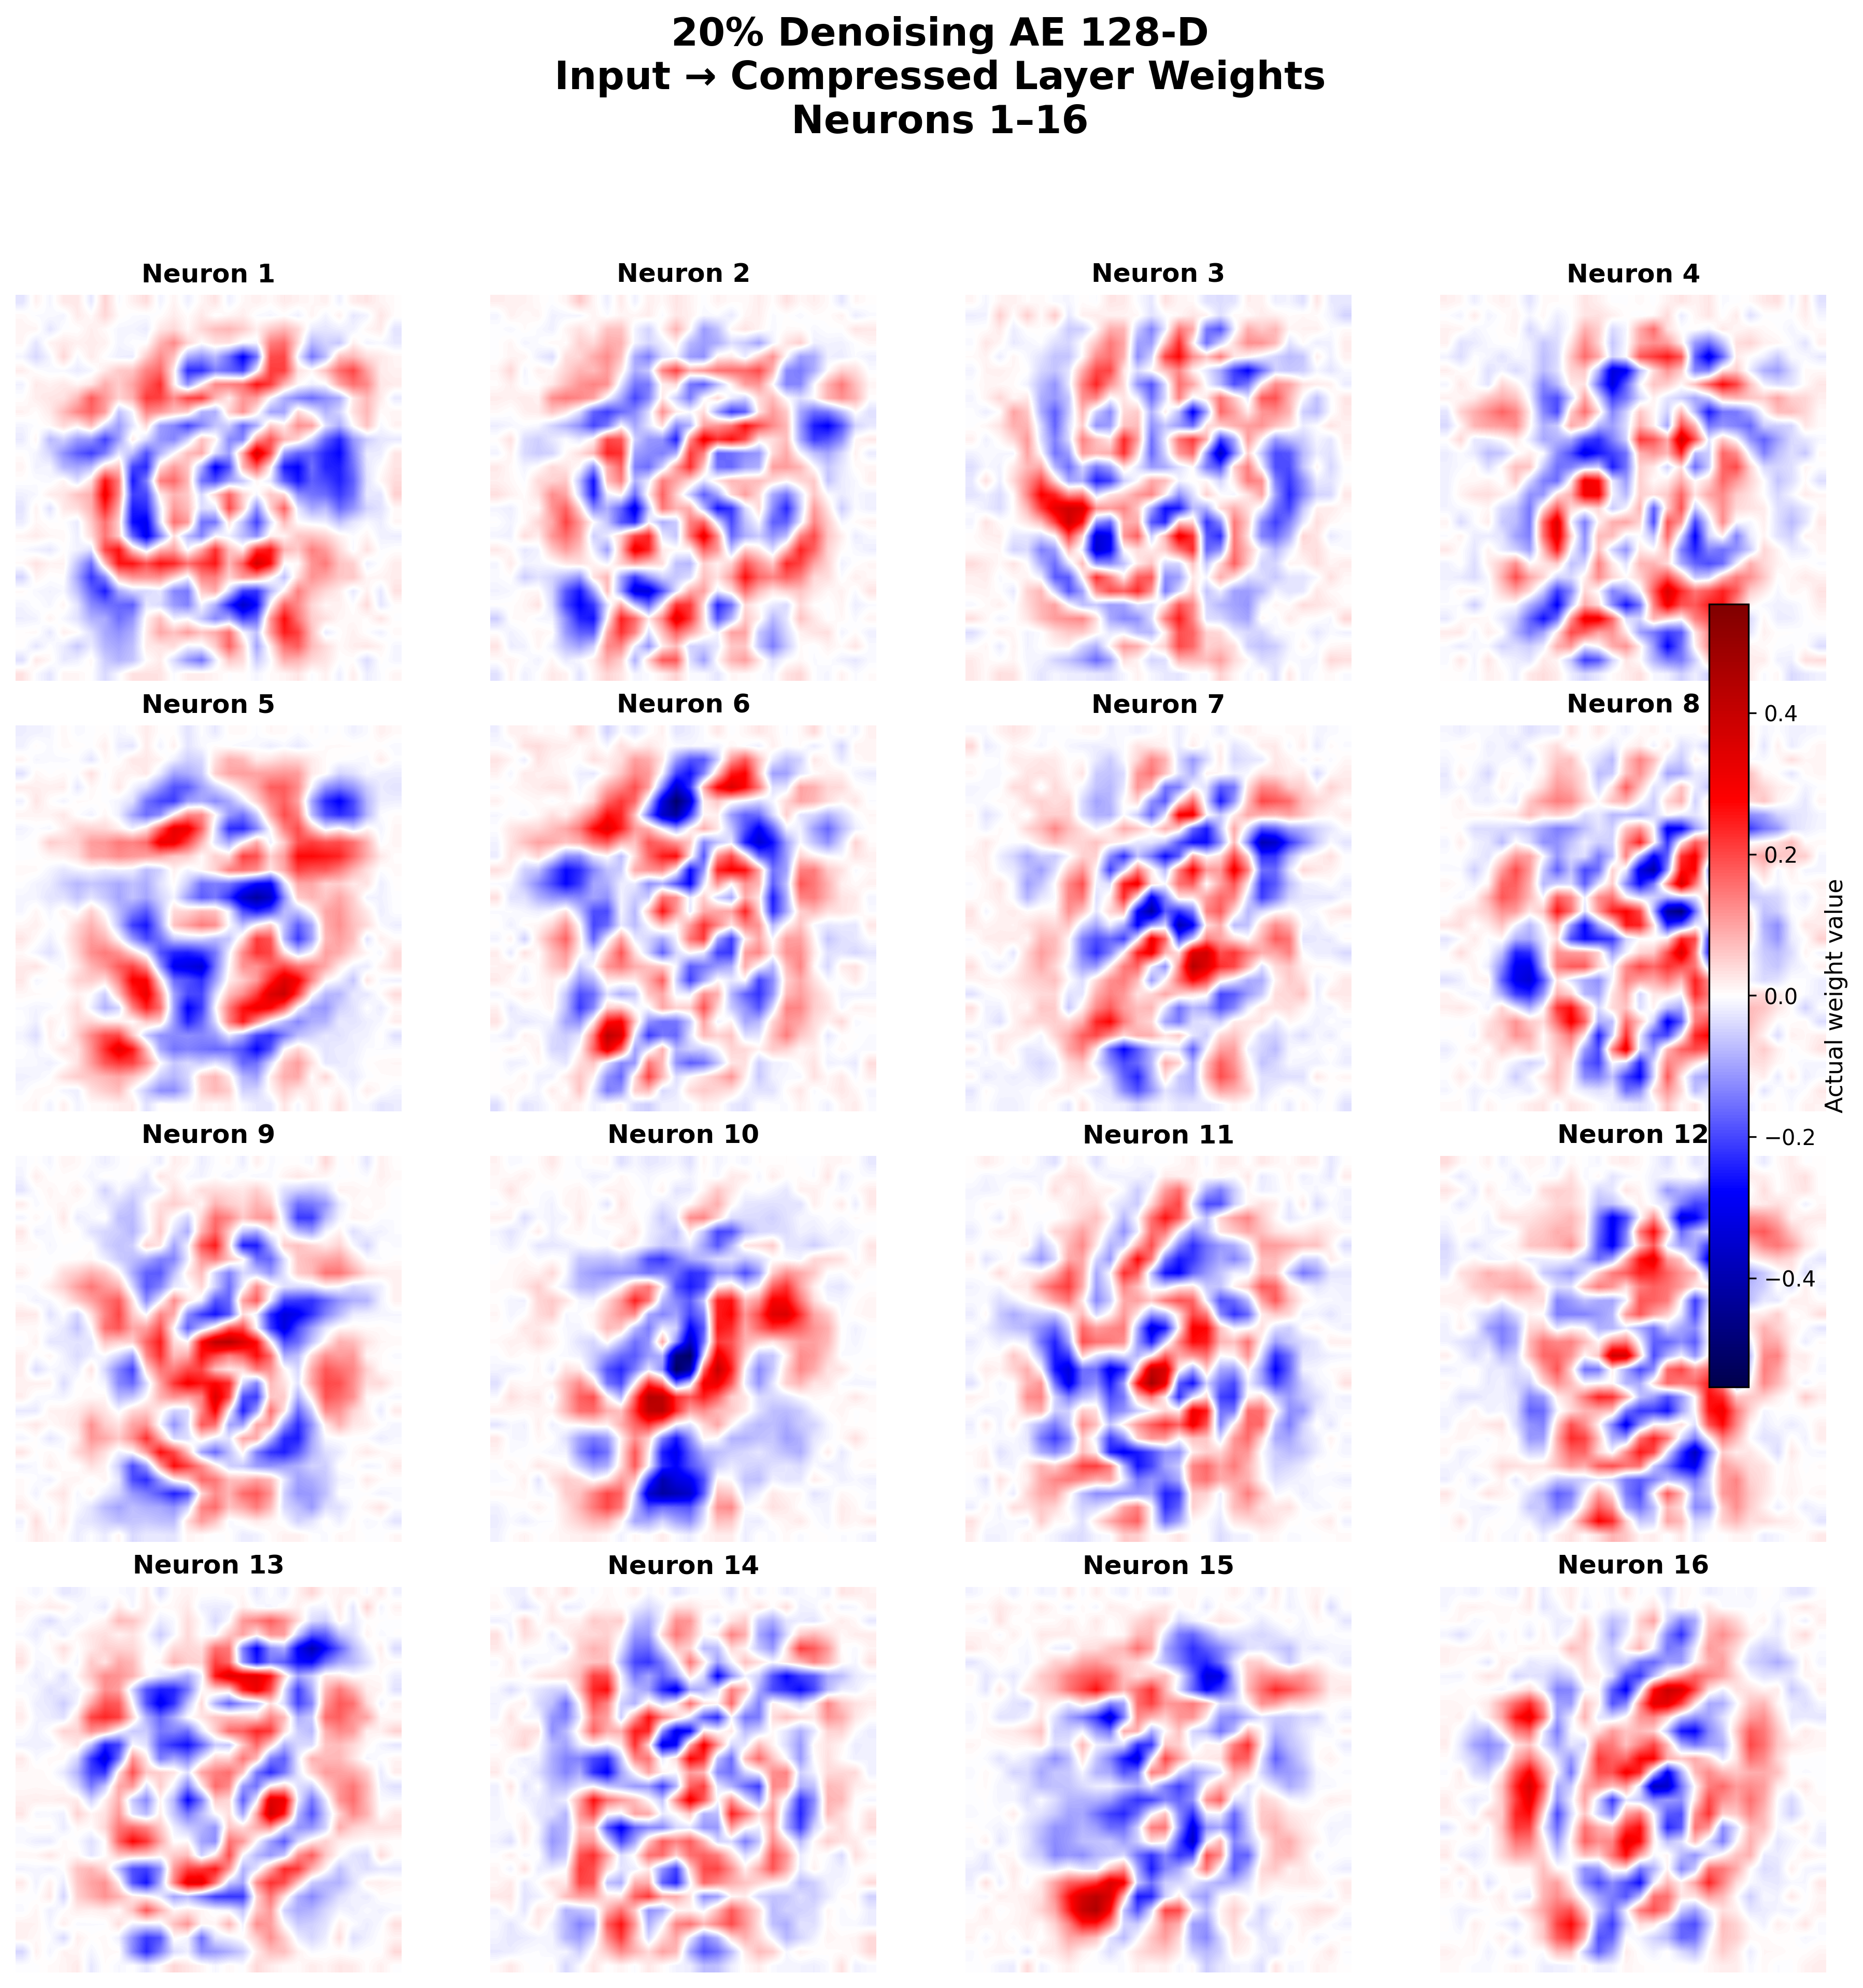
\includegraphics[width=0.99\linewidth,height=0.72\textheight,keepaspectratio]{figures/task6/20_pct_dae/neurons_001_016.png}
\caption{Input-to-bottleneck weight visualization for neurons 1--16.}
\label{fig:task6_9}
\end{figure}

\begin{figure}[H]
\centering
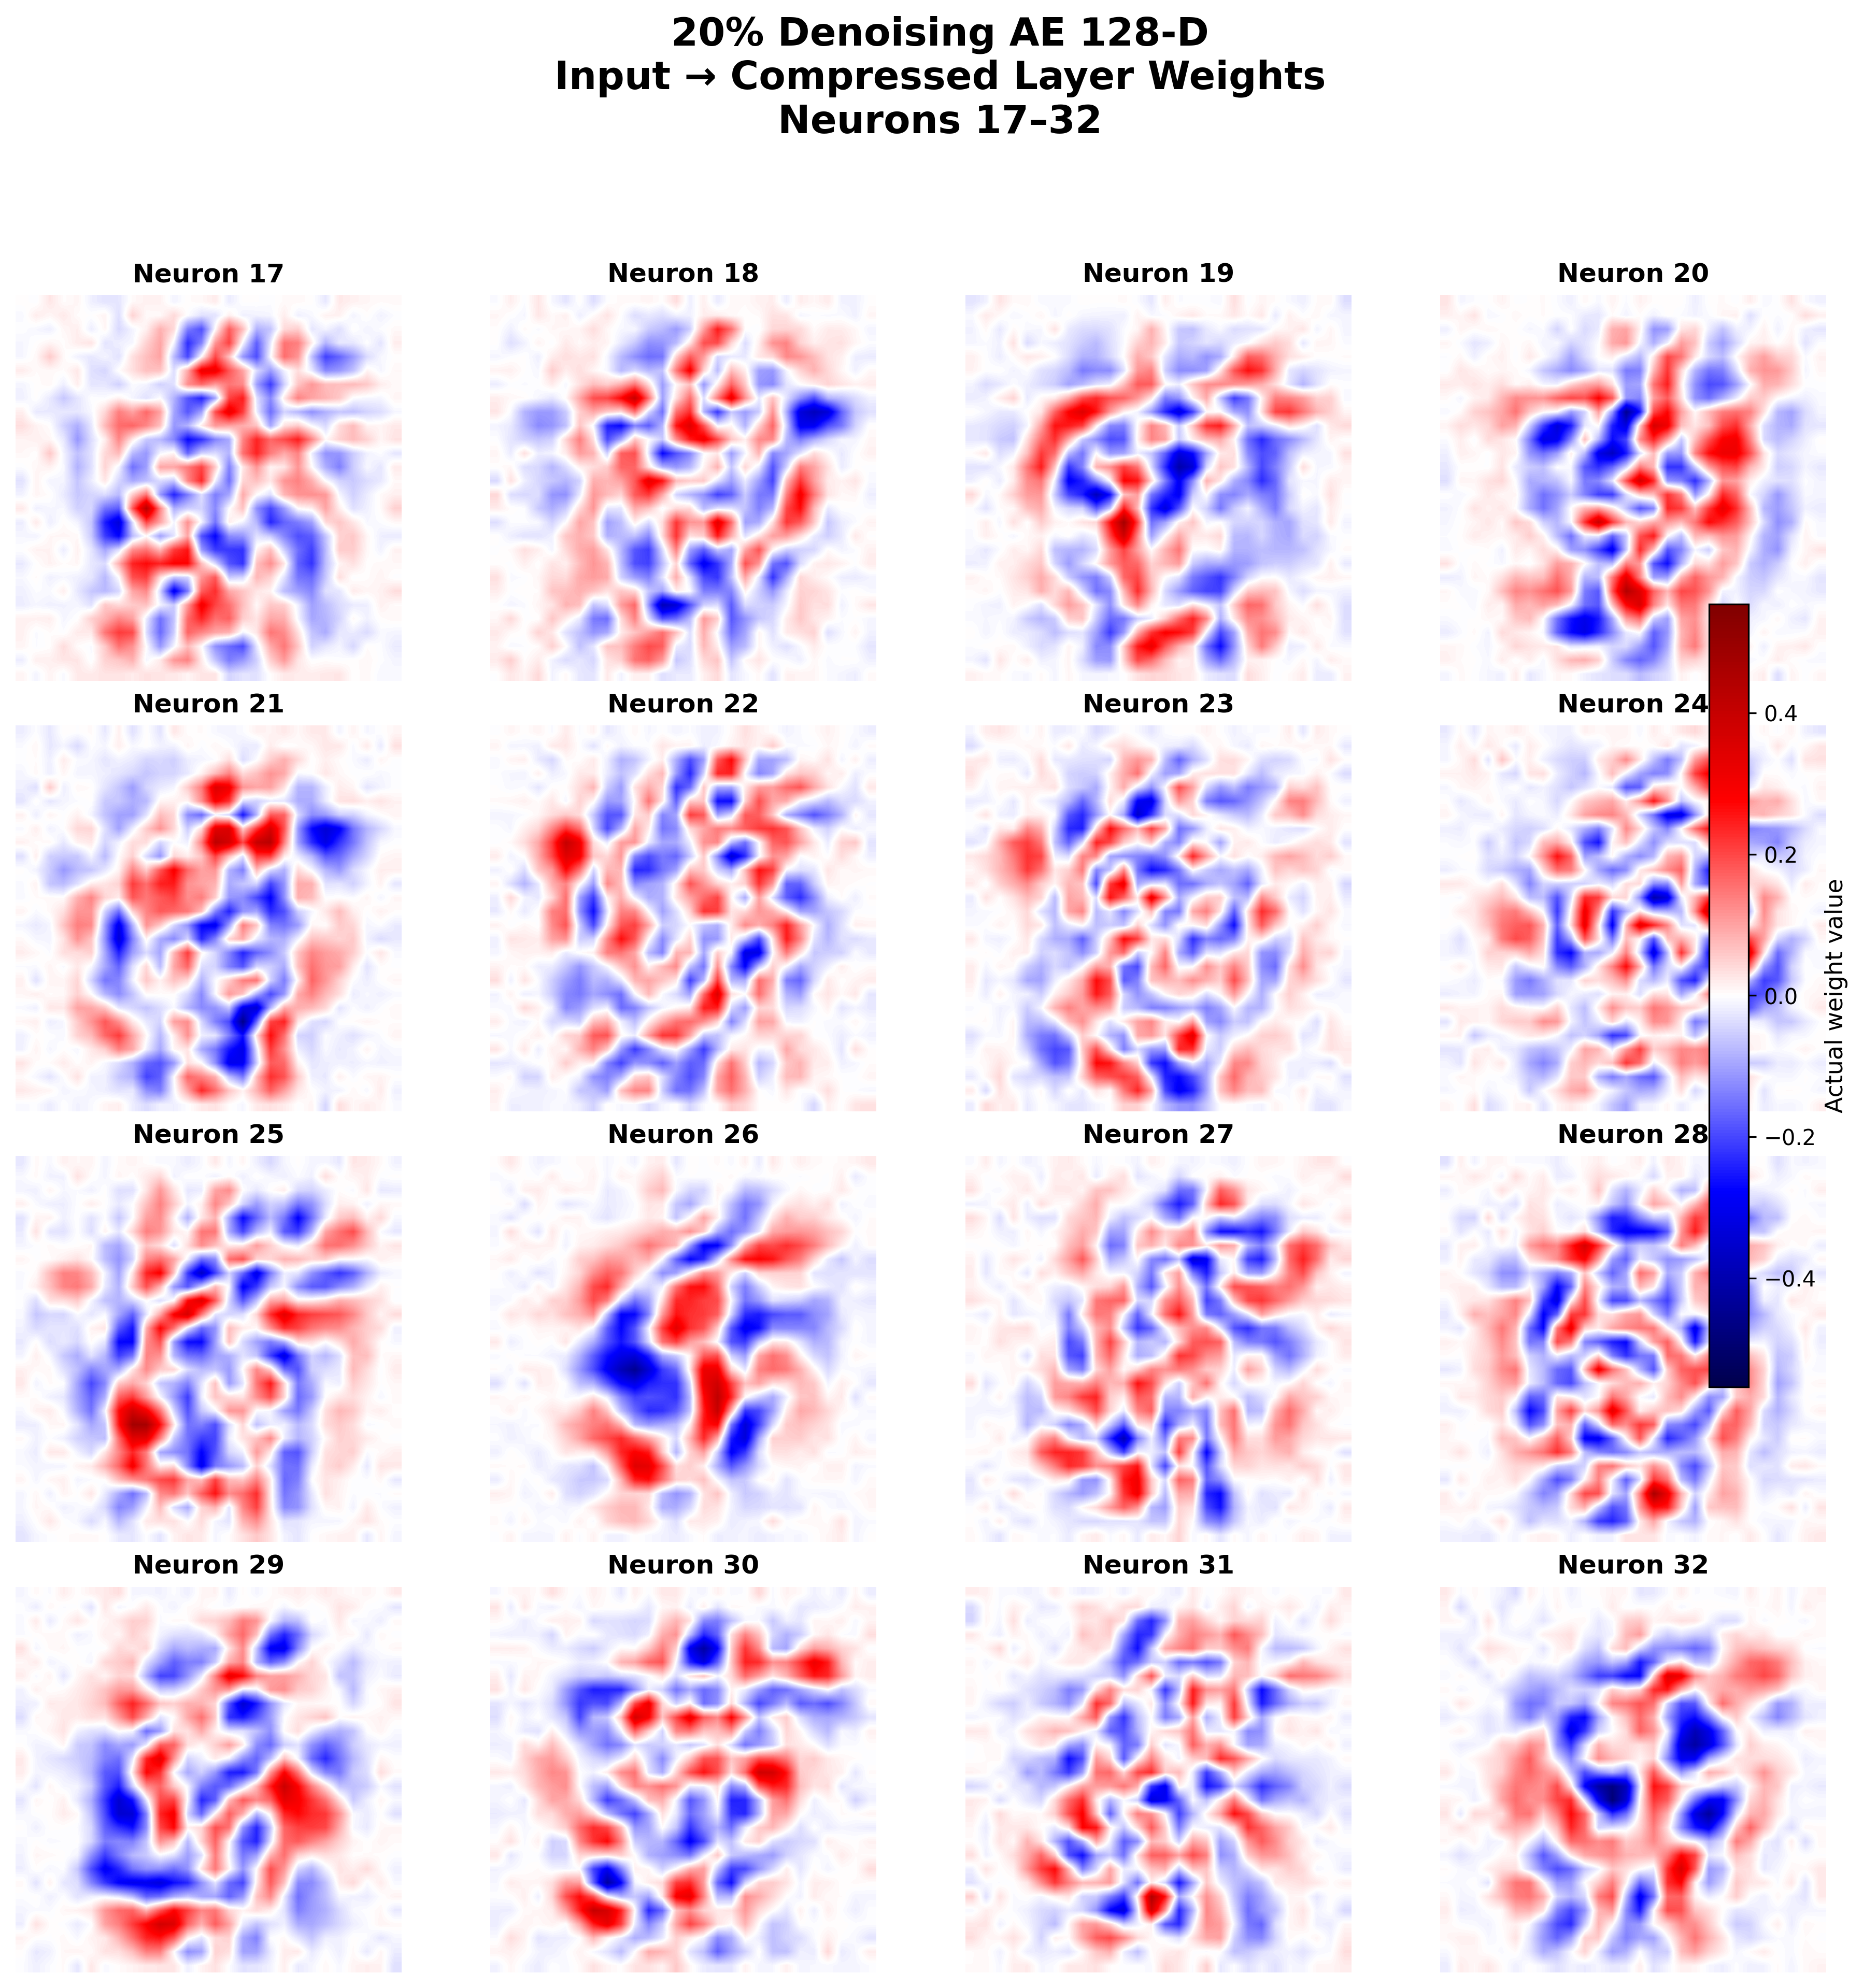
\includegraphics[width=0.99\linewidth,height=0.72\textheight,keepaspectratio]{figures/task6/20_pct_dae/neurons_017_032.png}
\caption{Input-to-bottleneck weight visualization for neurons 17--32.}
\label{fig:task6_10}
\end{figure}

\begin{figure}[H]
\centering
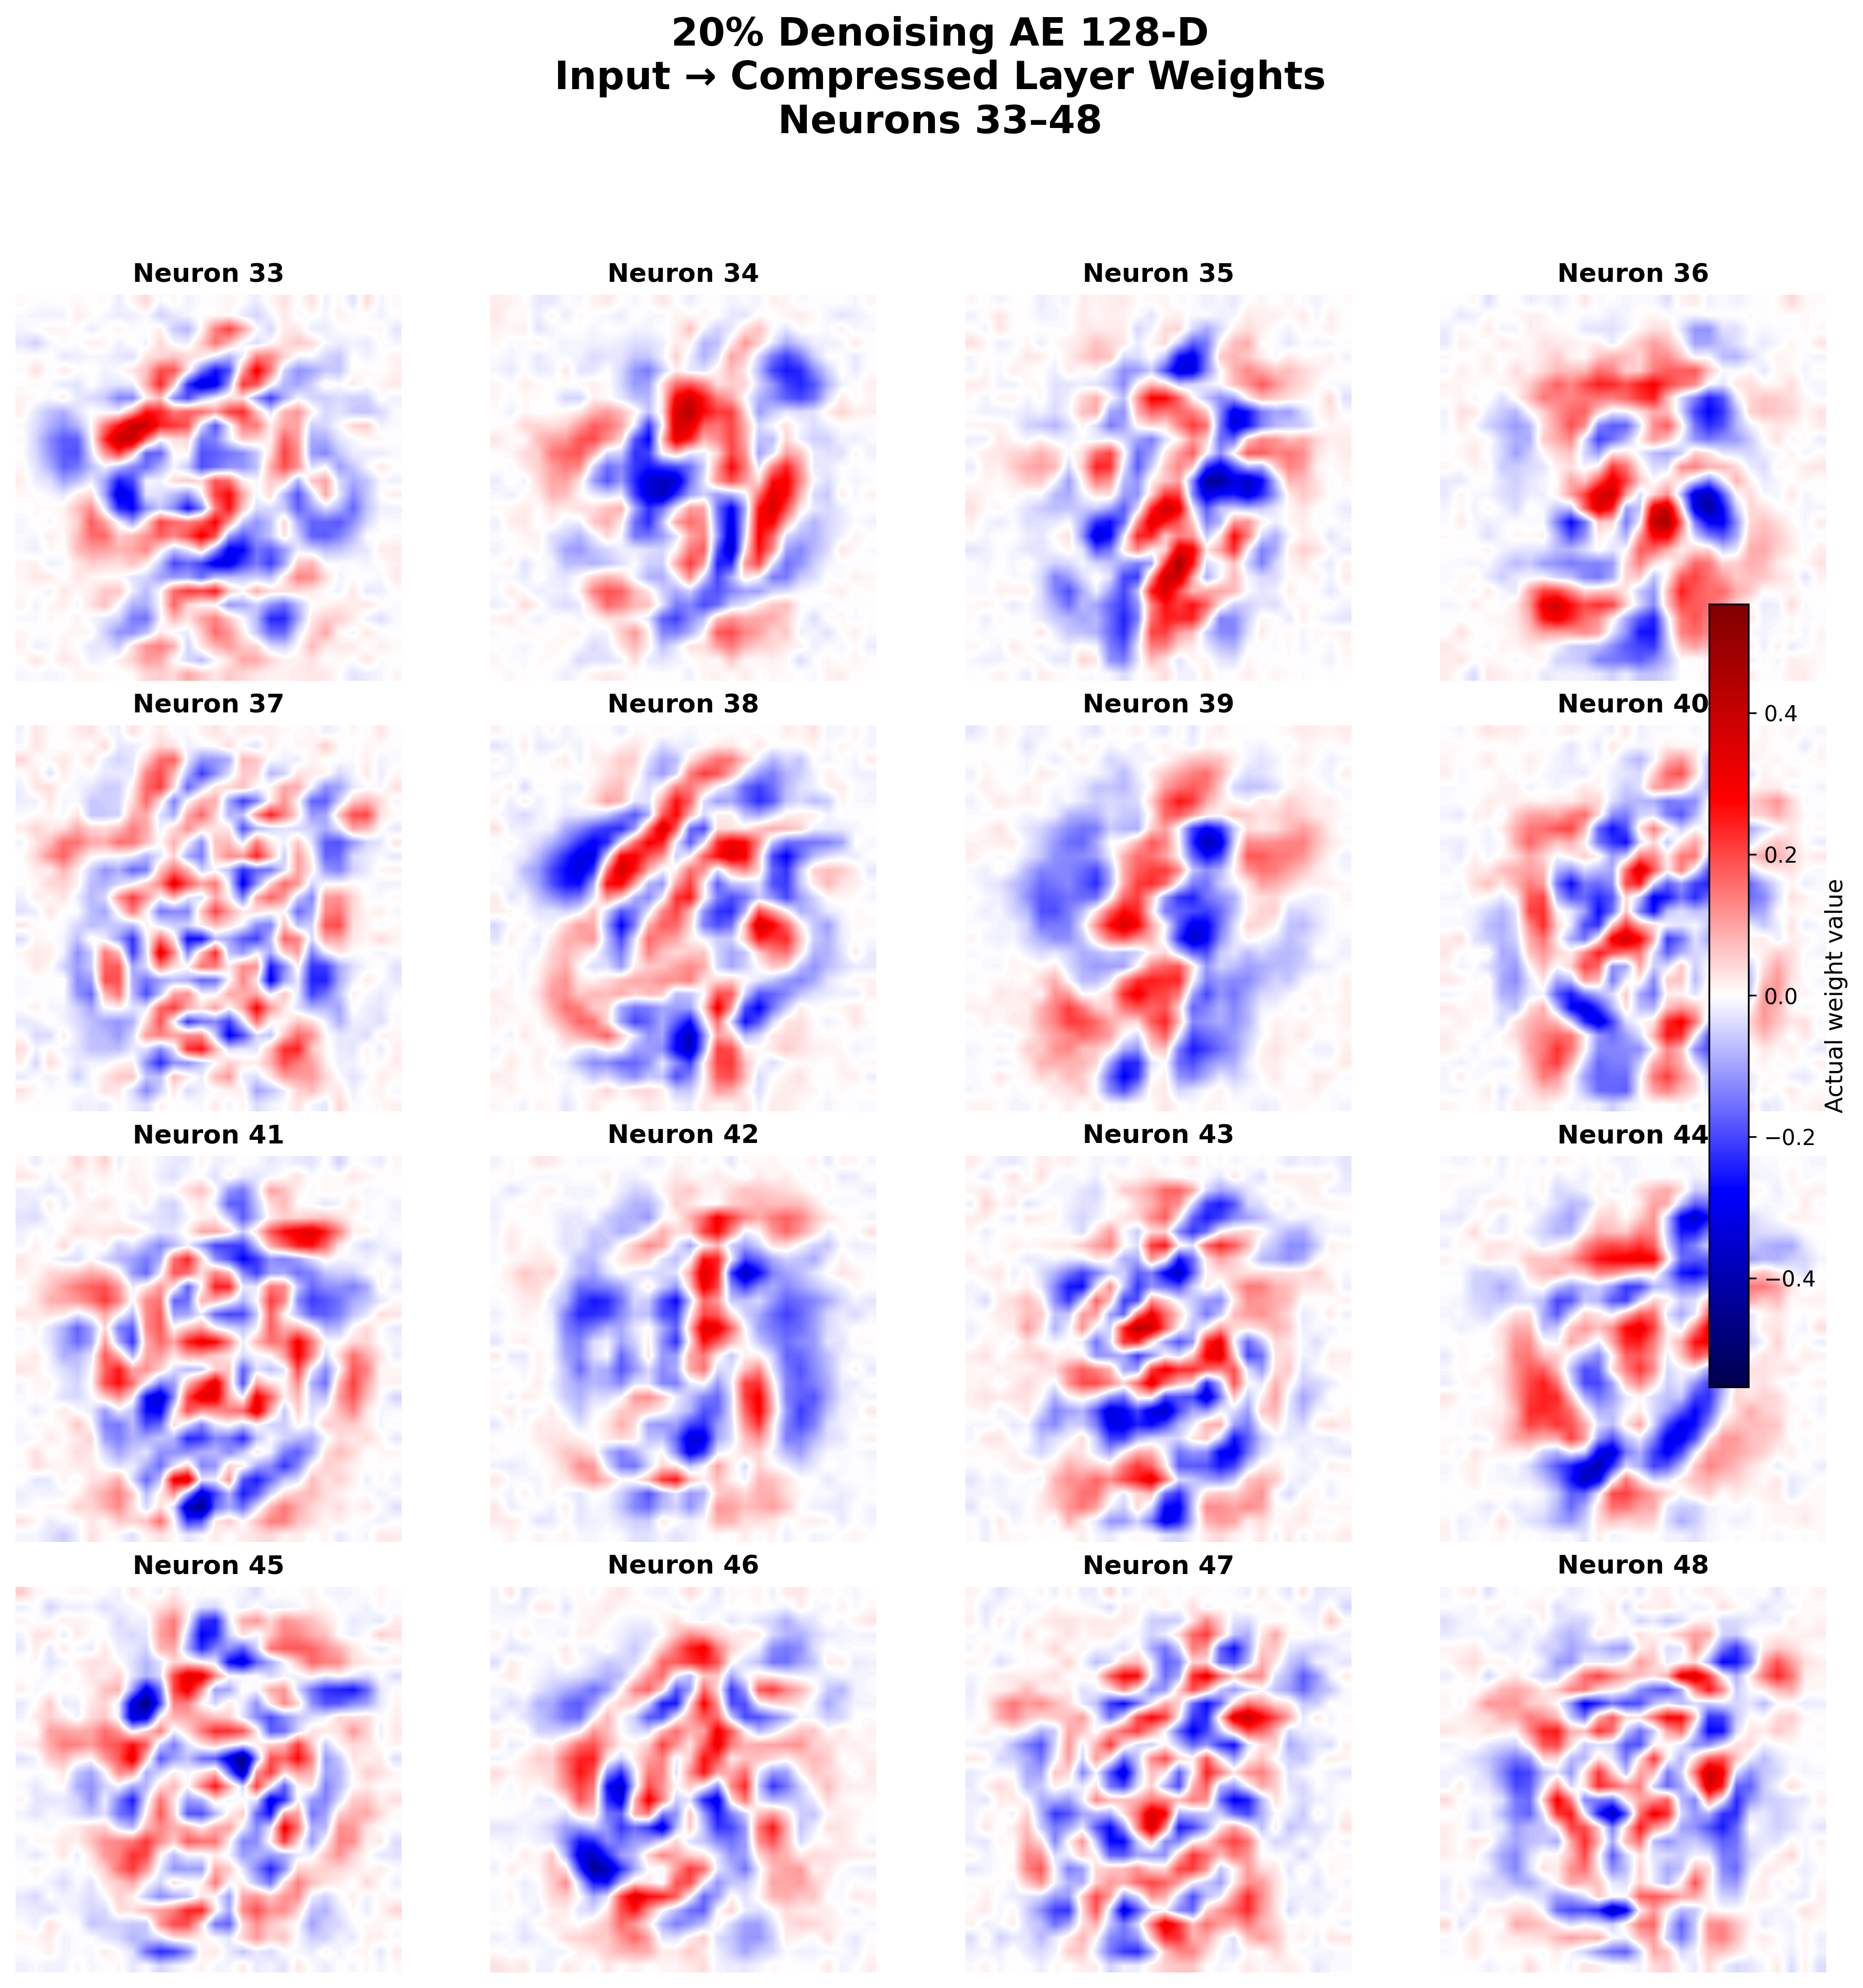
\includegraphics[width=0.99\linewidth,height=0.72\textheight,keepaspectratio]{figures/task6/20_pct_dae/neurons_033_048.png}
\caption{Input-to-bottleneck weight visualization for neurons 33--48.}
\label{fig:task6_11}
\end{figure}

\begin{figure}[H]
\centering
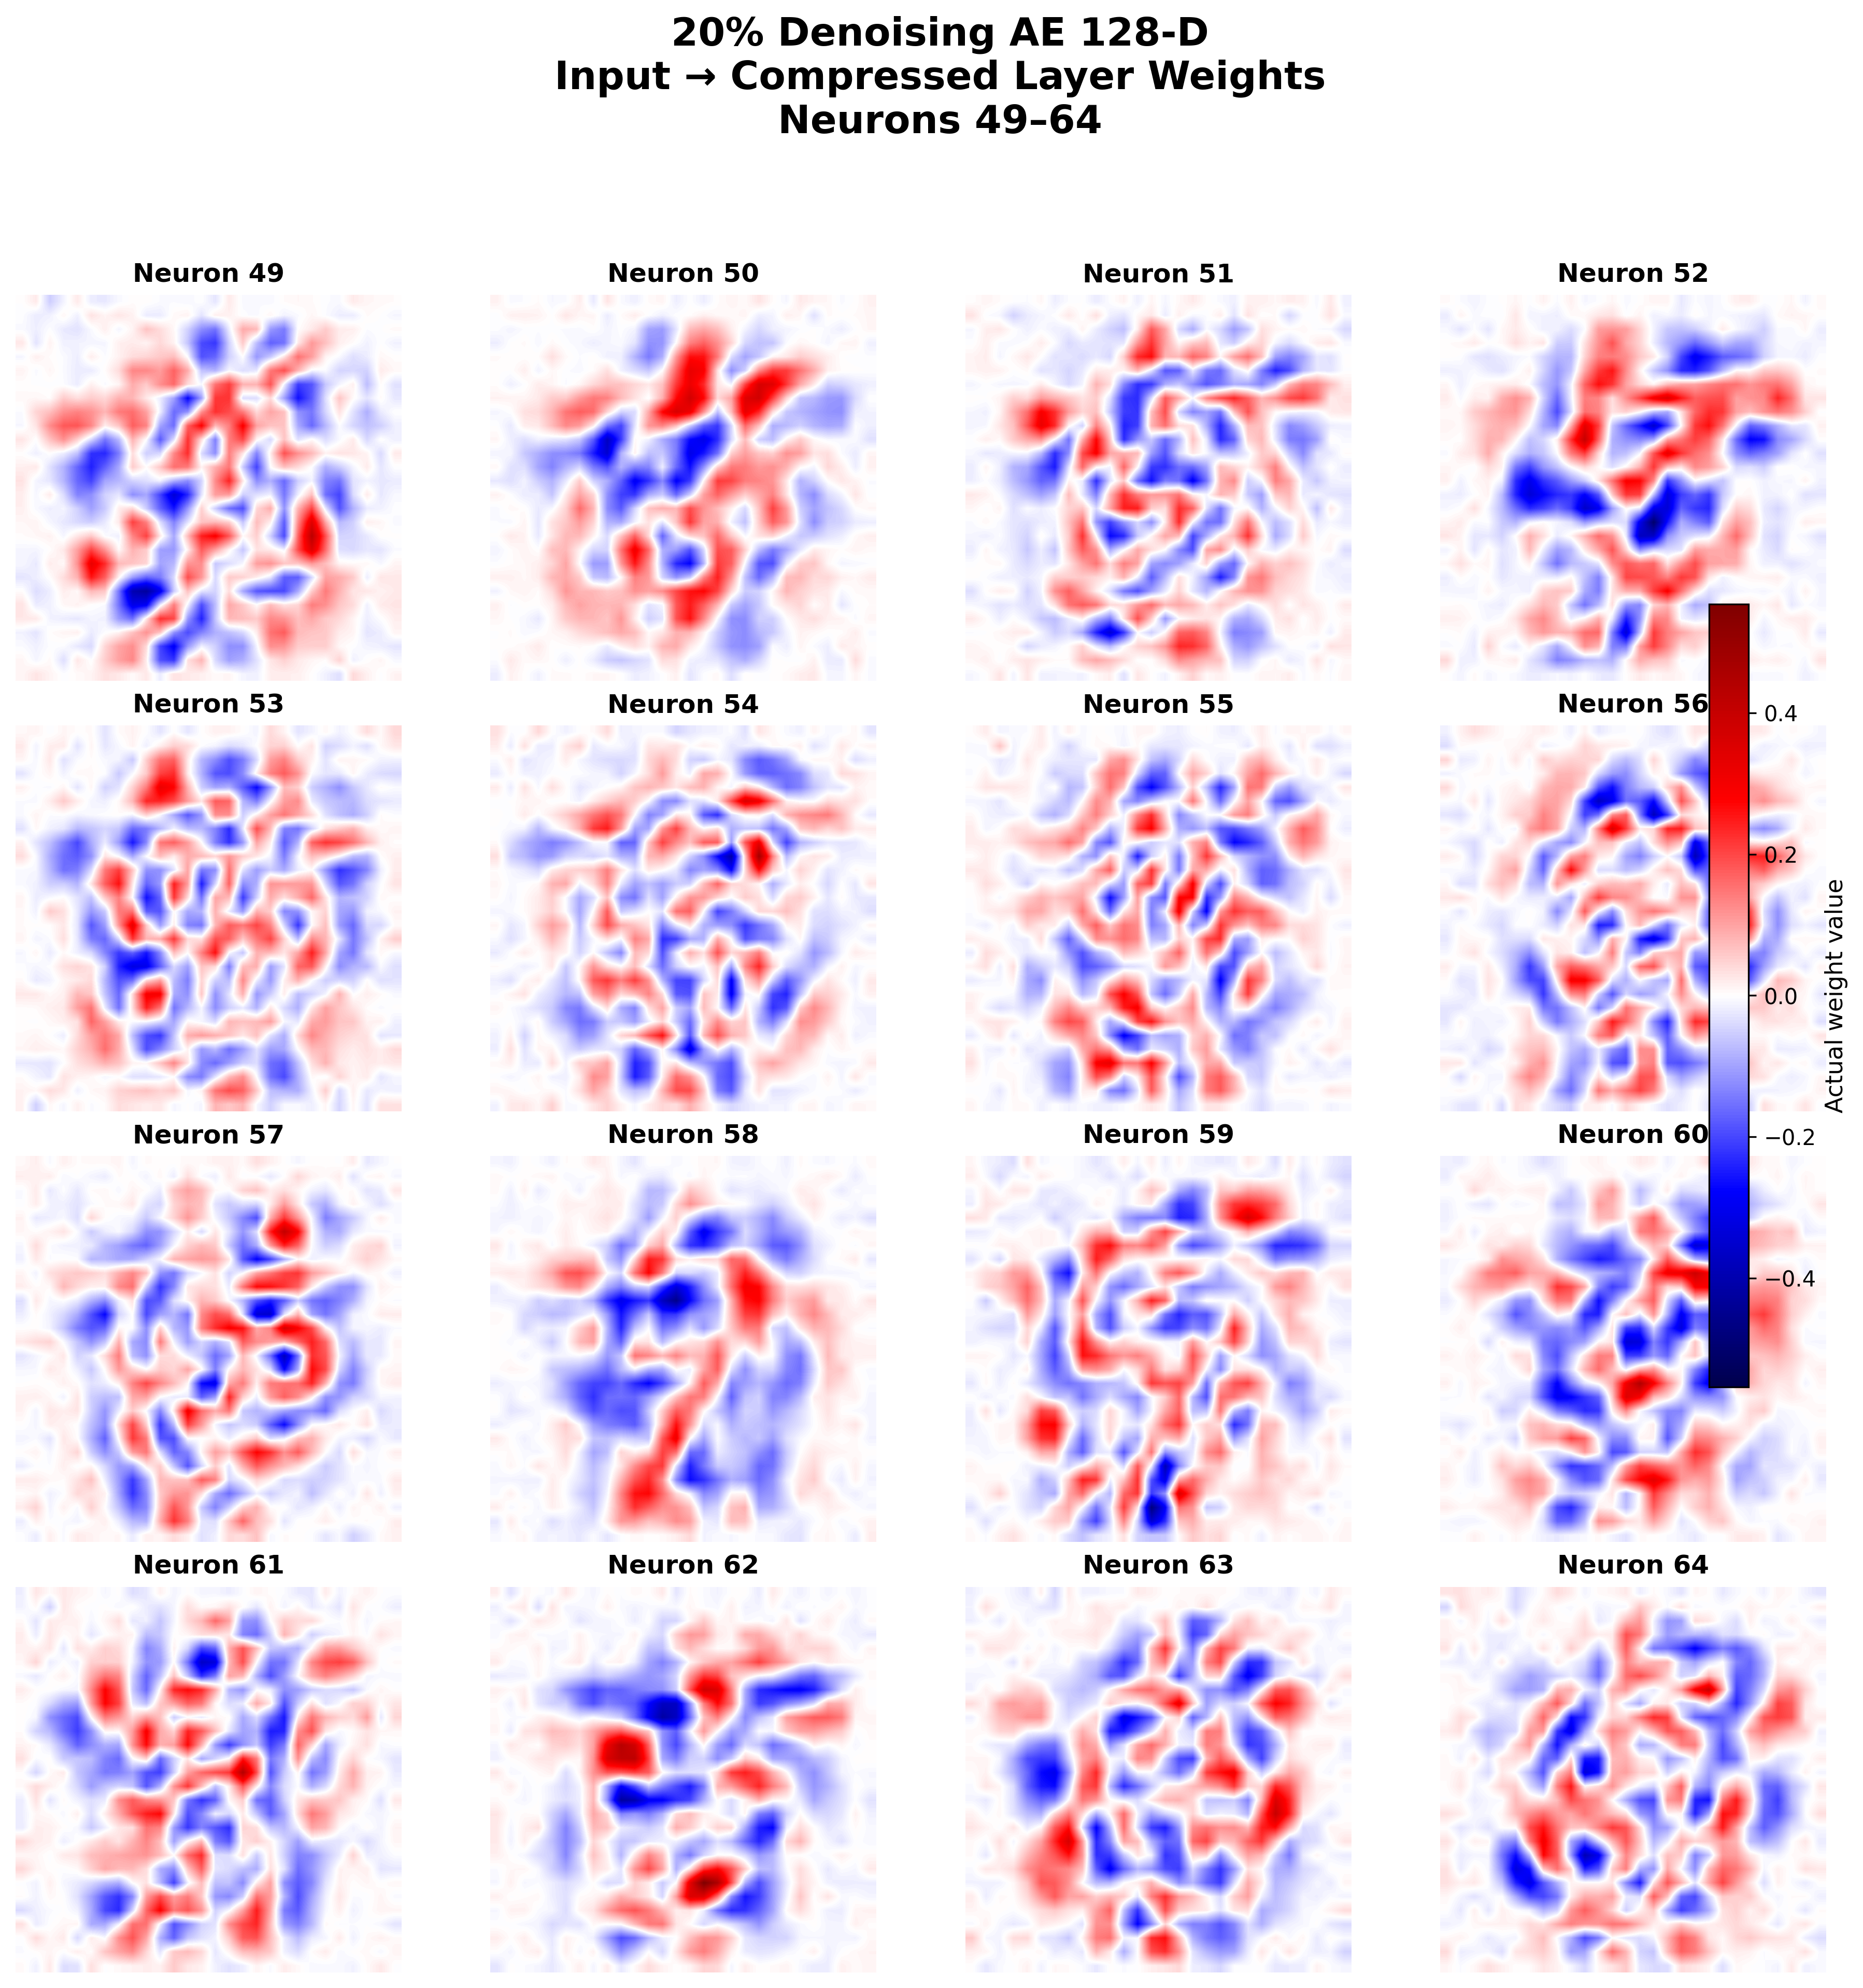
\includegraphics[width=0.99\linewidth,height=0.72\textheight,keepaspectratio]{figures/task6/20_pct_dae/neurons_049_064.png}
\caption{Input-to-bottleneck weight visualization for neurons 49--64.}
\label{fig:task6_12}
\end{figure}

\begin{figure}[H]
\centering
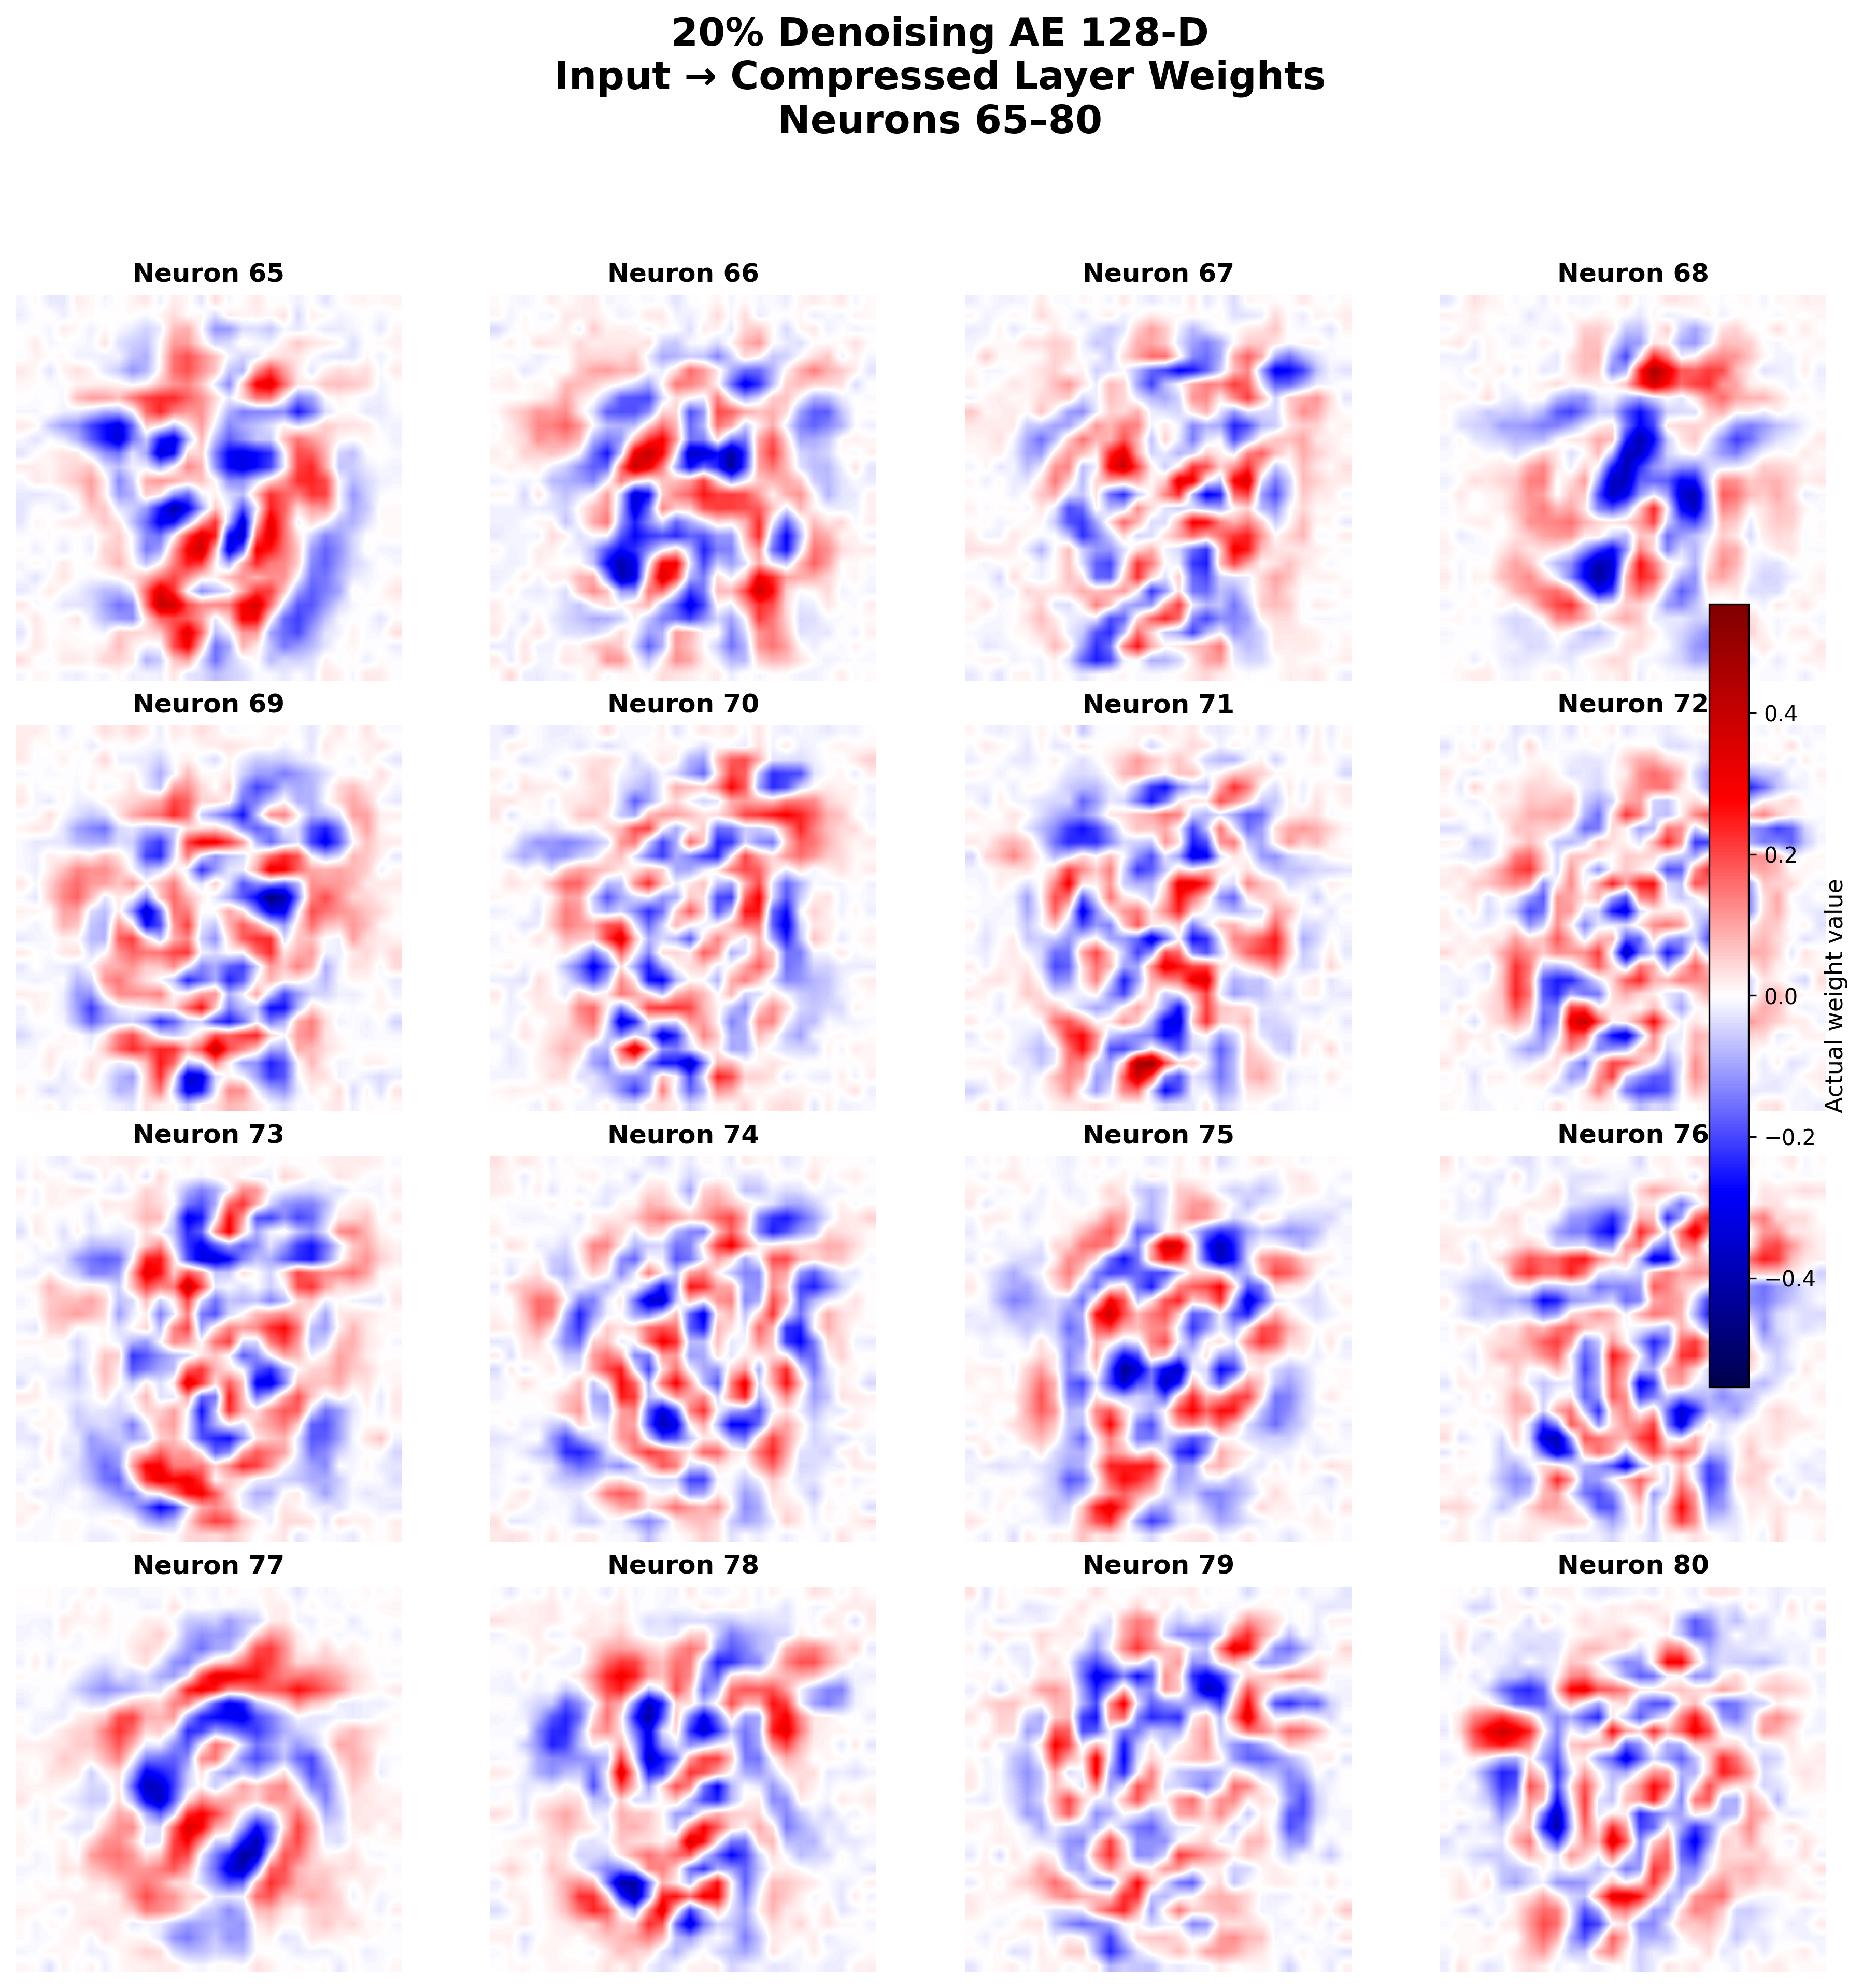
\includegraphics[width=0.99\linewidth,height=0.72\textheight,keepaspectratio]{figures/task6/20_pct_dae/neurons_065_080.png}
\caption{Input-to-bottleneck weight visualization for neurons 65--80.}
\label{fig:task6_13}
\end{figure}

\begin{figure}[H]
\centering
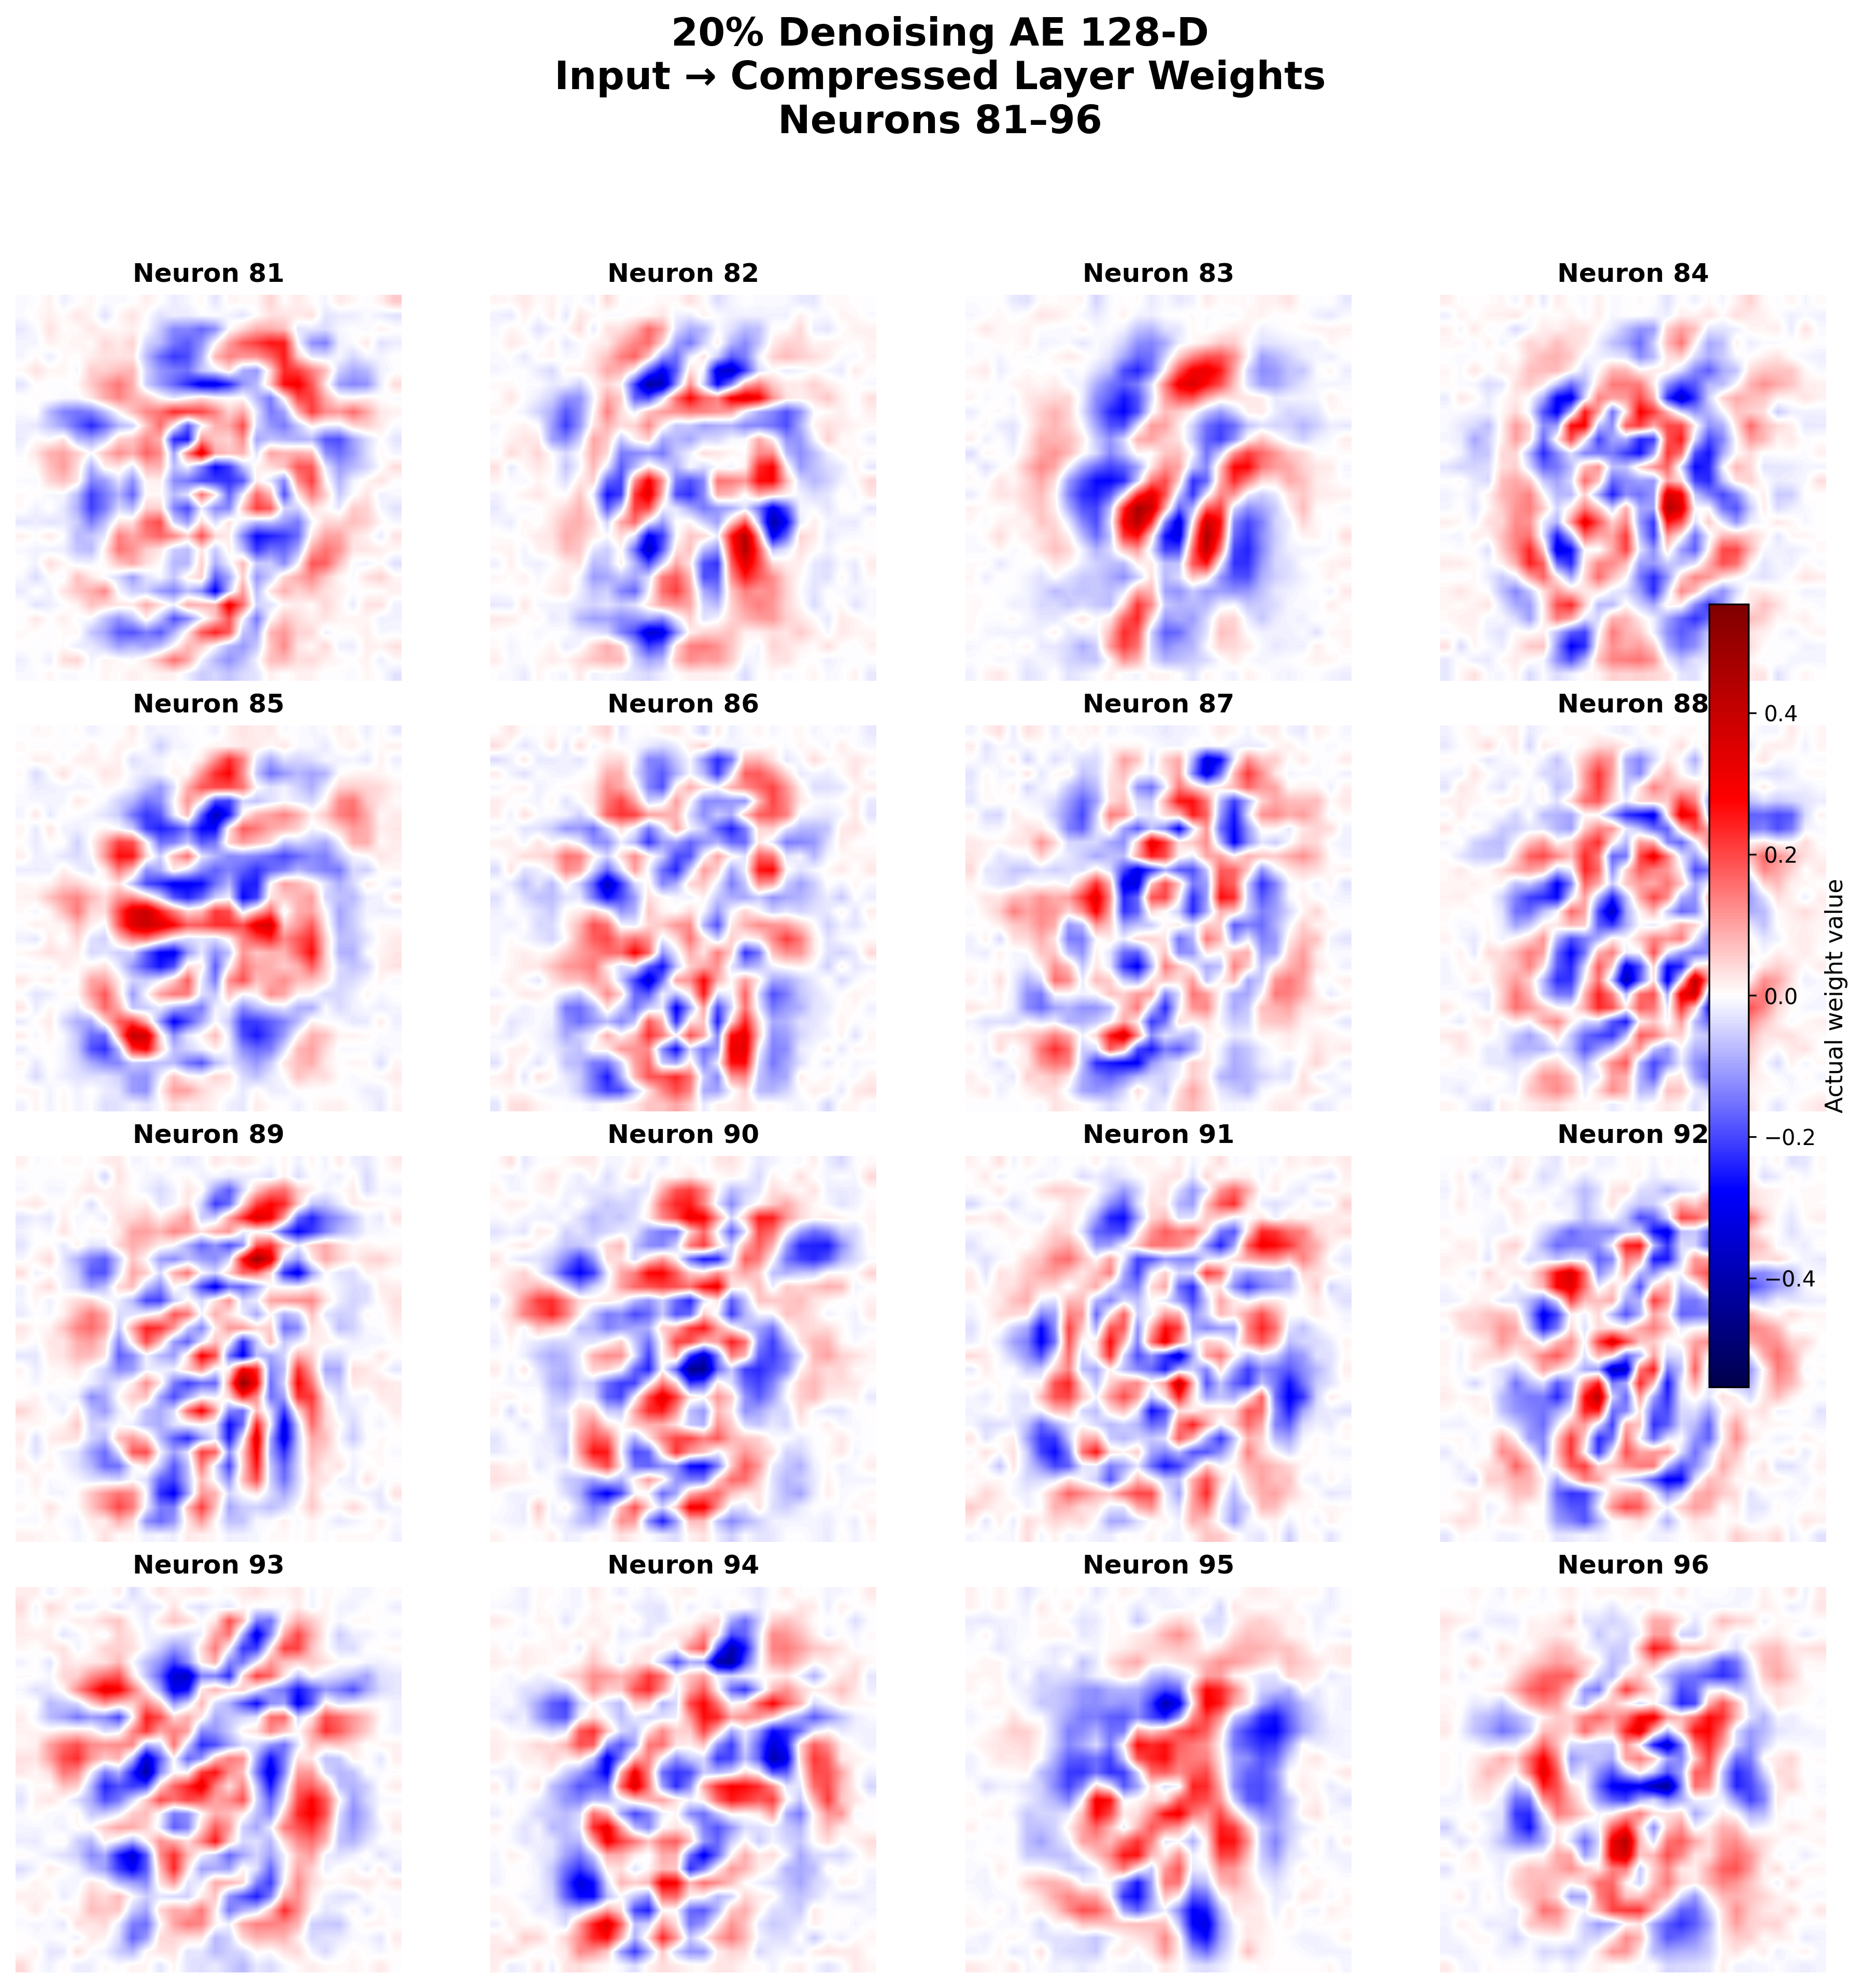
\includegraphics[width=0.99\linewidth,height=0.72\textheight,keepaspectratio]{figures/task6/20_pct_dae/neurons_081_096.png}
\caption{Input-to-bottleneck weight visualization for neurons 81--96.}
\label{fig:task6_14}
\end{figure}

\begin{figure}[H]
\centering
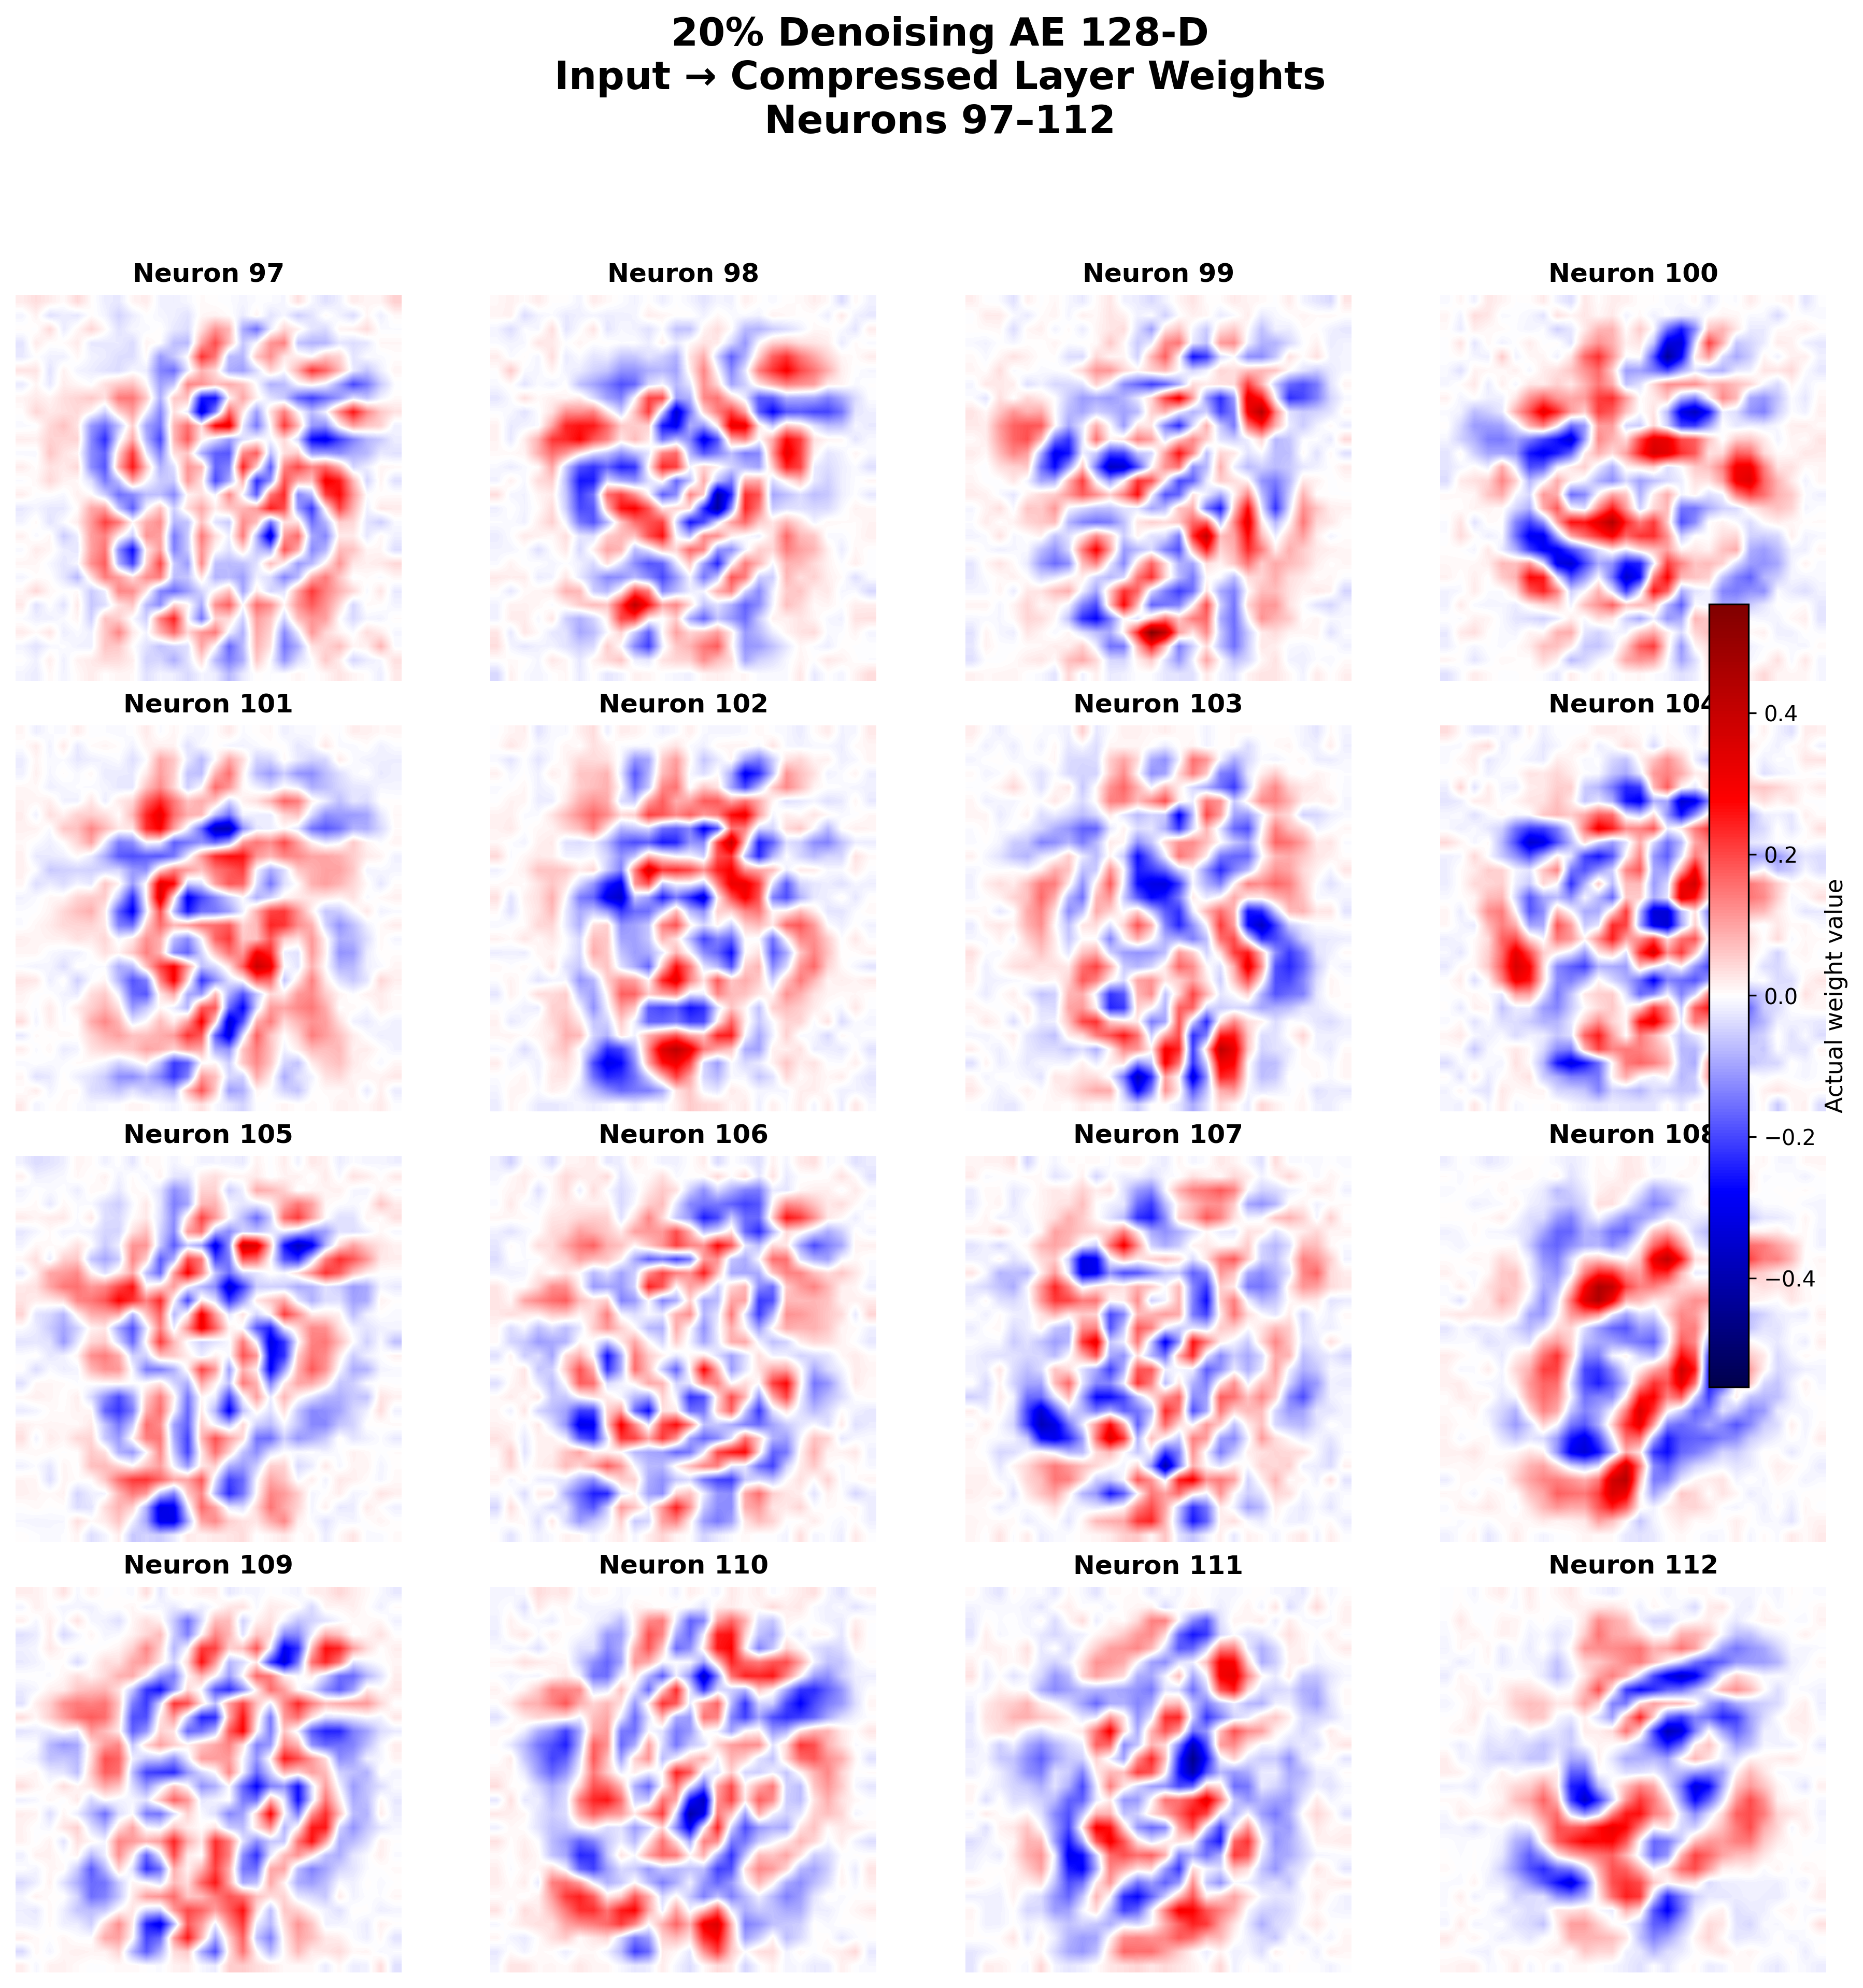
\includegraphics[width=0.99\linewidth,height=0.72\textheight,keepaspectratio]{figures/task6/20_pct_dae/neurons_097_112.png}
\caption{Input-to-bottleneck weight visualization for neurons 97--112.}
\label{fig:task6_15}
\end{figure}

\begin{figure}[H]
\centering
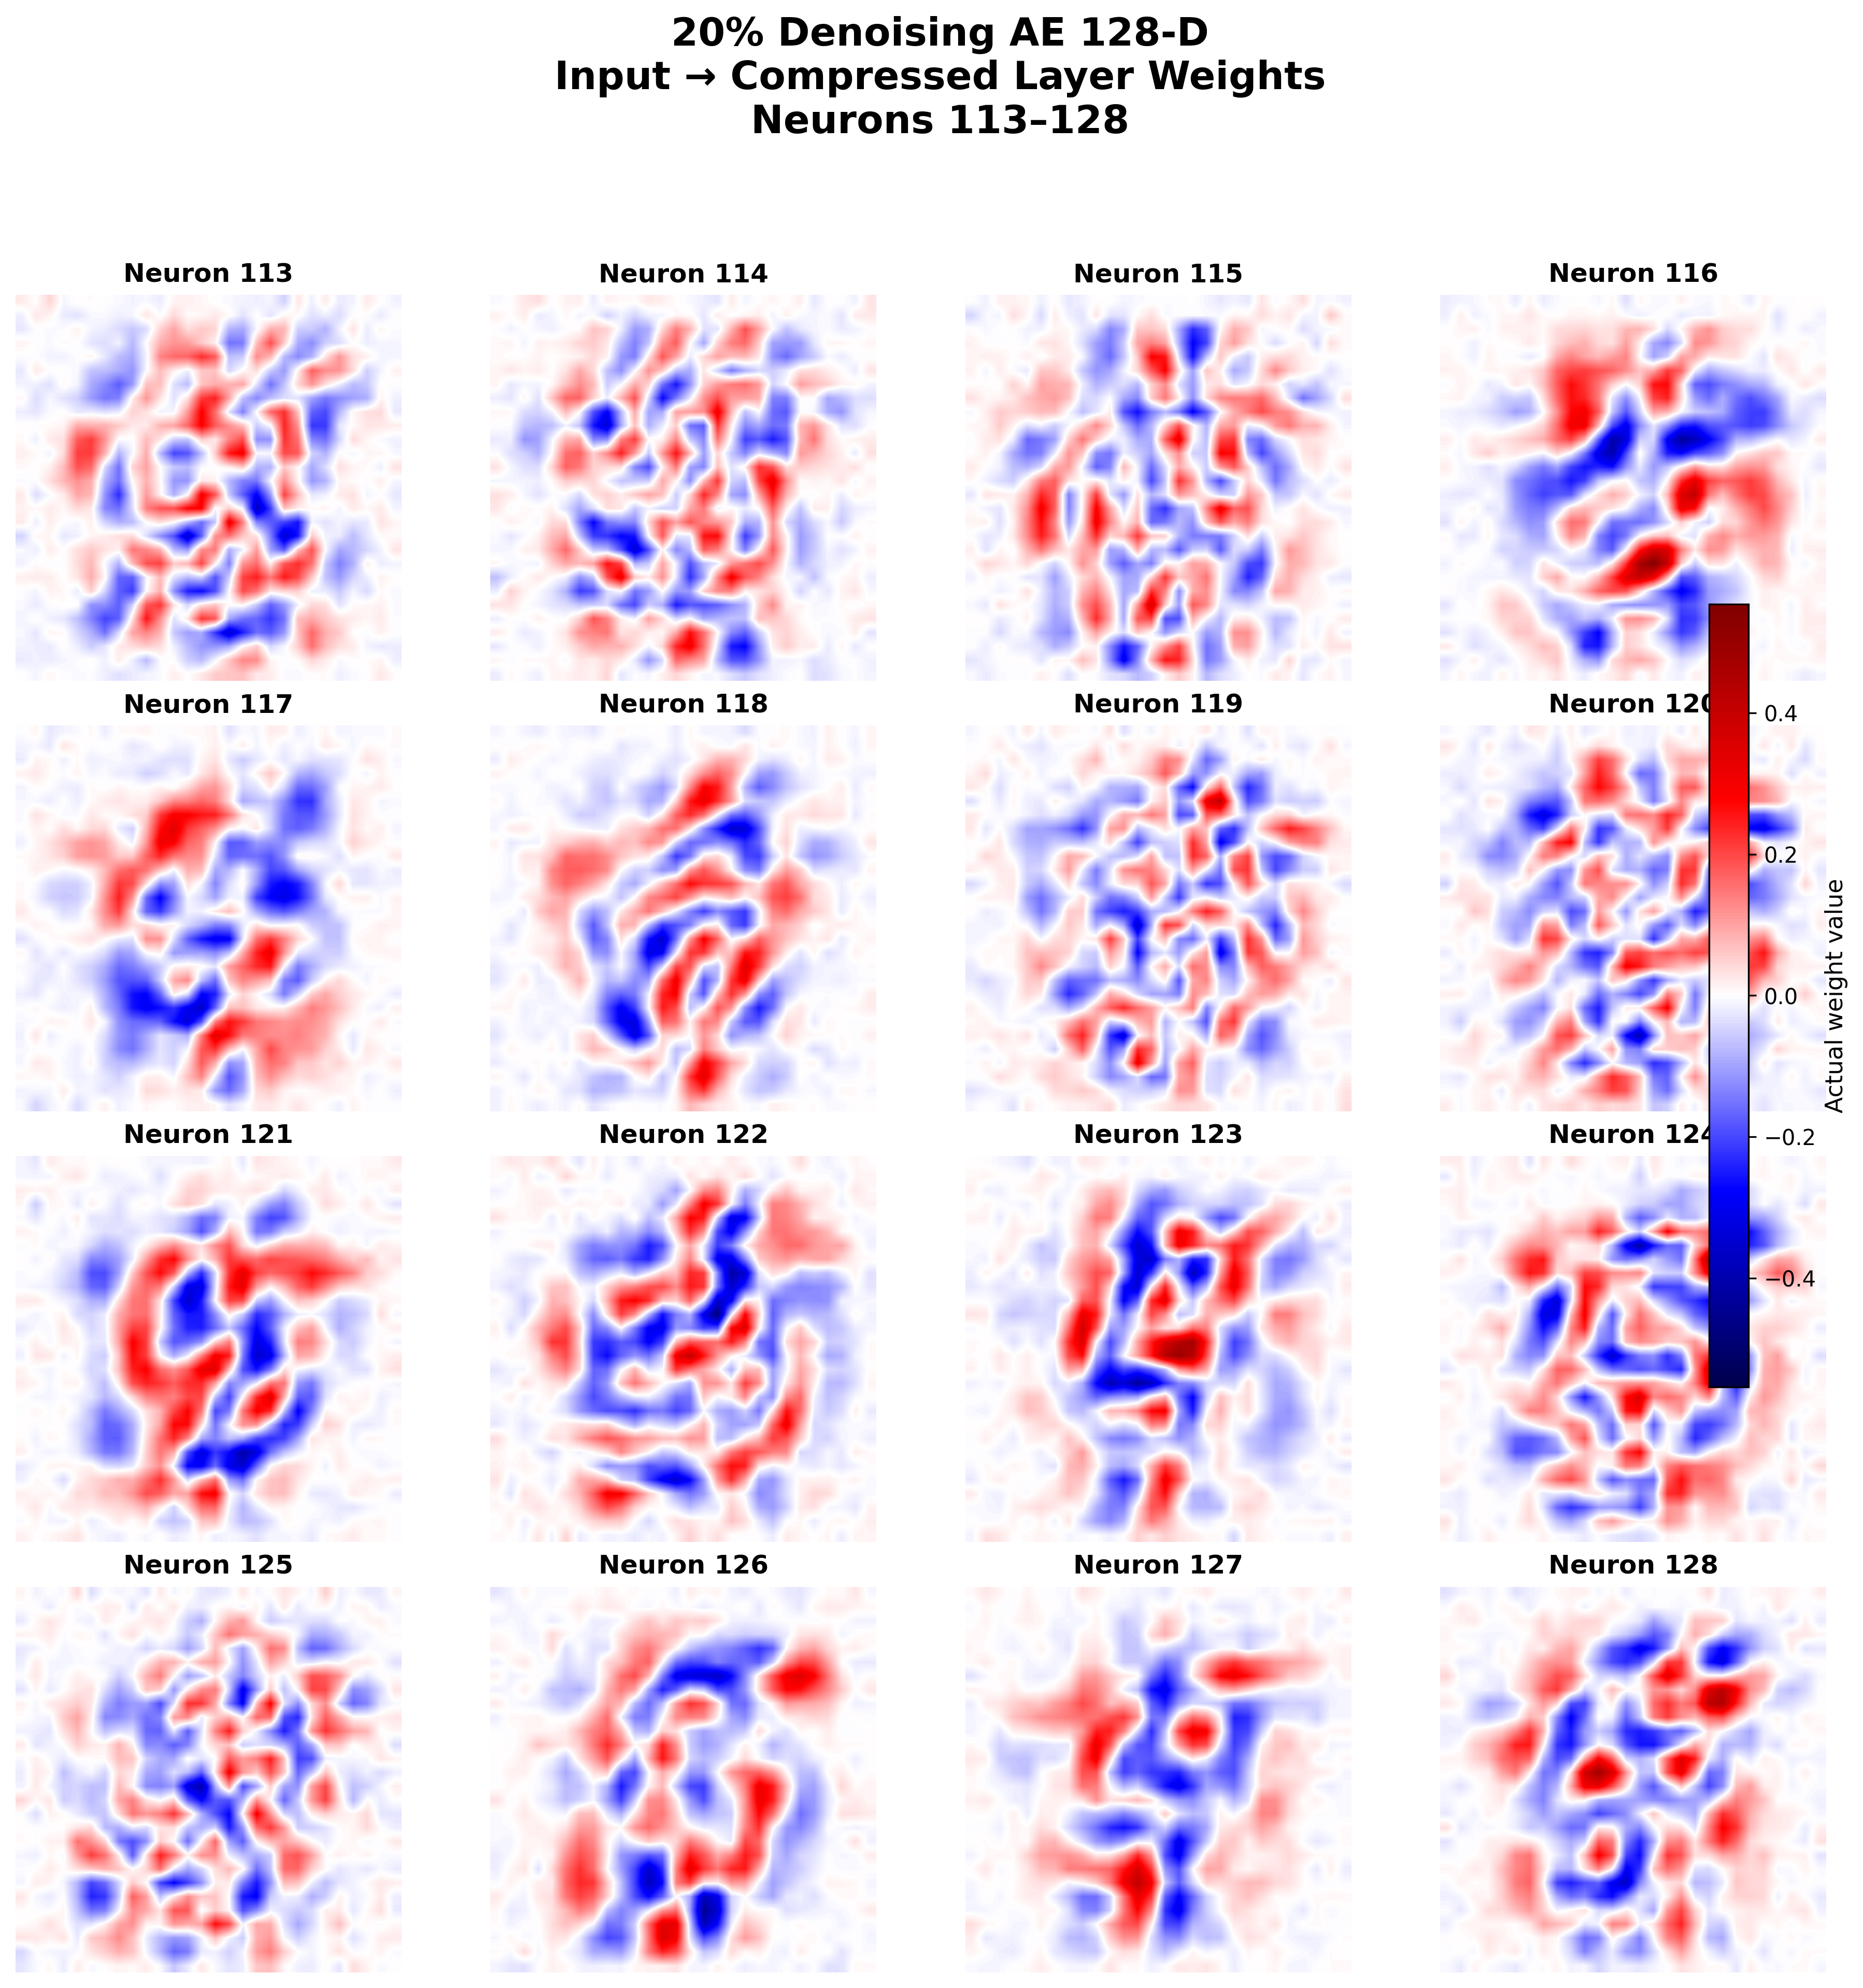
\includegraphics[width=0.99\linewidth,height=0.72\textheight,keepaspectratio]{figures/task6/20_pct_dae/neurons_113_128.png}
\caption{Input-to-bottleneck weight visualization for neurons 113--128.}
\label{fig:task6_16}
\end{figure}

\begin{figure}[H]
\centering
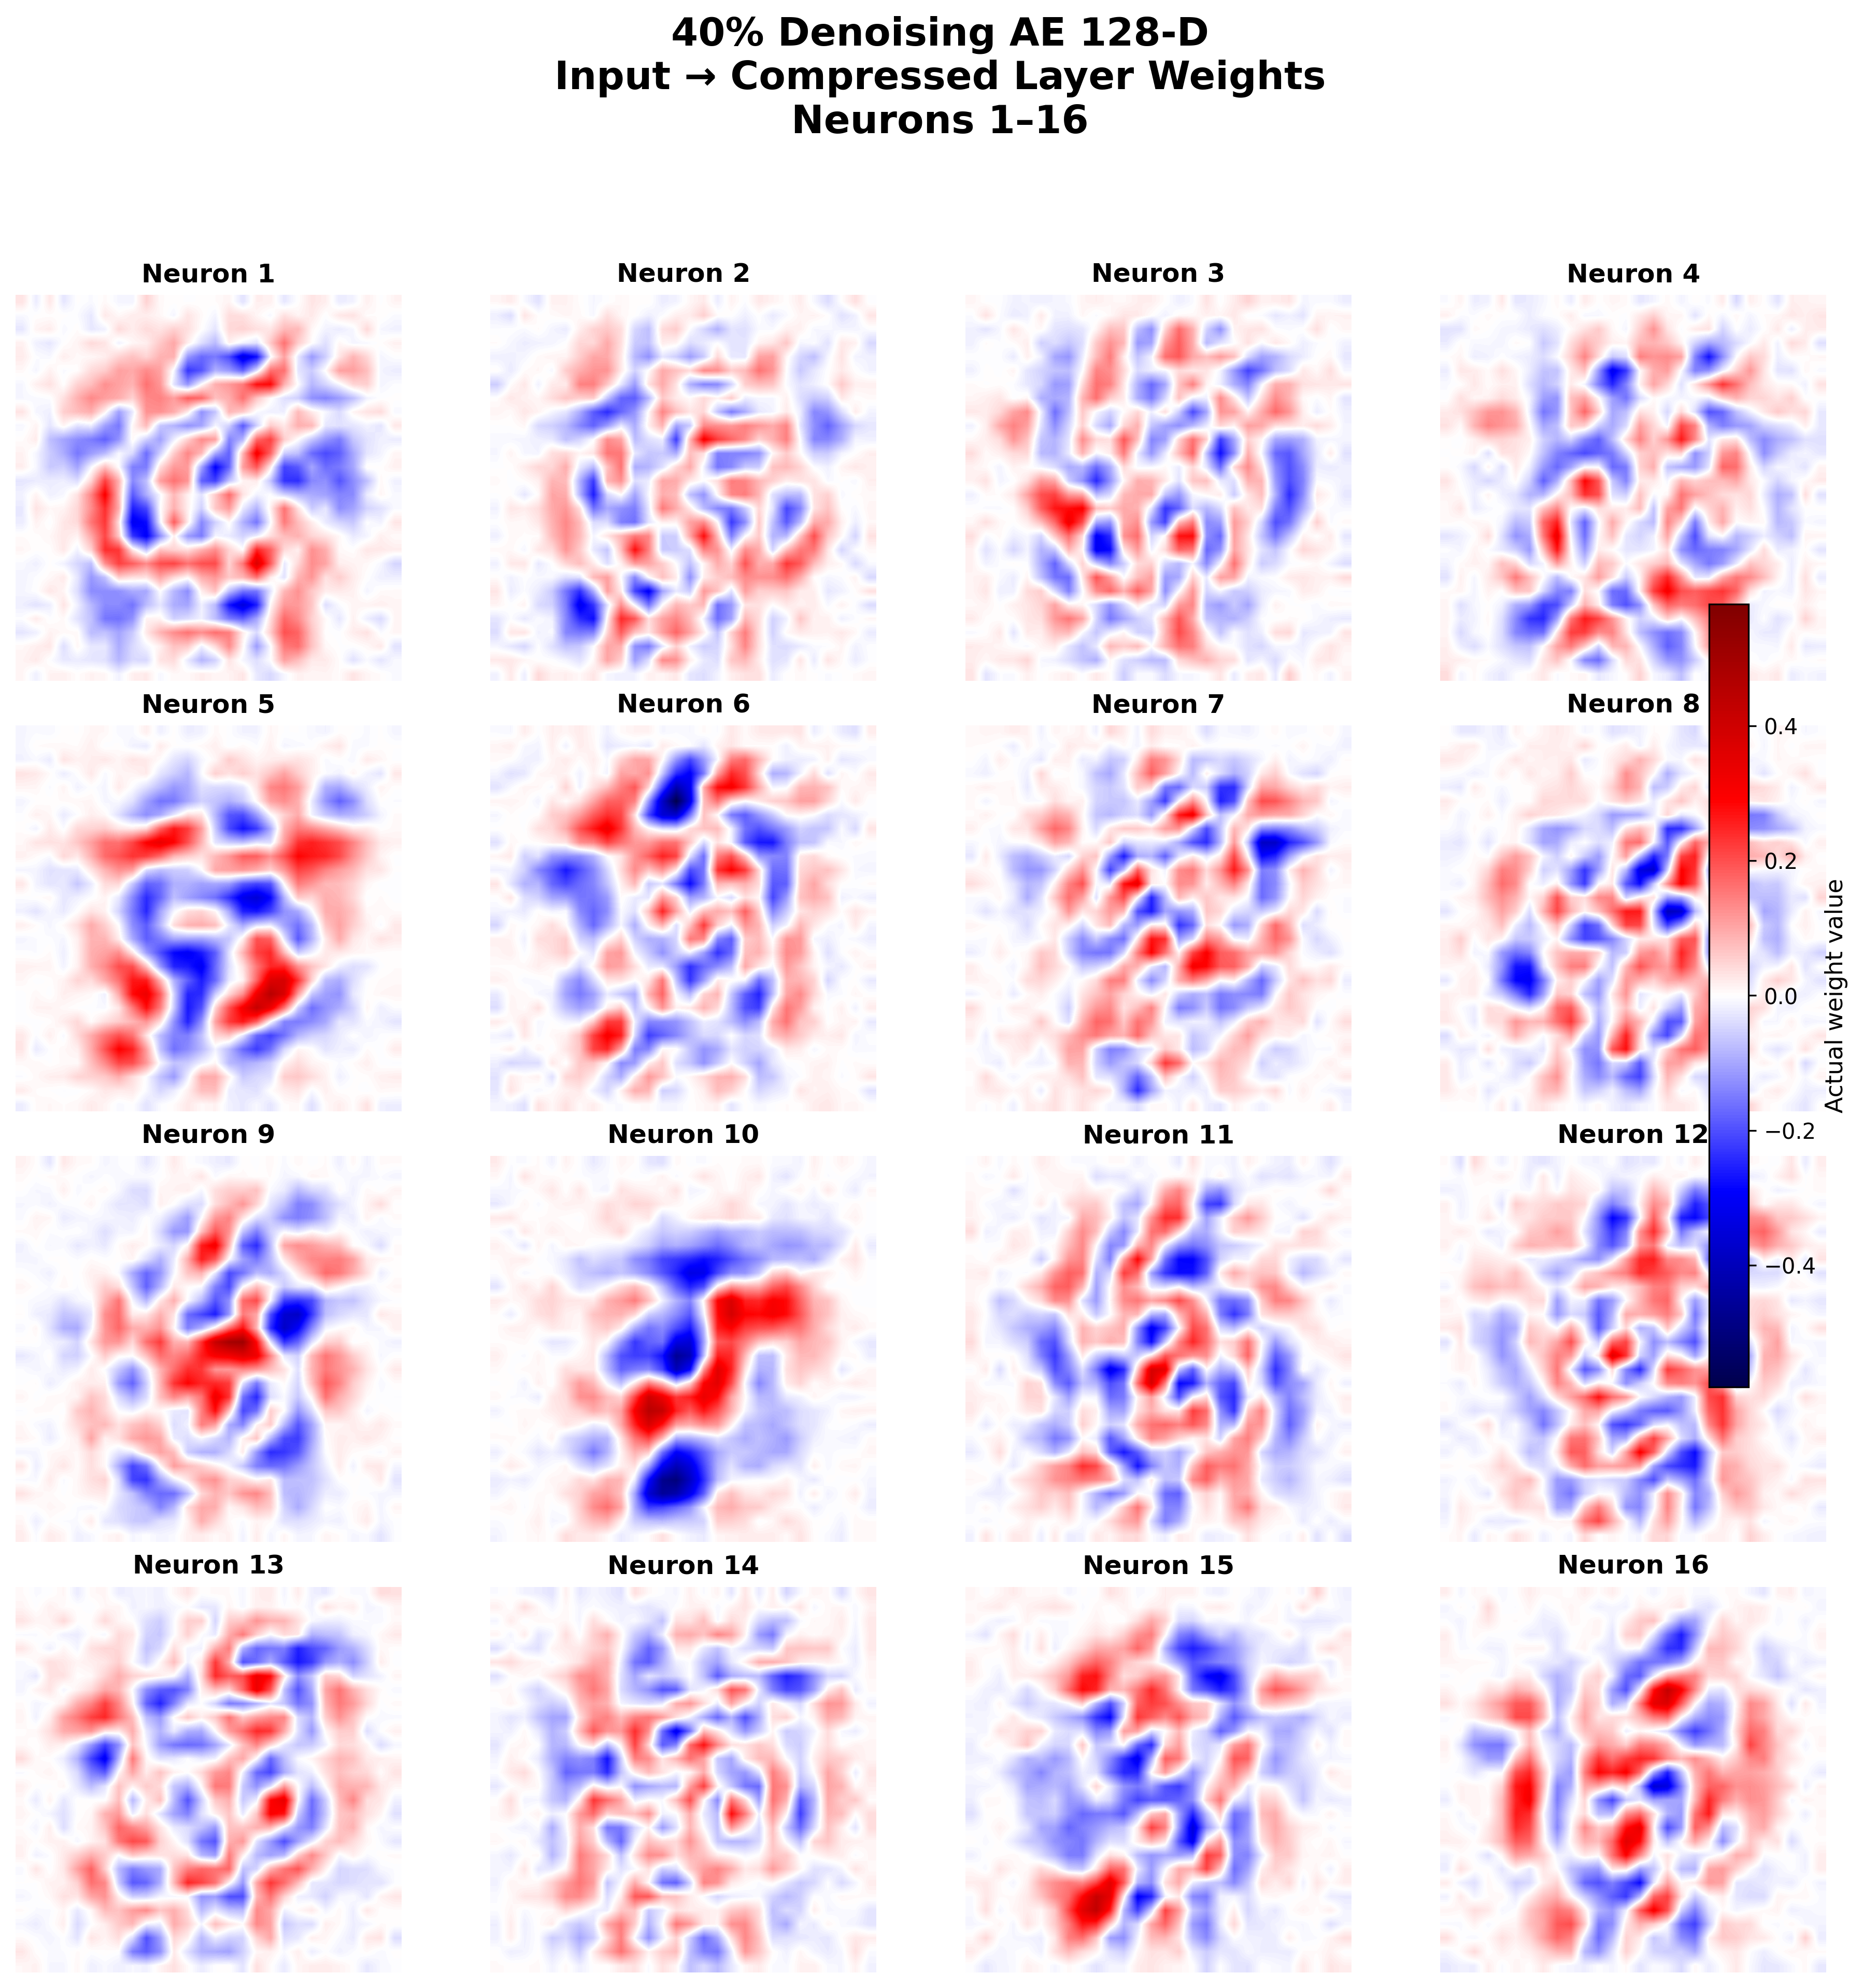
\includegraphics[width=0.99\linewidth,height=0.72\textheight,keepaspectratio]{figures/task6/40_pct_dae/neurons_001_016.png}
\caption{Input-to-bottleneck weight visualization for neurons 1--16.}
\label{fig:task6_17}
\end{figure}

\begin{figure}[H]
\centering
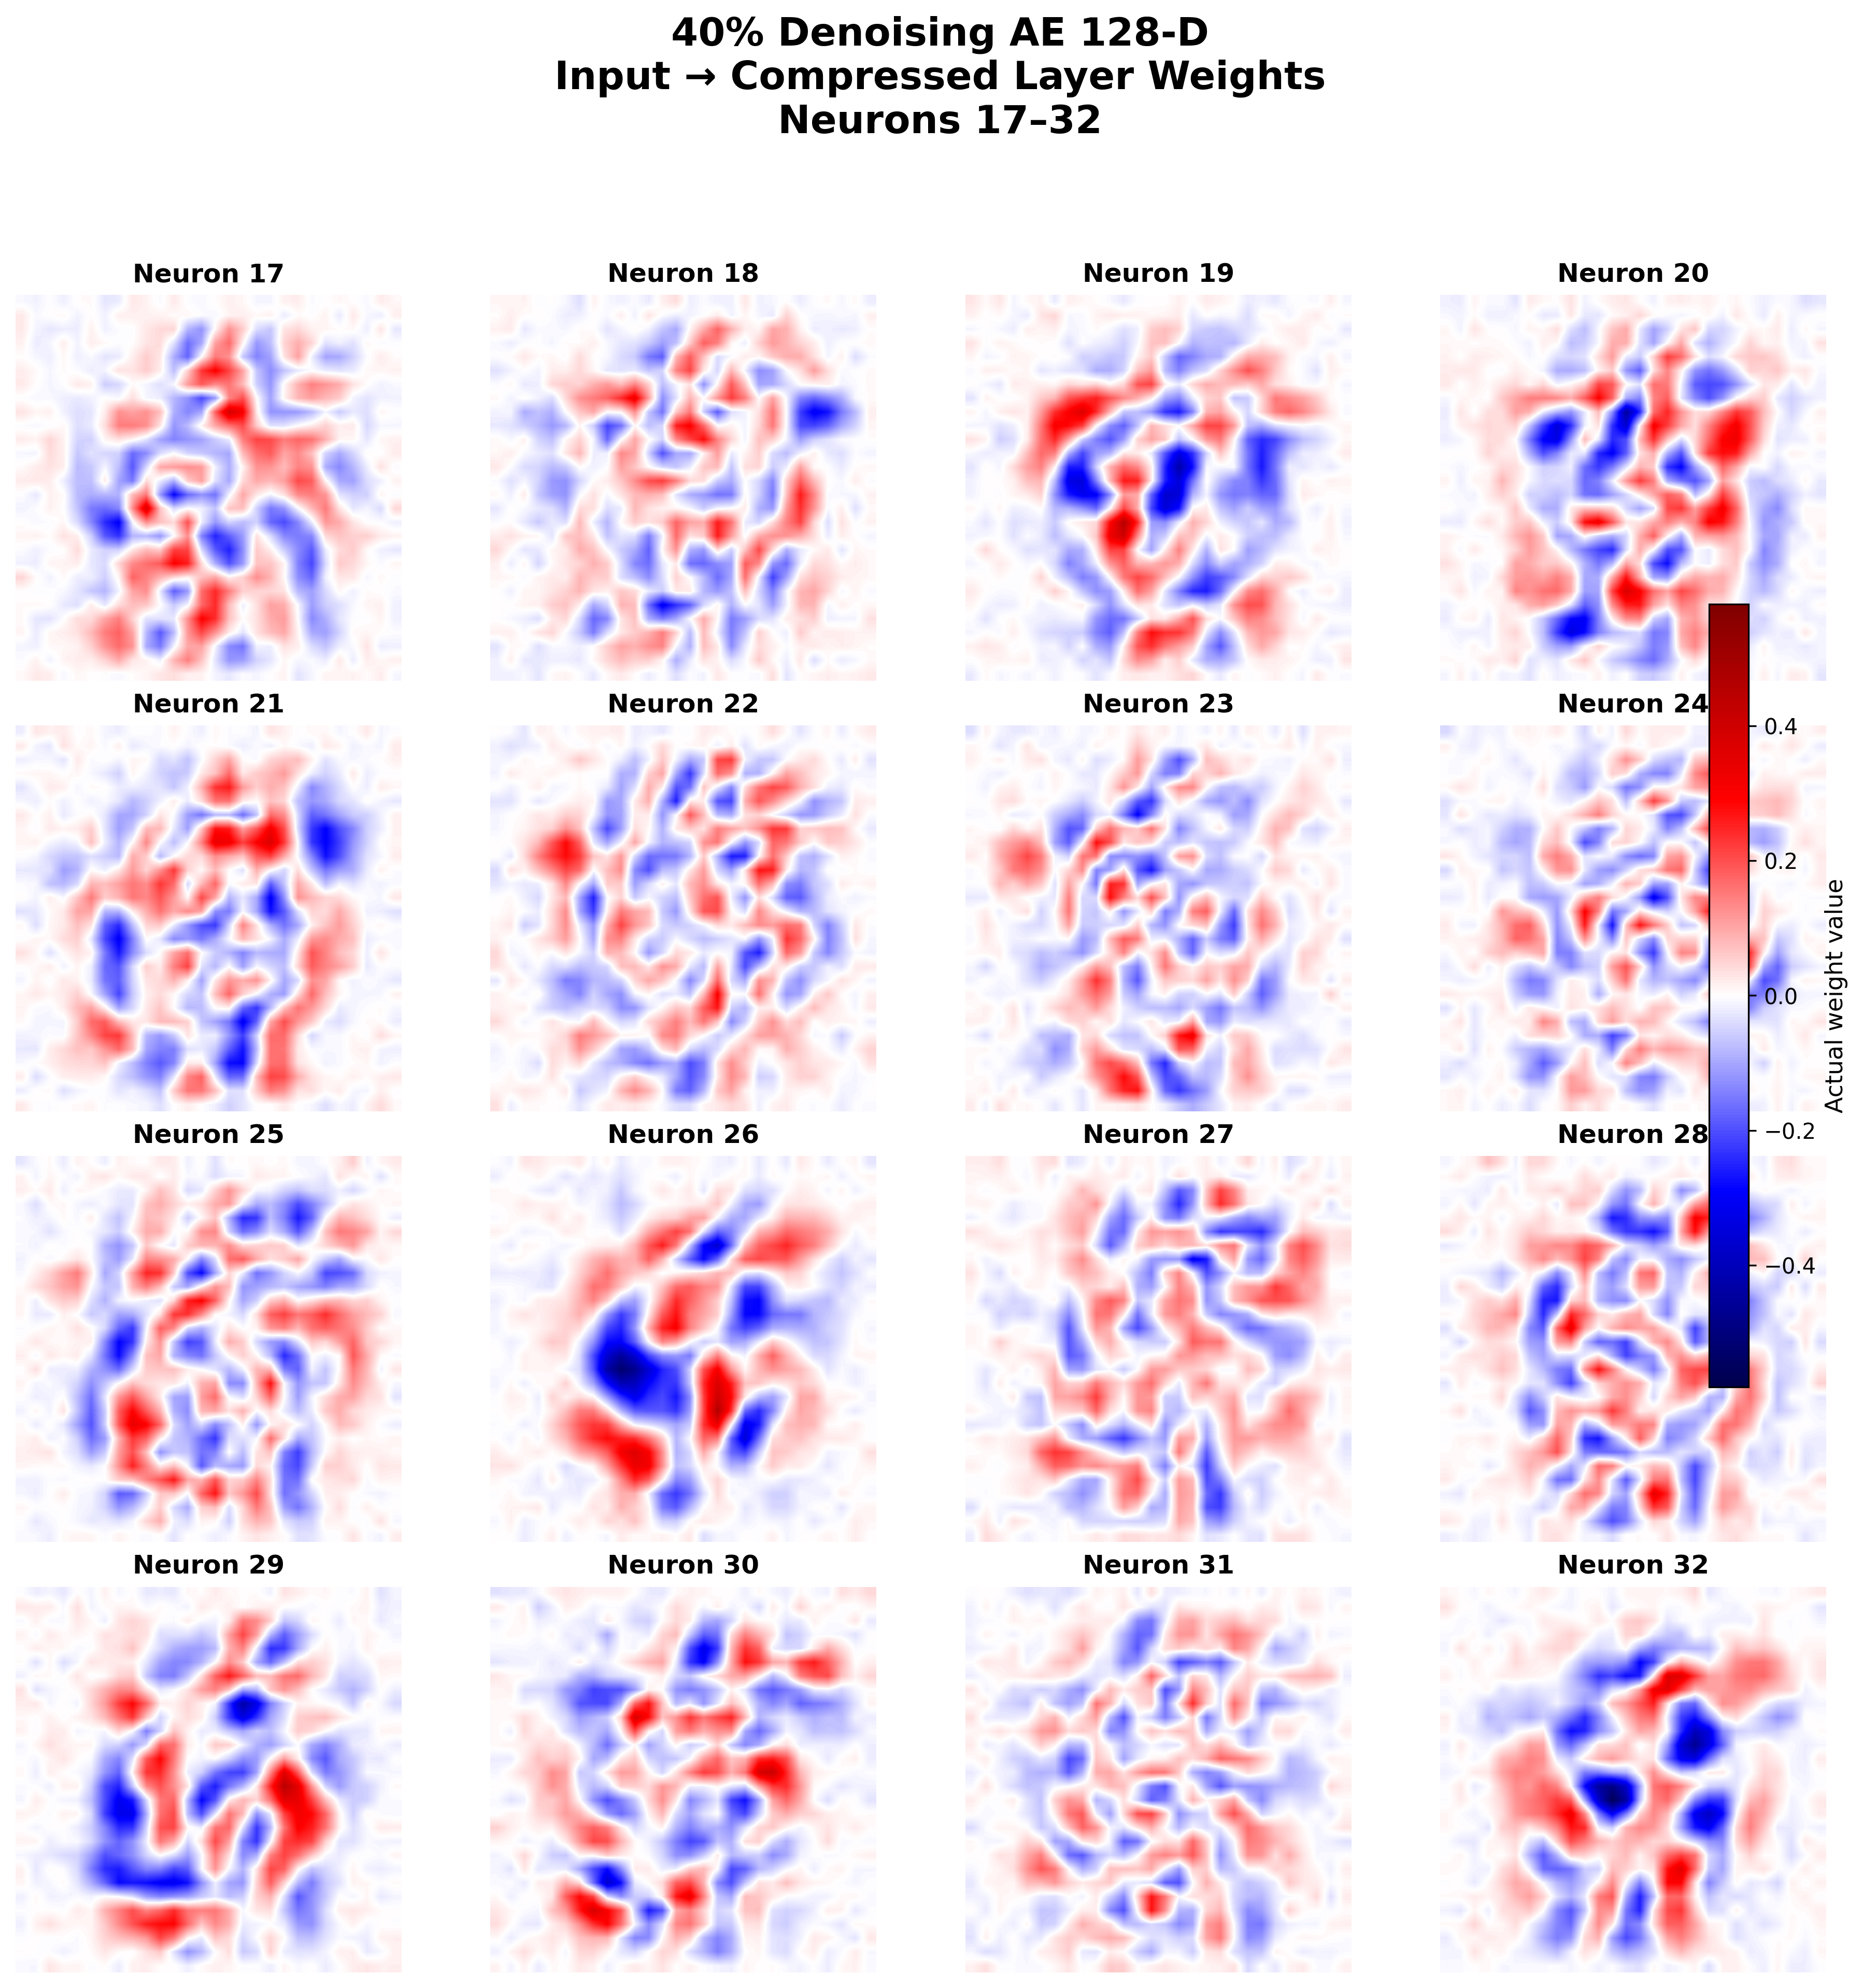
\includegraphics[width=0.99\linewidth,height=0.72\textheight,keepaspectratio]{figures/task6/40_pct_dae/neurons_017_032.png}
\caption{Input-to-bottleneck weight visualization for neurons 17--32.}
\label{fig:task6_18}
\end{figure}

\begin{figure}[H]
\centering
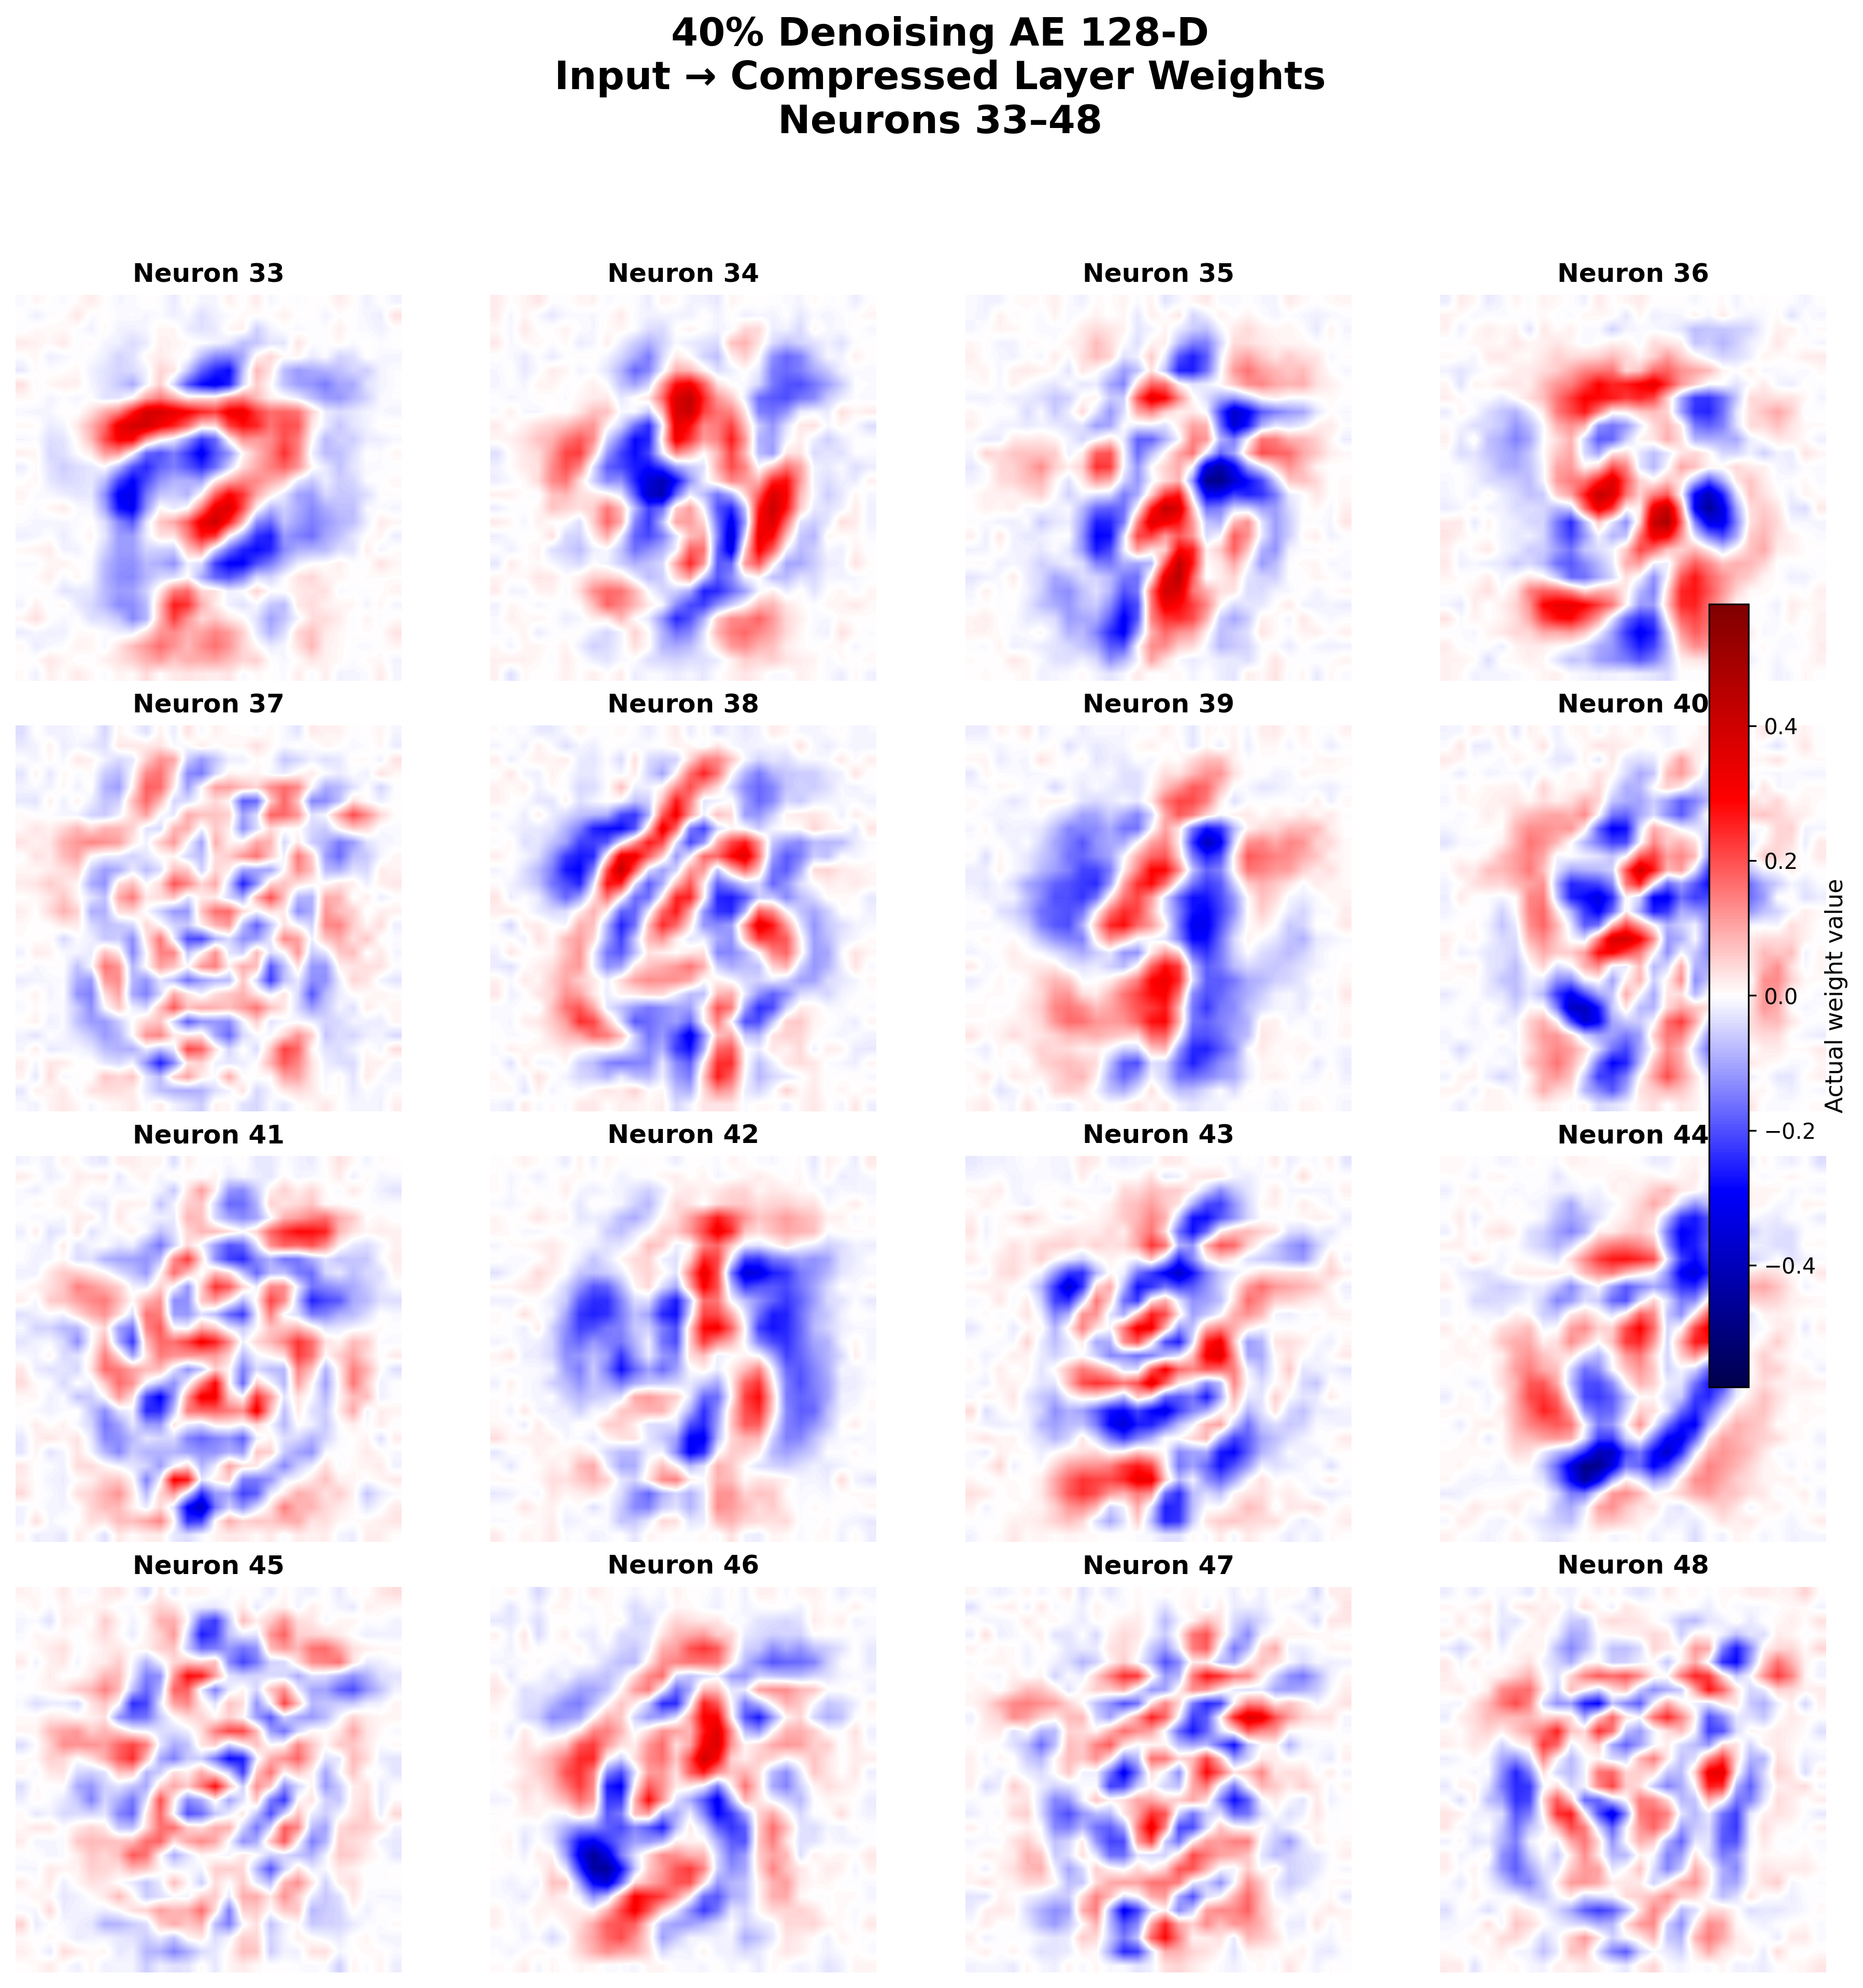
\includegraphics[width=0.99\linewidth,height=0.72\textheight,keepaspectratio]{figures/task6/40_pct_dae/neurons_033_048.png}
\caption{Input-to-bottleneck weight visualization for neurons 33--48.}
\label{fig:task6_19}
\end{figure}

\begin{figure}[H]
\centering
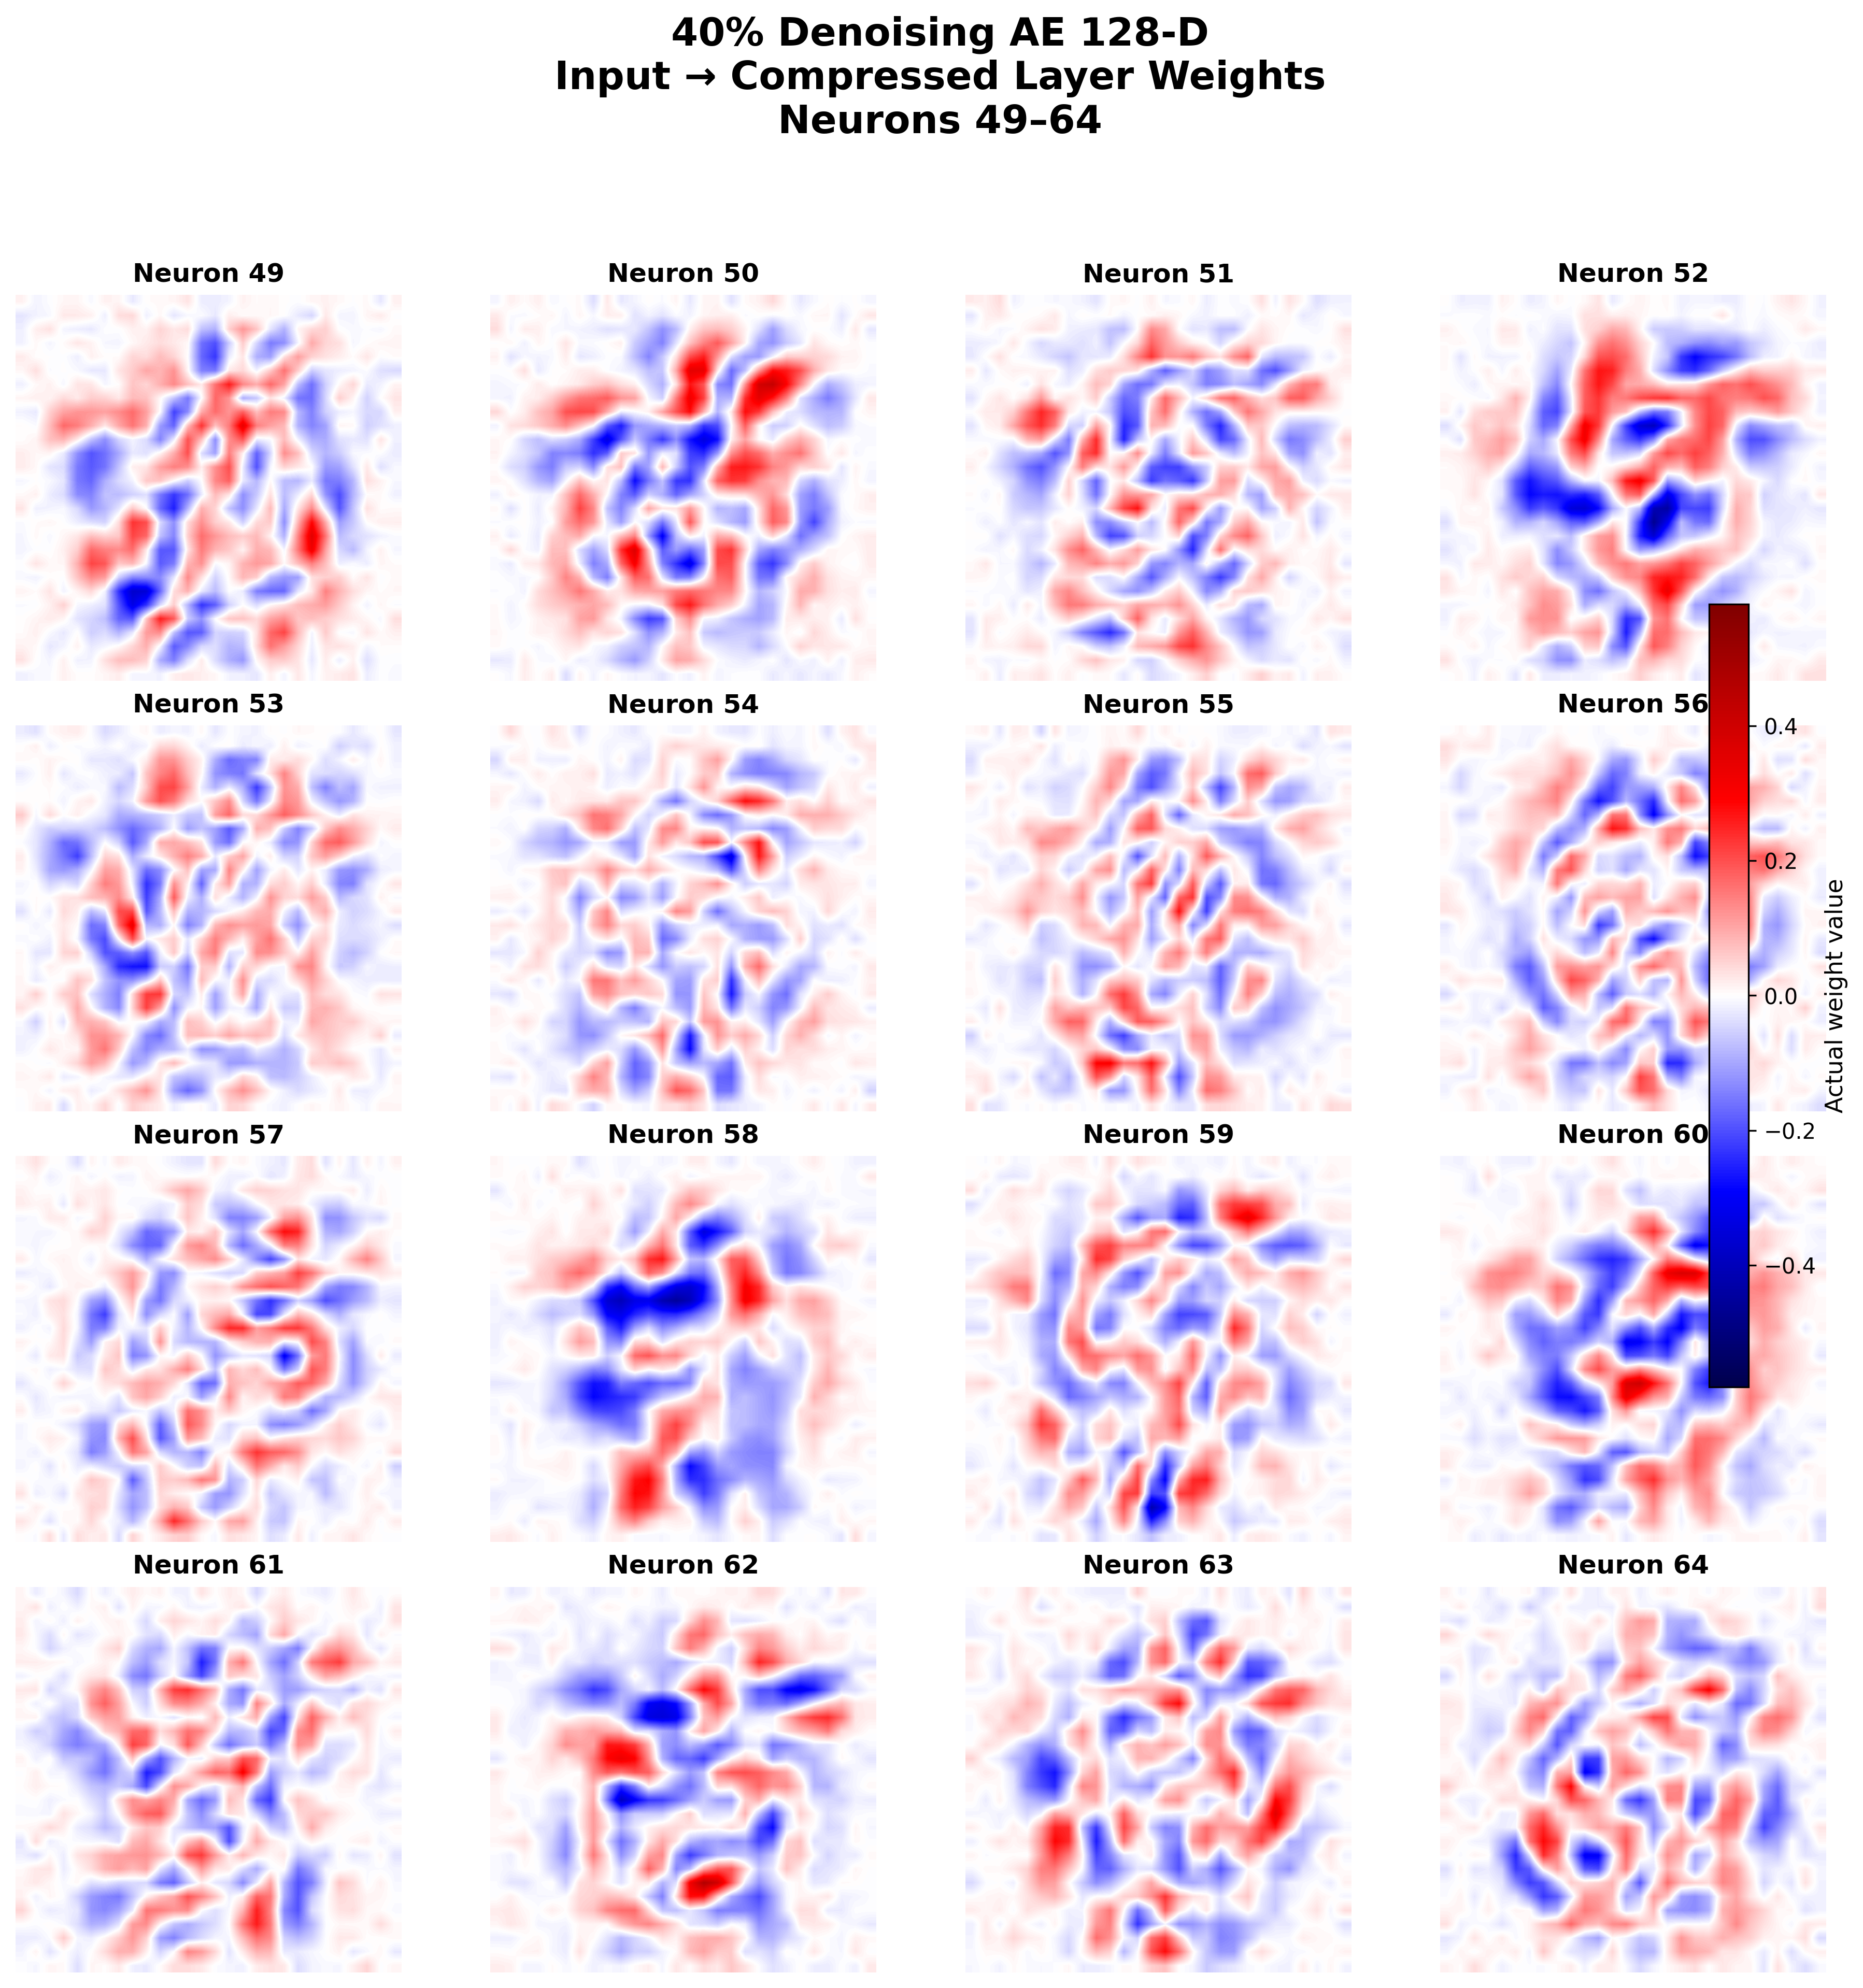
\includegraphics[width=0.99\linewidth,height=0.72\textheight,keepaspectratio]{figures/task6/40_pct_dae/neurons_049_064.png}
\caption{Input-to-bottleneck weight visualization for neurons 49--64.}
\label{fig:task6_20}
\end{figure}

\begin{figure}[H]
\centering
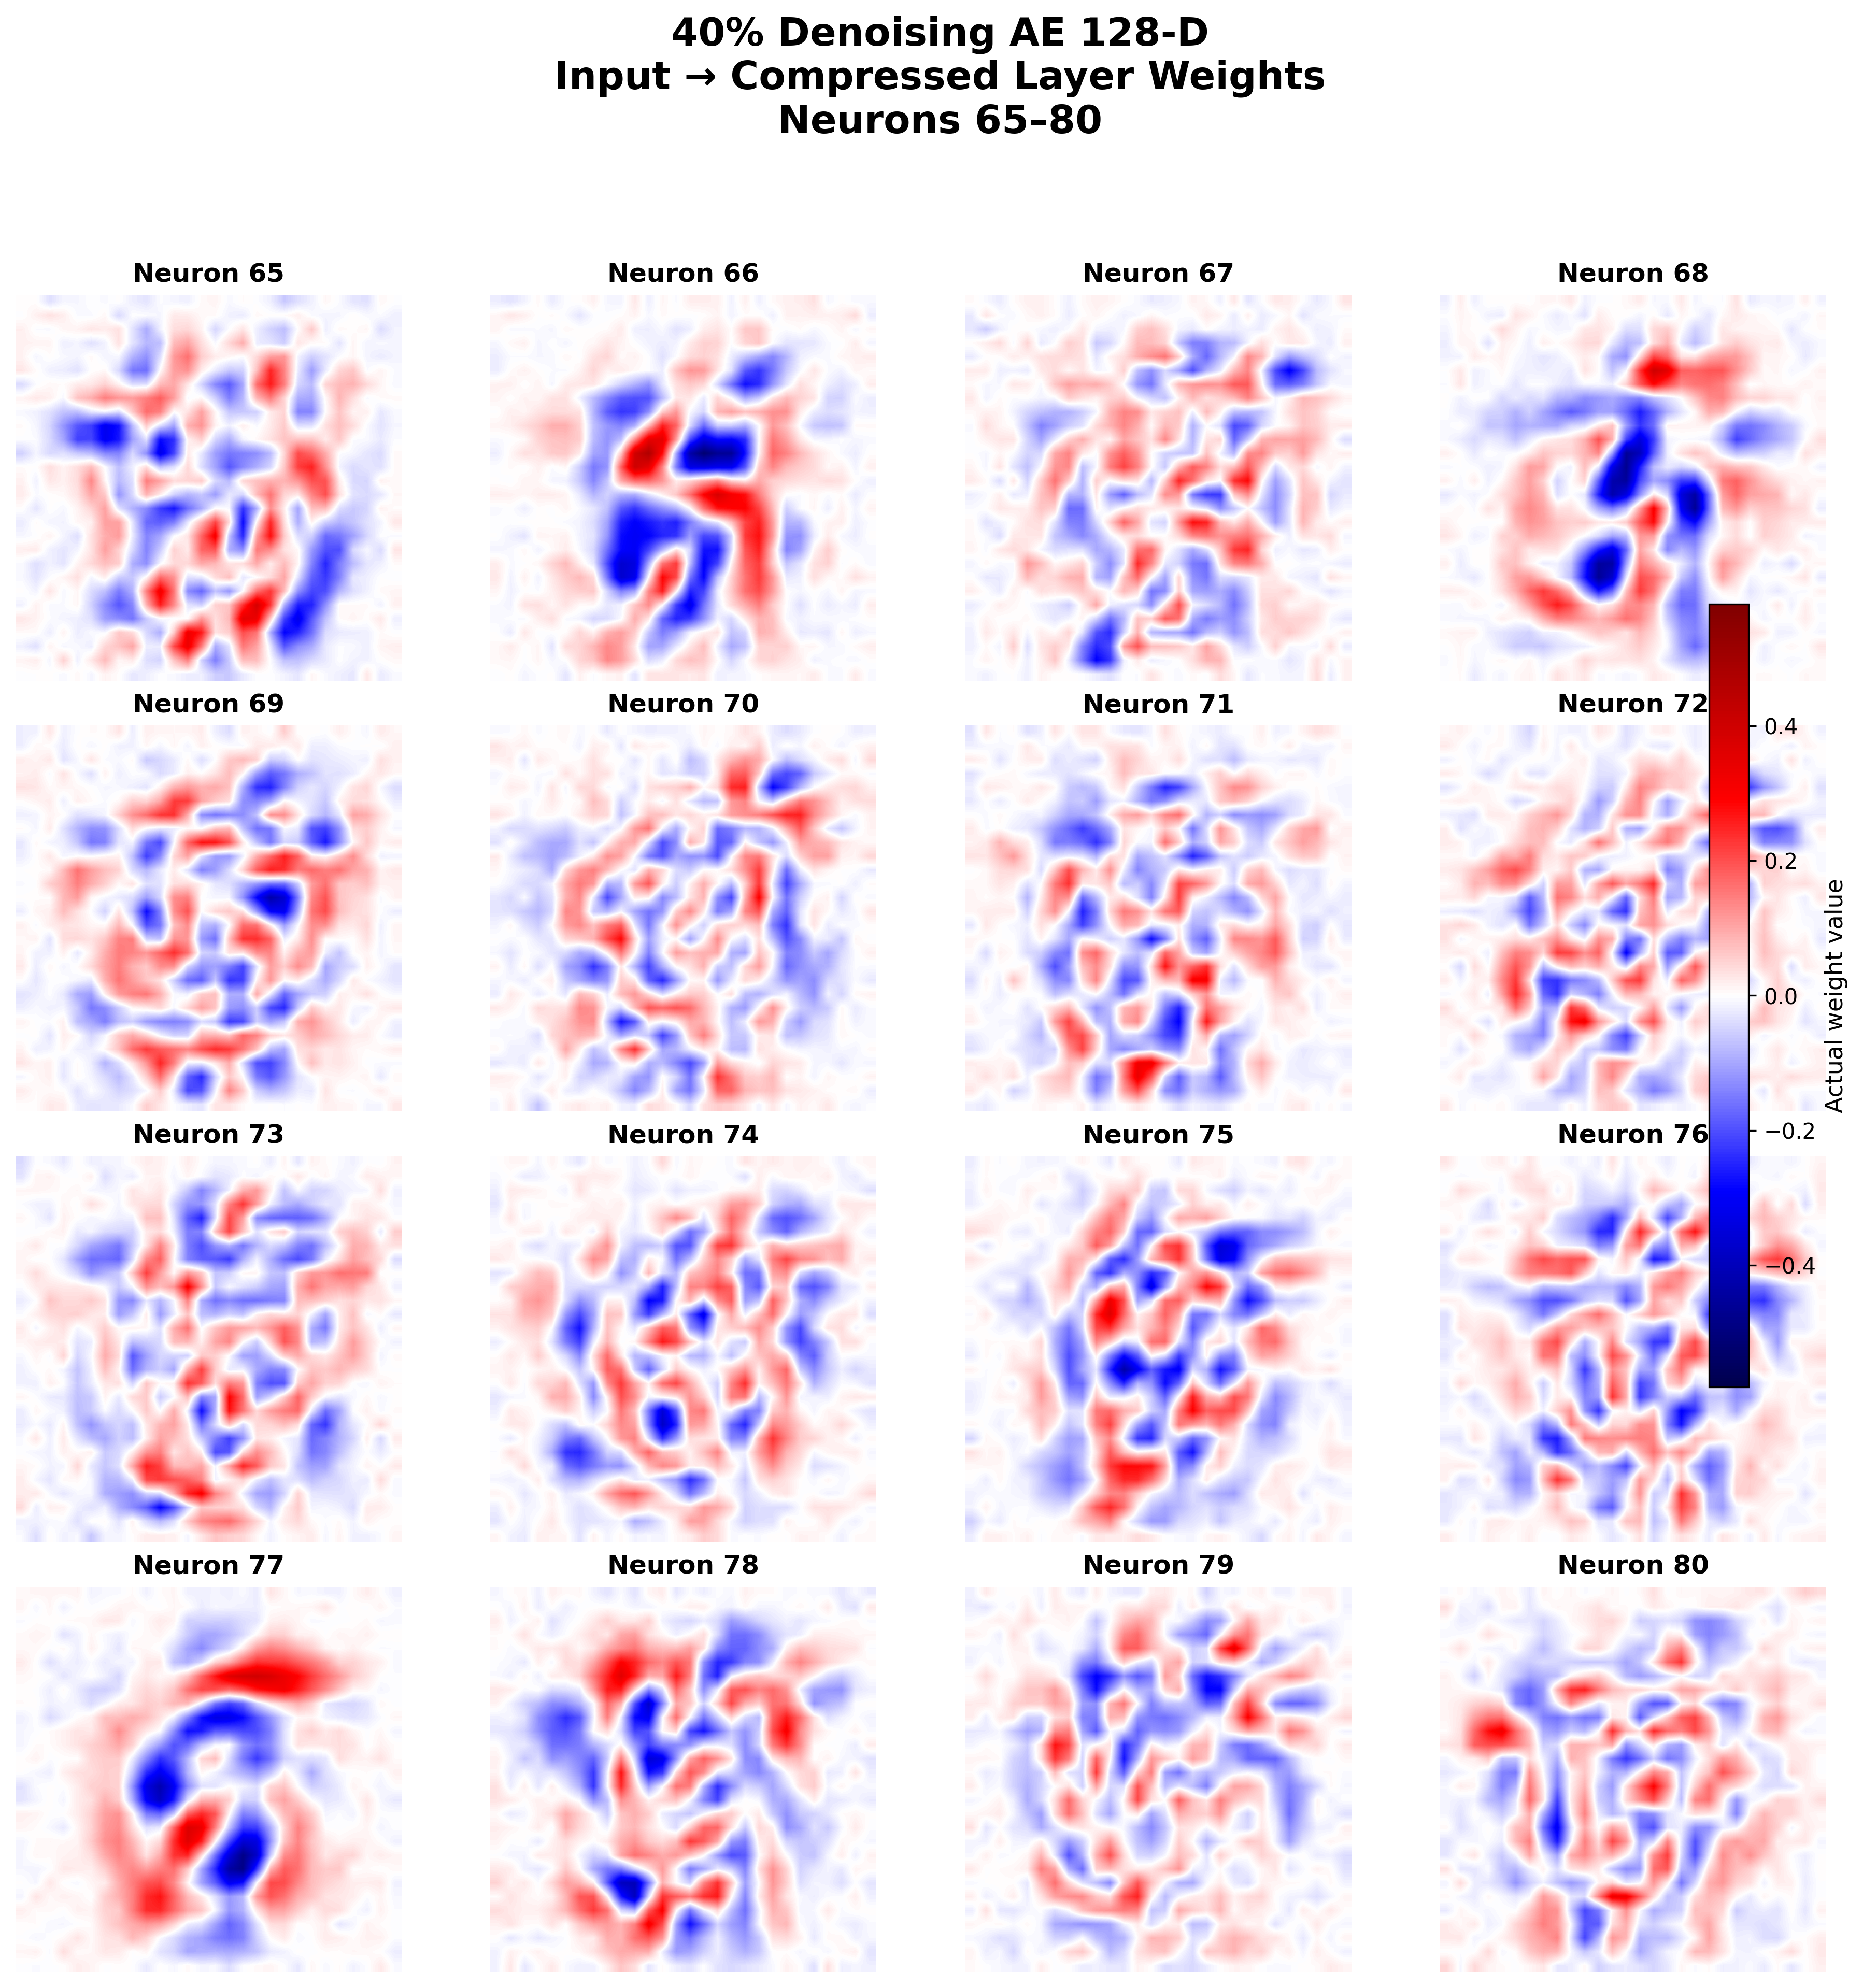
\includegraphics[width=0.99\linewidth,height=0.72\textheight,keepaspectratio]{figures/task6/40_pct_dae/neurons_065_080.png}
\caption{Input-to-bottleneck weight visualization for neurons 65--80.}
\label{fig:task6_21}
\end{figure}

\begin{figure}[H]
\centering
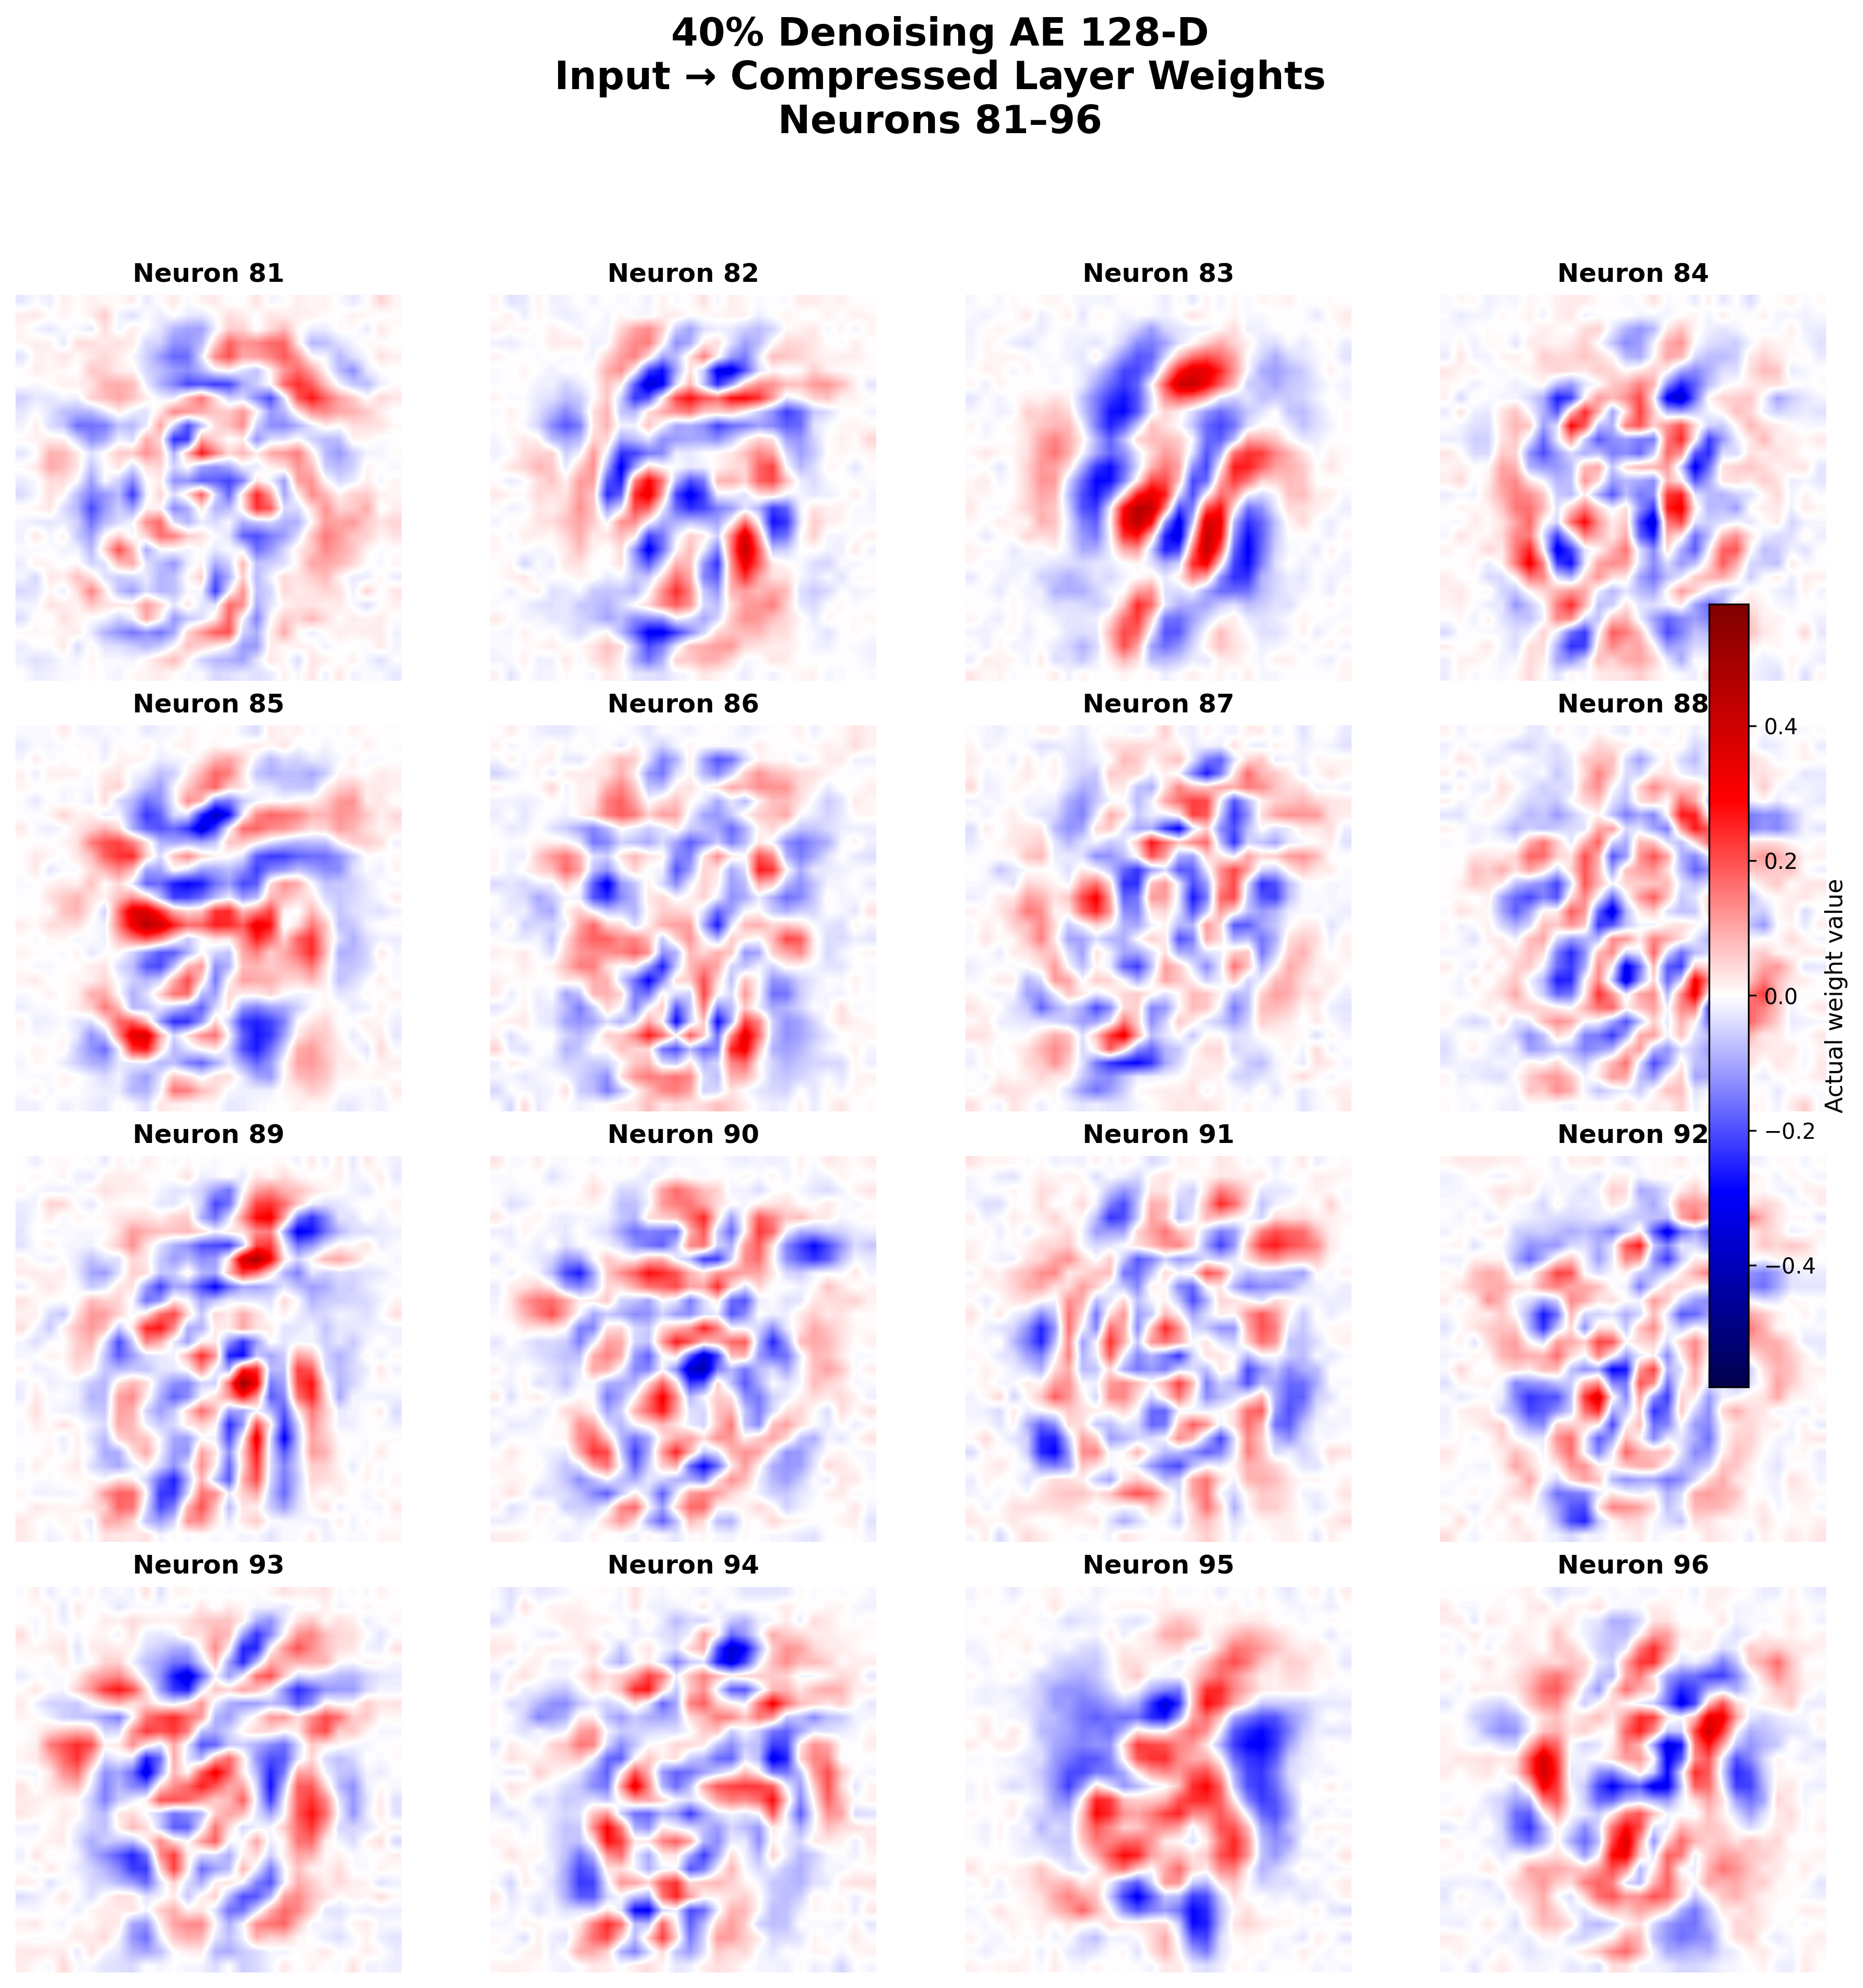
\includegraphics[width=0.99\linewidth,height=0.72\textheight,keepaspectratio]{figures/task6/40_pct_dae/neurons_081_096.png}
\caption{Input-to-bottleneck weight visualization for neurons 81--96.}
\label{fig:task6_22}
\end{figure}

\begin{figure}[H]
\centering
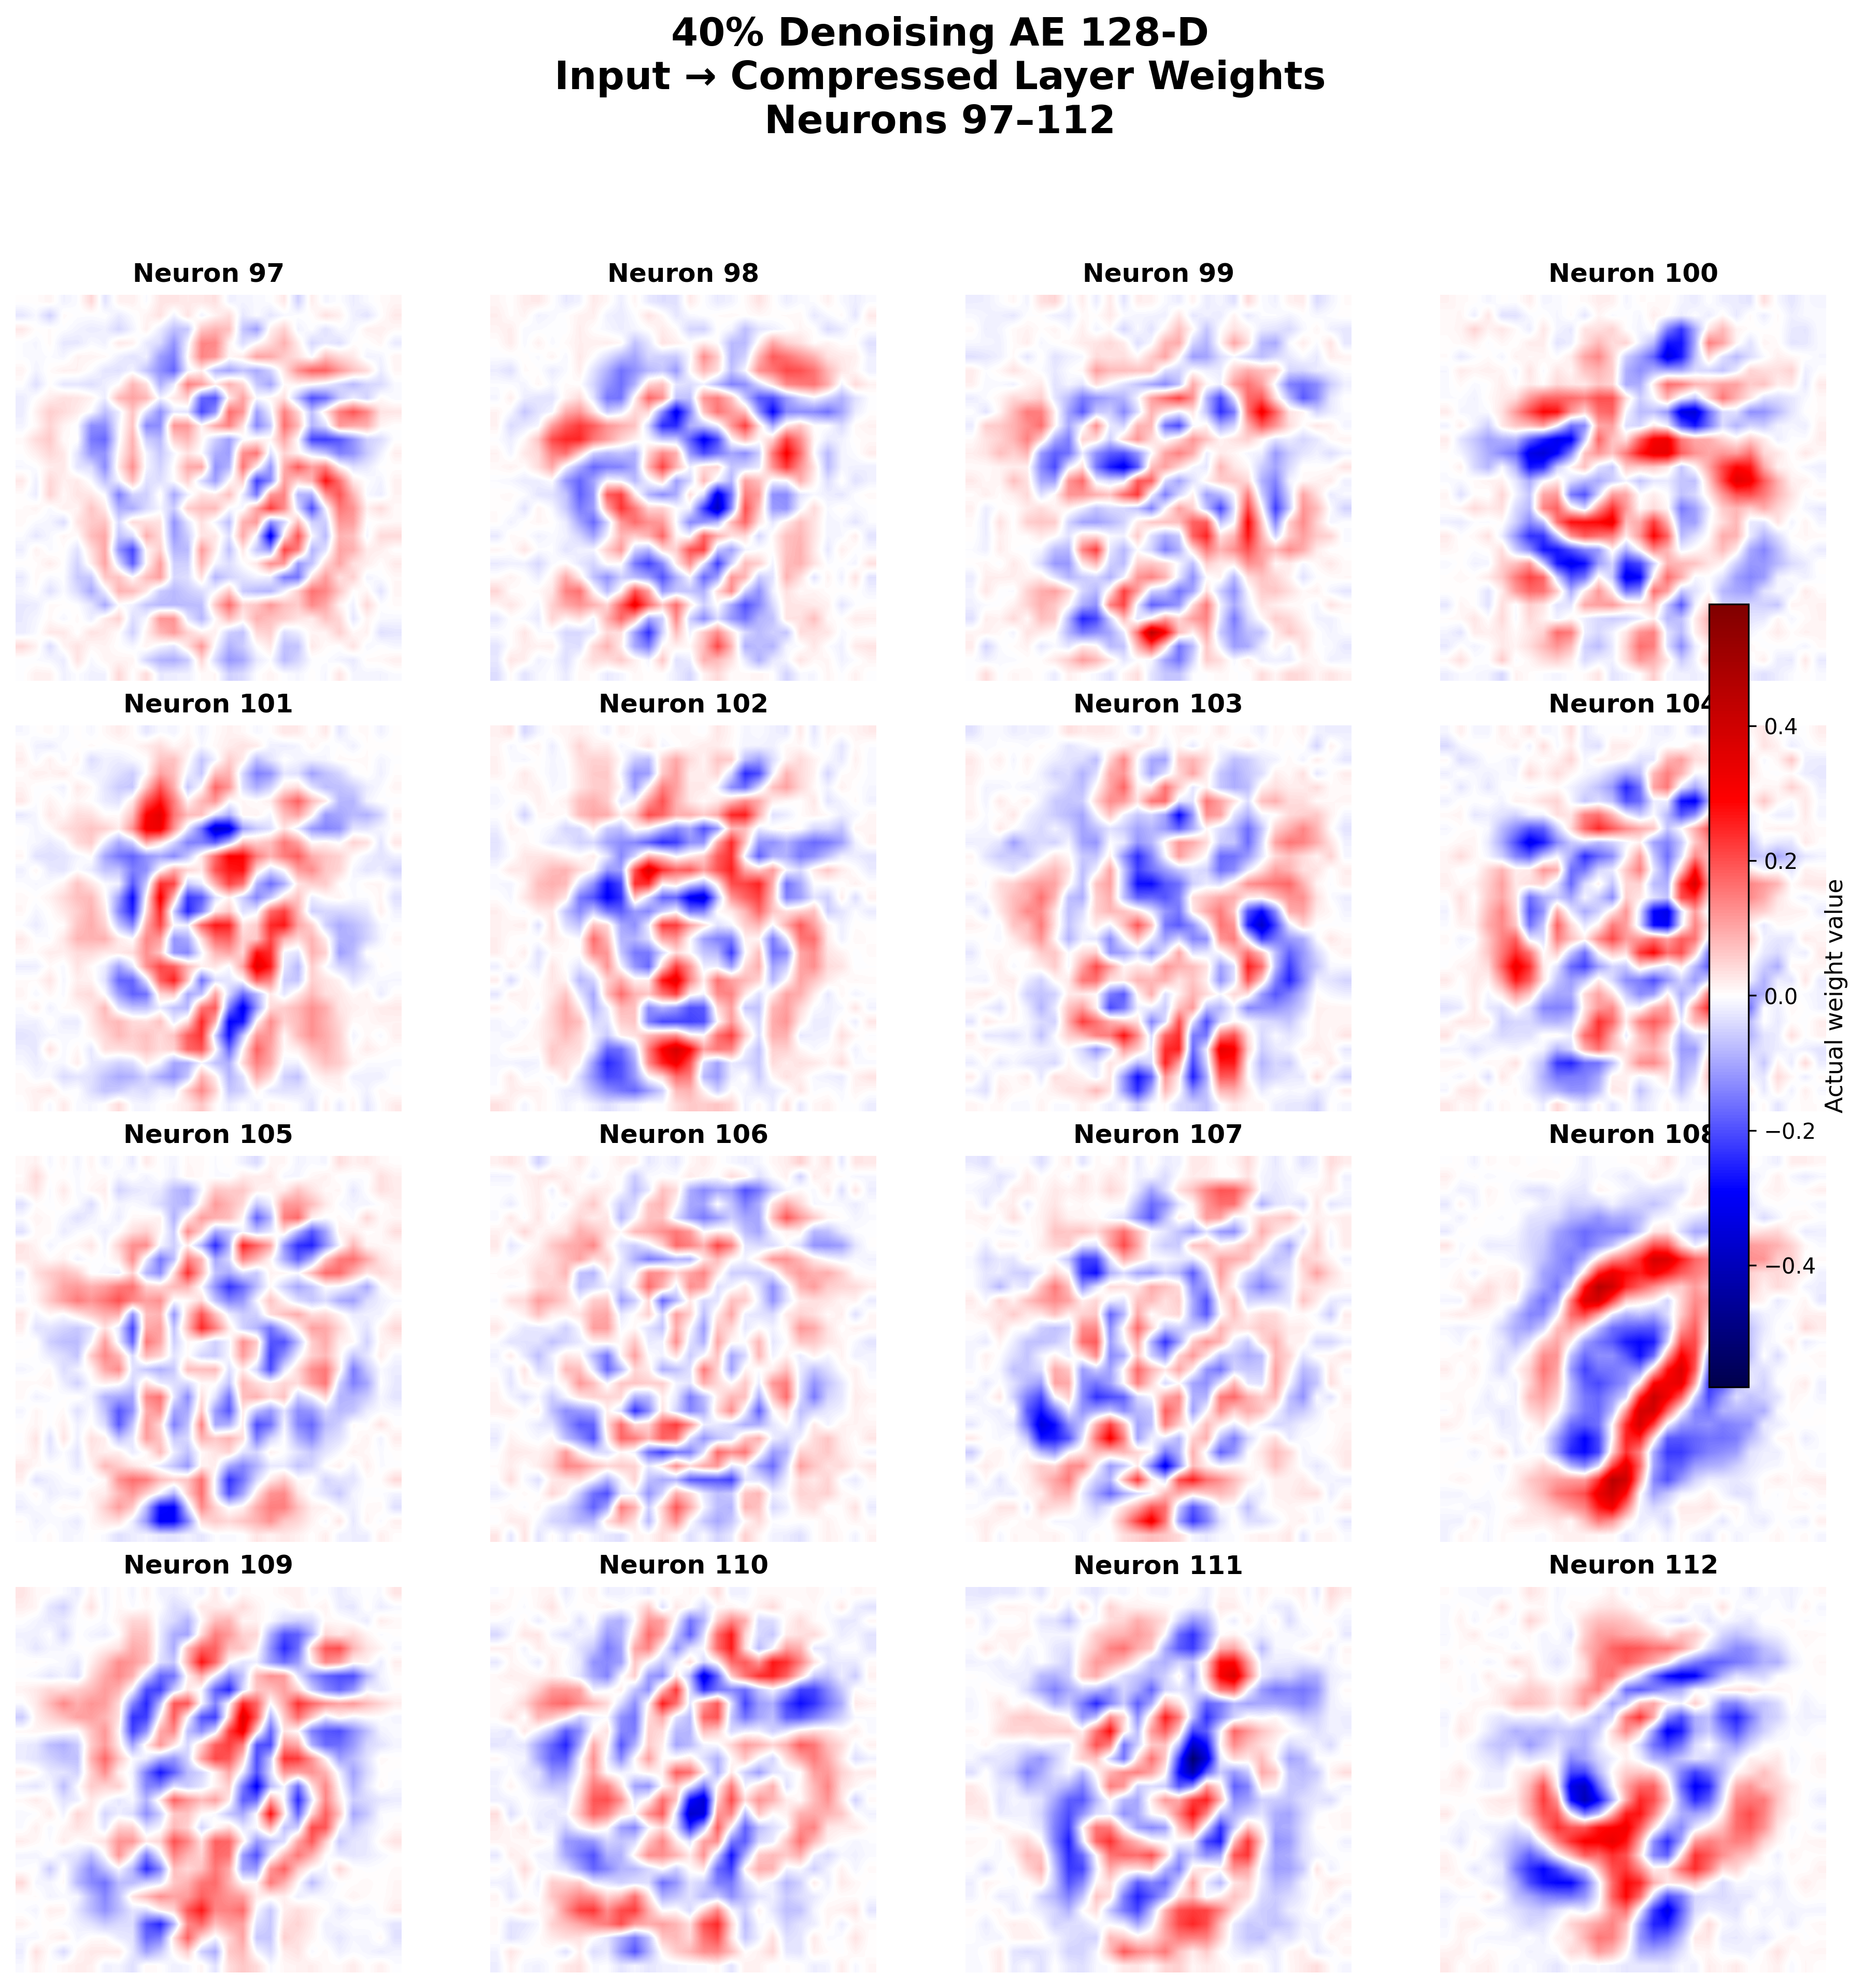
\includegraphics[width=0.99\linewidth,height=0.72\textheight,keepaspectratio]{figures/task6/40_pct_dae/neurons_097_112.png}
\caption{Input-to-bottleneck weight visualization for neurons 97--112.}
\label{fig:task6_23}
\end{figure}

\begin{figure}[H]
\centering
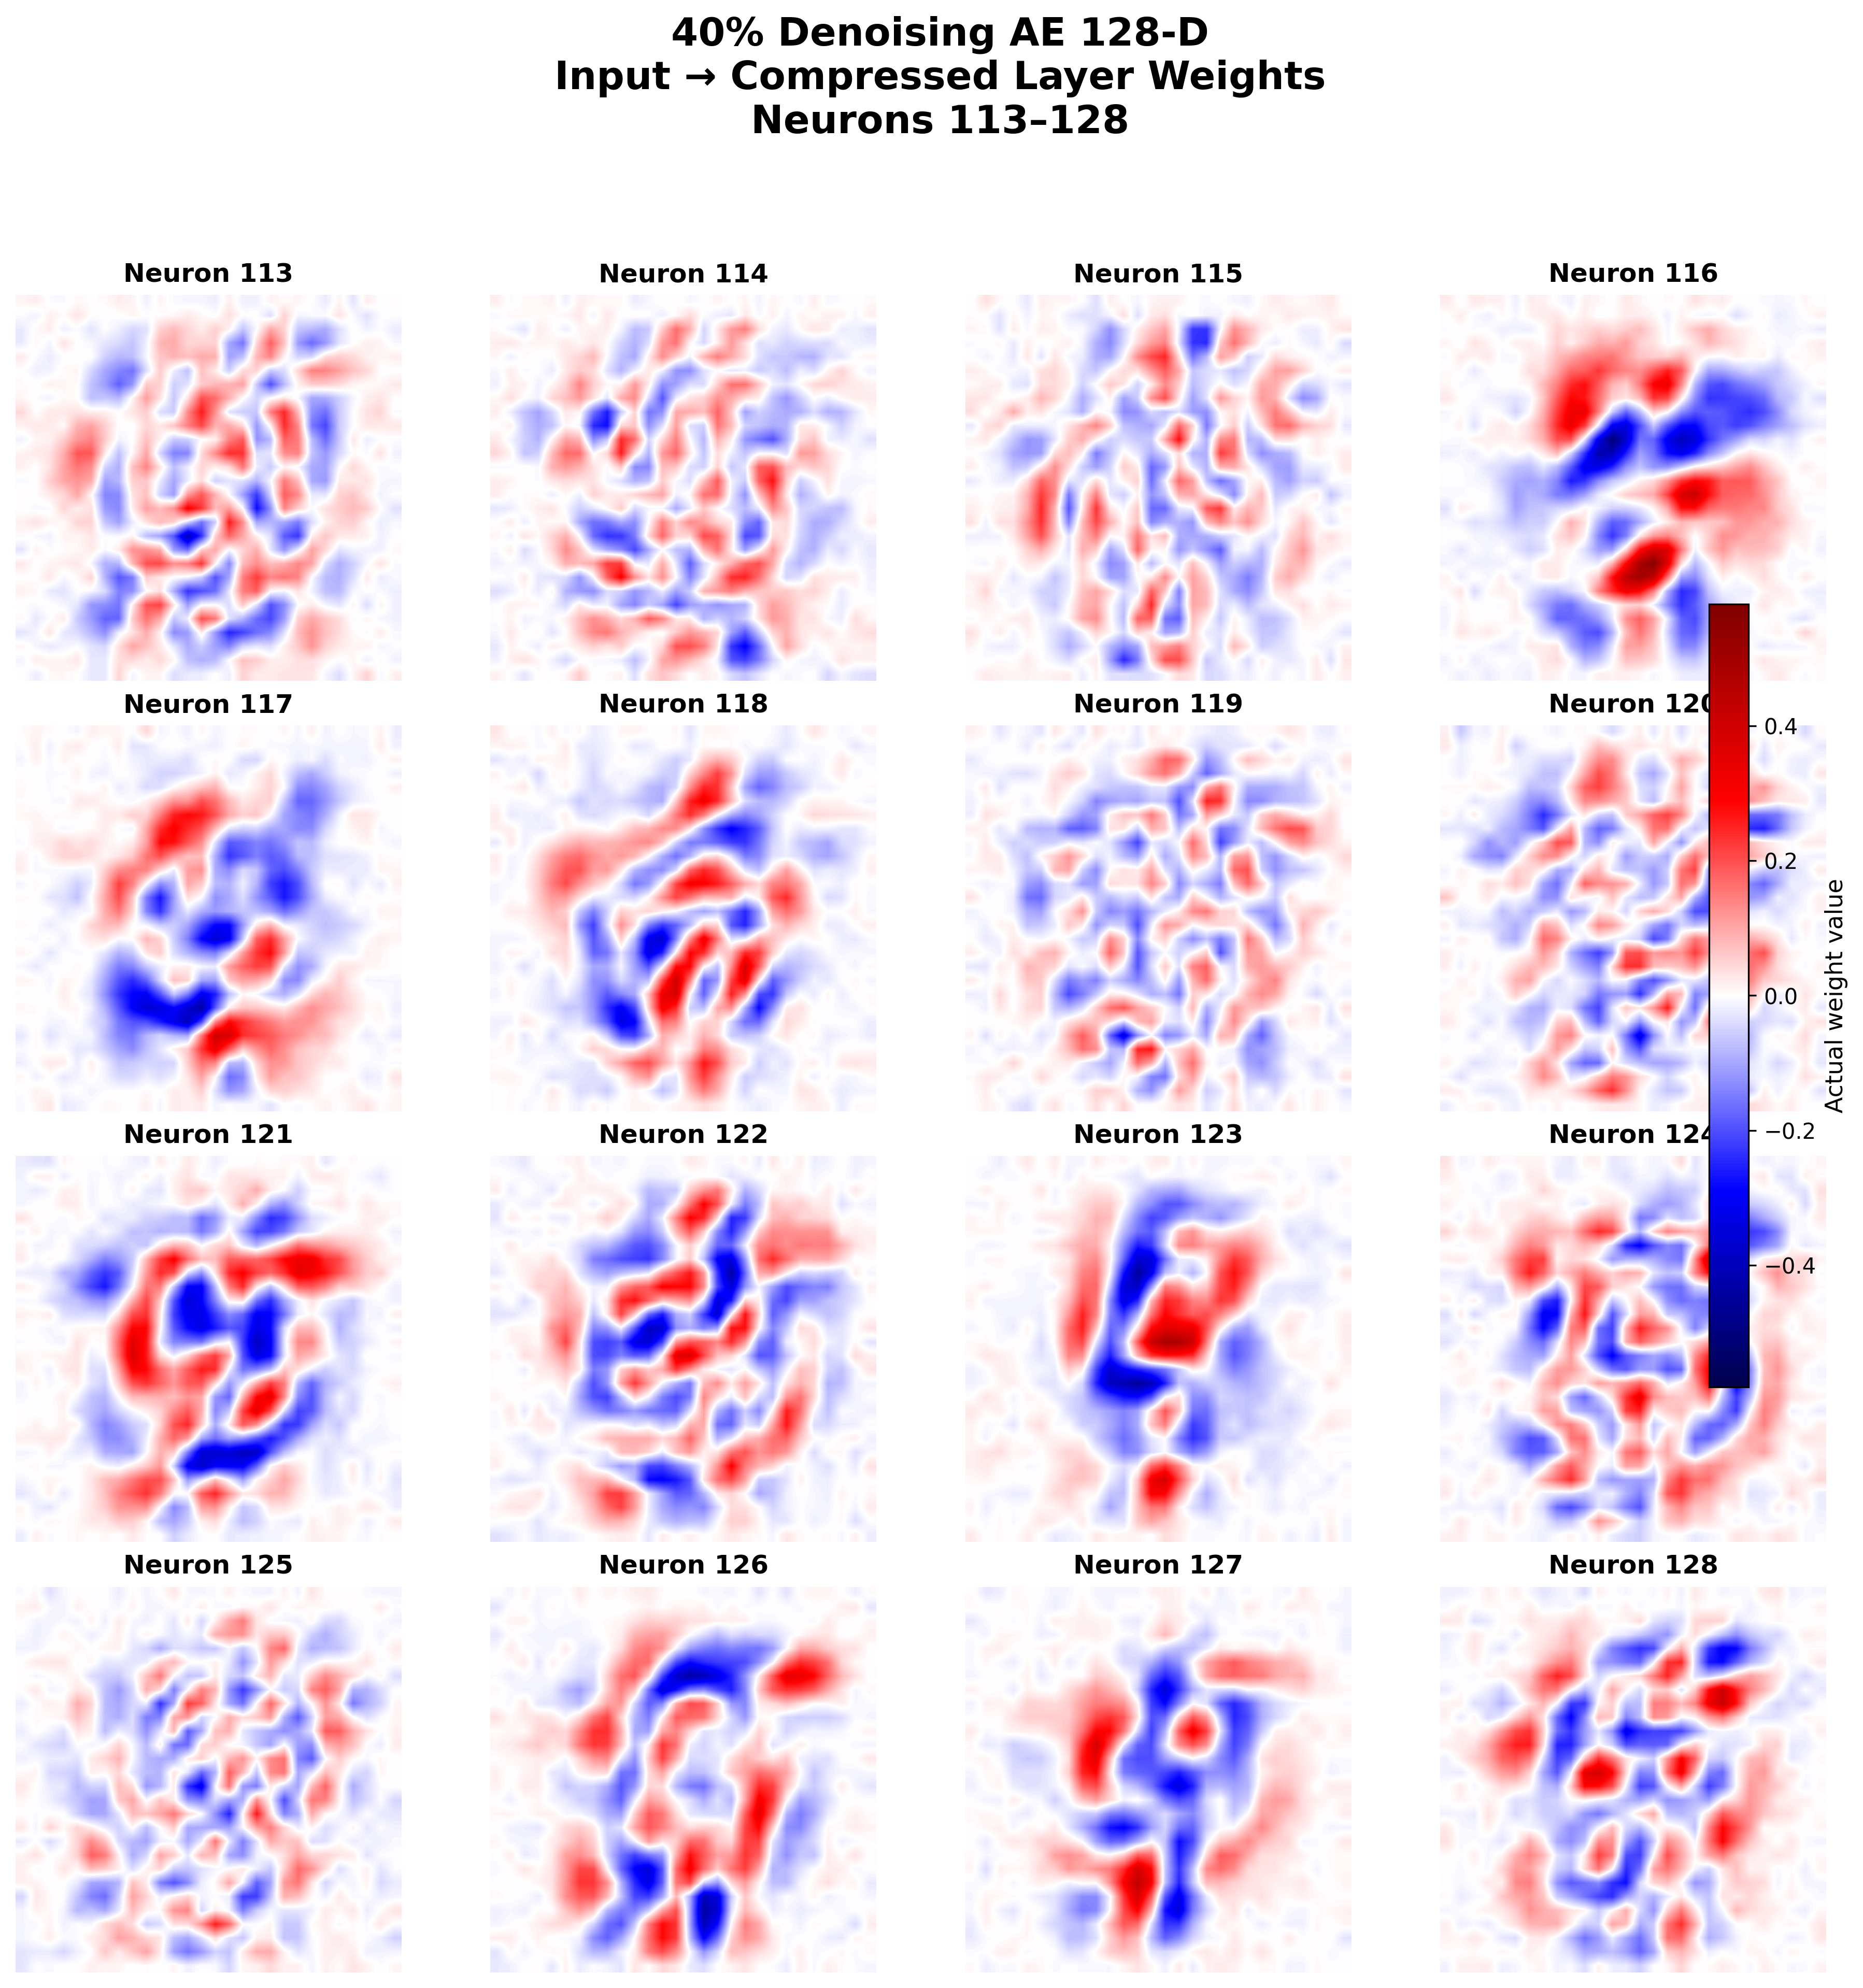
\includegraphics[width=0.99\linewidth,height=0.72\textheight,keepaspectratio]{figures/task6/40_pct_dae/neurons_113_128.png}
\caption{Input-to-bottleneck weight visualization for neurons 113--128.}
\label{fig:task6_24}
\end{figure}
